% Options for packages loaded elsewhere
\PassOptionsToPackage{unicode}{hyperref}
\PassOptionsToPackage{hyphens}{url}
%
\documentclass[
]{book}
\usepackage{amsmath,amssymb}
\usepackage{iftex}
\ifPDFTeX
  \usepackage[T1]{fontenc}
  \usepackage[utf8]{inputenc}
  \usepackage{textcomp} % provide euro and other symbols
\else % if luatex or xetex
  \usepackage{unicode-math} % this also loads fontspec
  \defaultfontfeatures{Scale=MatchLowercase}
  \defaultfontfeatures[\rmfamily]{Ligatures=TeX,Scale=1}
\fi
\usepackage{lmodern}
\ifPDFTeX\else
  % xetex/luatex font selection
\fi
% Use upquote if available, for straight quotes in verbatim environments
\IfFileExists{upquote.sty}{\usepackage{upquote}}{}
\IfFileExists{microtype.sty}{% use microtype if available
  \usepackage[]{microtype}
  \UseMicrotypeSet[protrusion]{basicmath} % disable protrusion for tt fonts
}{}
\makeatletter
\@ifundefined{KOMAClassName}{% if non-KOMA class
  \IfFileExists{parskip.sty}{%
    \usepackage{parskip}
  }{% else
    \setlength{\parindent}{0pt}
    \setlength{\parskip}{6pt plus 2pt minus 1pt}}
}{% if KOMA class
  \KOMAoptions{parskip=half}}
\makeatother
\usepackage{xcolor}
\usepackage{longtable,booktabs,array}
\usepackage{calc} % for calculating minipage widths
% Correct order of tables after \paragraph or \subparagraph
\usepackage{etoolbox}
\makeatletter
\patchcmd\longtable{\par}{\if@noskipsec\mbox{}\fi\par}{}{}
\makeatother
% Allow footnotes in longtable head/foot
\IfFileExists{footnotehyper.sty}{\usepackage{footnotehyper}}{\usepackage{footnote}}
\makesavenoteenv{longtable}
\usepackage{graphicx}
\makeatletter
\def\maxwidth{\ifdim\Gin@nat@width>\linewidth\linewidth\else\Gin@nat@width\fi}
\def\maxheight{\ifdim\Gin@nat@height>\textheight\textheight\else\Gin@nat@height\fi}
\makeatother
% Scale images if necessary, so that they will not overflow the page
% margins by default, and it is still possible to overwrite the defaults
% using explicit options in \includegraphics[width, height, ...]{}
\setkeys{Gin}{width=\maxwidth,height=\maxheight,keepaspectratio}
% Set default figure placement to htbp
\makeatletter
\def\fps@figure{htbp}
\makeatother
\setlength{\emergencystretch}{3em} % prevent overfull lines
\providecommand{\tightlist}{%
  \setlength{\itemsep}{0pt}\setlength{\parskip}{0pt}}
\setcounter{secnumdepth}{5}
\usepackage{booktabs}
\ifLuaTeX
  \usepackage{selnolig}  % disable illegal ligatures
\fi
\usepackage[]{natbib}
\bibliographystyle{plainnat}
\IfFileExists{bookmark.sty}{\usepackage{bookmark}}{\usepackage{hyperref}}
\IfFileExists{xurl.sty}{\usepackage{xurl}}{} % add URL line breaks if available
\urlstyle{same}
\hypersetup{
  pdftitle={EEBE Estadística},
  pdfauthor={Alejandro Cáceres (alejandro.caceres.dominguez@upc.edu)},
  hidelinks,
  pdfcreator={LaTeX via pandoc}}

\title{EEBE Estadística}
\author{Alejandro Cáceres (\href{mailto:alejandro.caceres.dominguez@upc.edu}{\nolinkurl{alejandro.caceres.dominguez@upc.edu}})}
\date{2023-10-24}

\begin{document}
\maketitle

{
\setcounter{tocdepth}{1}
\tableofcontents
}
\hypertarget{objetivo}{%
\chapter{Objetivo}\label{objetivo}}

Este es el curso de introducción a la estadística de la EEBE (UPC).

La estadística es un \textbf{lenguaje} que permite afrontar problemas nuevos, sobre los que no tenemos solución, y en donde interviene la \textbf{aleatoridad}.

En este curso trataremos los \textbf{conceptos fundamentales} de estadística.

\begin{itemize}
\item
  3 horas de \textbf{teoría} por semana: Explicaremos los conceptos, haremos ejercicios.
\item
  6 horas de \textbf{estudio individual} por semana: Notas notas de curso y los recursos en ATENEA.
\item
  2 horas de Solución de problemas con \textbf{R}: Sesiones presenciales con ordenador (Prácticas).
\end{itemize}

Las fechas de exámenes y material de estudio adicional se pueden encontrar en \textbf{ATENEA metacurso}:

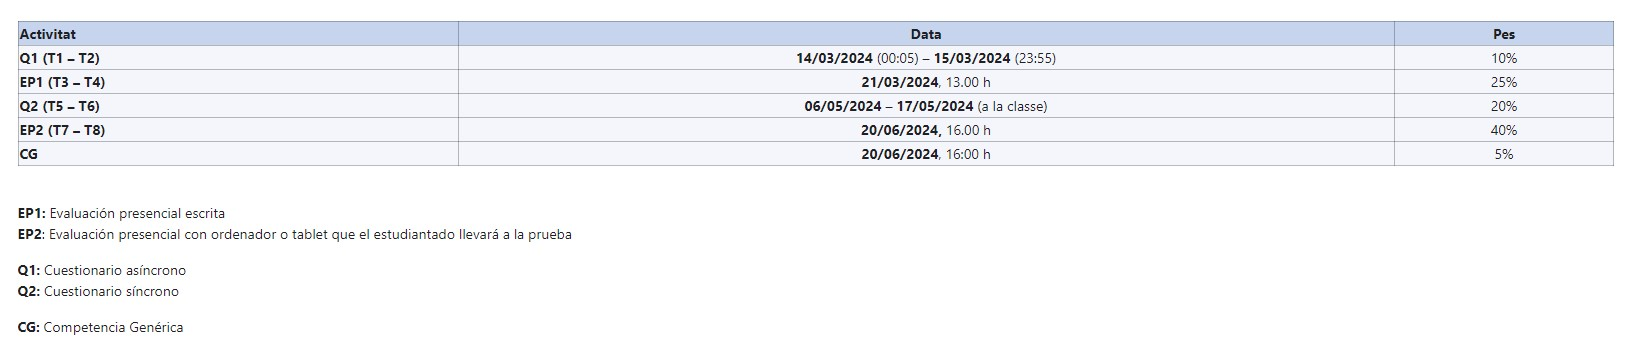
\includegraphics{./figures/notas.JPG}

Objetivos de evaluación:

\textbf{Q1} (10\%): Prueba en ordenador duración 2h en las fechas indicadas.

\begin{enumerate}
\def\labelenumi{\alph{enumi}.}
\tightlist
\item
  Dominio de comandos básicos en R (Prácticas)
\item
  Capacidad de calcular estadísticos descriptivos y gráficos, en situaciones concretas (Teoría/Práctica)
\item
  Conocimiento sobre la regresión lineal (Prácticas)
\end{enumerate}

\textbf{EP1} (25\%): Prueba escrita (2-3 problemas)

\begin{enumerate}
\def\labelenumi{\alph{enumi}.}
\tightlist
\item
  Capacidad de interpretación de enunciados en fórmulas de probabilidad (Teoría).
\item
  Conocimiento de las herramientas básicas para solucionar problemas de probabilidad conjunta y probabilidad condicional (Teoría).
\item
  Dominio matemático de funciones de probabilidad para calcular sus propiedades básicas (Teoría).
\end{enumerate}

\textbf{Q2} (20\%): Prueba en ordenador duración 2h en horario de clase en las fechas indicadas

\begin{enumerate}
\def\labelenumi{\alph{enumi}.}
\tightlist
\item
  Capacidad de identificación de modelos de probabilidad en problemas concretos (Teoría/Práctica).
\item
  Uso de funciones de R para calcular probabilidades de modelos probabilísticos (Práctica/Teoría)
\item
  Capacidad de identificación de un estadístico de muestreo y sus propiedades (Teoría/Práctica)
\item
  Conocimiento de cómo calcular la probabilidad de los estadísticos de muestreo (Teoría/Práctica)
\item
  Uso de comandos en R para calcular probabilidades y hacer simulaciones de muestras aleatorias (Prácticas)
\end{enumerate}

\textbf{EP2} (40\%): Prueba escrita (2-3 problemas)

\begin{enumerate}
\def\labelenumi{\alph{enumi}.}
\tightlist
\item
  Capacidad matemática para determinar estimadores puntuales de modelos de probabilidad.
\item
  Conociemiento de las propiedades de los estimadores puntuales.
\item
  Conocimiento de los intervalos de confianza y sus propiedades (Teoría).
\item
  Capacidad de identificar el tipo de intervalo de confianza en un problema concreto (Teoría).
\item
  Capacidad de interpretación del tipo
  de hipótesis a usar en un problema concreto (Teoría).
\item
  Uso de comandos en R para resolver problemas de intervalos de confianza y prueabas de hipótesis (Práctica).
\end{enumerate}

\textbf{CG} (5\%): Prueba escrita (2 preguntas sobre un texto)

\begin{enumerate}
\def\labelenumi{\alph{enumi}.}
\tightlist
\item
  Capacidad de expresión escrita sobre un tema relacionado a la estadística.
\end{enumerate}

coordinadores:

\begin{itemize}
\tightlist
\item
  Luis Mujica (\href{mailto:luis.eduardo.mujica@upc.edu}{\nolinkurl{luis.eduardo.mujica@upc.edu}})
\item
  Pablo Buenestado (\href{mailto:pablo.buenestado@upc.edu}{\nolinkurl{pablo.buenestado@upc.edu}})
\end{itemize}

\hypertarget{lectura-recomendada}{%
\section{Lectura recomendada}\label{lectura-recomendada}}

\begin{itemize}
\item
  Los apuntes de clase se nuestra sección estarán accesibles en ATENEA en pdf y en html.
\item
  Douglas C. Montgomery and George C. Runger. ``Applied Statistics and Probability for Engineers'' 4th Edition. Wiley 2007.
\end{itemize}

\hypertarget{descripciuxf3n-de-datos}{%
\chapter{Descripción de datos}\label{descripciuxf3n-de-datos}}

En este capítulo, presentaremos herramientas para describir datos.

Lo haremos utilizando tablas, figuras y estadísticos descriptivos de tendencia central y dispersión.

También presentaremos conceptos clave en estadística como experimentos aleatorios, observaciones, resultados y frecuencias absolutas y relativas.

\hypertarget{muxe9todo-cientuxedfico}{%
\section{Método científico}\label{muxe9todo-cientuxedfico}}

Uno de los objetivos del método científico es proporcionar un marco para resolver los problemas que surgen en el estudio de los fenómenos naturales o en el diseño de nuevas tecnologías.

Los humanos modernos han desarrollado un \textbf{método} durante miles de años que todavía está en desarrollo.

El método tiene tres actividades humanas principales:

\begin{itemize}
\tightlist
\item
  \emph{Observación} caracterizada por la adquisición de \textbf{datos}
\item
  \emph{Razón} caracterizada por el desarrollo de \textbf{modelos} matemáticos
\item
  \emph{Acción} caracterizada por el desarrollo de nuevos \textbf{experimentos} (tecnología)
\end{itemize}

Su compleja interacción y resultados son la base de la \emph{actividad científica}.

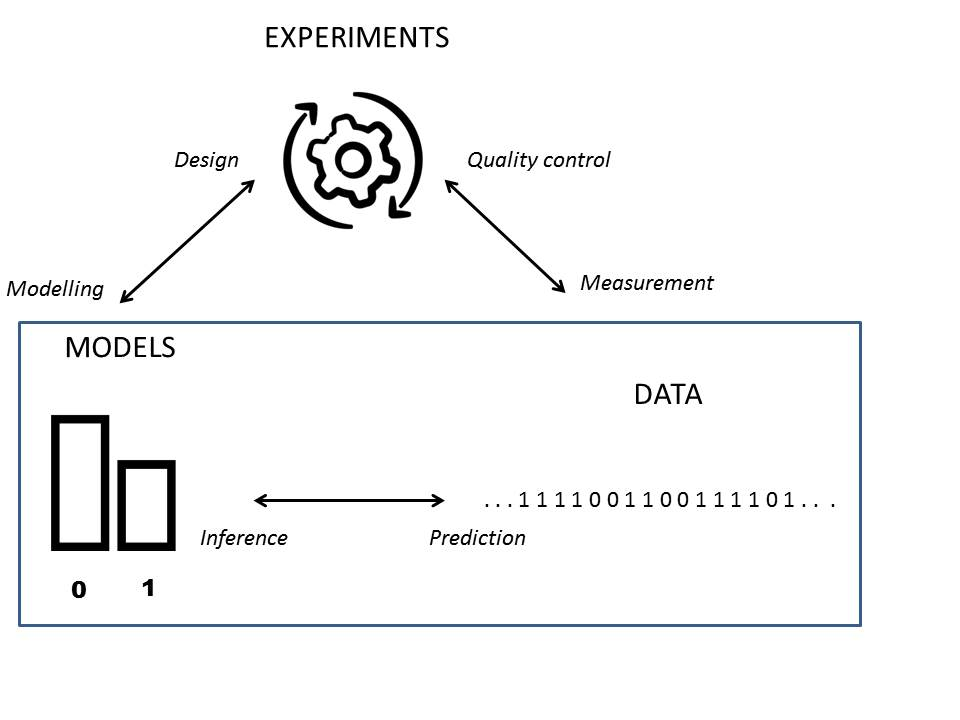
\includegraphics{./figures/stats.JPG}

\hypertarget{estaduxedstica}{%
\section{Estadística}\label{estaduxedstica}}

La estadística se ocupa de la interacción entre \emph{modelos} y \emph{datos} (la parte inferior de la figura).

Las preguntas de tipo estadístico son:

\begin{itemize}
\tightlist
\item
  ¿Cuál es el mejor modelo para mis datos (inferencia)?
\item
  ¿Cuáles son los datos que produciría un determinado modelo (predicción)?
\end{itemize}

\hypertarget{datos}{%
\section{Datos}\label{datos}}

Los datos se presentan en forma de observaciones.

Una \textbf{Observación} o \emph{Realización} es la adquisición de un número o una característica de un experimento.

Por ejemplo, tomemos la serie de números que se producen por la repetición de un experimento (1: éxito, 0: fracaso)

\ldots{} 1 0 0 1 0 \textbf{1} 0 1 1 \ldots{}

El número en negrita es \textbf{una observación} en una repetición del experimento

Un \textbf{resultado} es una \textbf{posible} observación que es el resultado de un experimento.

\textbf{1} es un resultado, \textbf{0} es el otro resultado del experimento.

Recuerda que la observación es \textbf{concreta} es el número que obtienes un día en el laboratorio. El resultado \textbf{abstracto} es una de las características del tipo de experimento que estás realizando.

\hypertarget{tipos-de-resultado}{%
\section{Tipos de resultado}\label{tipos-de-resultado}}

En estadística nos interesan principalmente dos tipos de resultados.

\begin{itemize}
\item
  \textbf{Categóricos}: Si el resultado de un experimento es una cualidad. Pueden ser nominales (binario: sí, no; múltiple: colores) u ordinales cuando las cualidades pueden jerarquizarse (gravedad de una enfermedad).
\item
  \textbf{Numéricos}: Si el resultado de un experimento es un número. El número puede ser discreto (número de correos electrónicos recibidos en una hora, número de leucocitos en sangre) o continuo (estado de carga de la batería, temperatura del motor).
\end{itemize}

\hypertarget{experimentos-aleatorios}{%
\section{Experimentos aleatorios}\label{experimentos-aleatorios}}

Se puede decir que el tema de estudio de la estadística son los experimentos aleatorios, el medio por el cual producimos datos.

\textbf{Definición:}

Un \textbf{experimento aleatorio} es un experimento que da diferentes resultados cuando se repite de la misma manera.

Los experimentos aleatorios son de diferentes tipos, dependiendo de cómo se realicen:

\begin{itemize}
\tightlist
\item
  en el mismo objeto (persona): temperatura, niveles de azúcar.
\item
  sobre objetos diferentes pero de la misma medida: el peso de un animal.
\item
  sobre eventos: el número de huracanes por año.
\end{itemize}

\hypertarget{frecuencias-absolutas}{%
\section{Frecuencias absolutas}\label{frecuencias-absolutas}}

Cuando repetimos un experimento aleatorio con resultados \textbf{categóricos}, registramos una lista de resultados.

Resumimos las observaciones contando cuántas veces vimos un resultado particular.

\textbf{Frecuencia absoluta}:

\[n_i\]

es el número de veces que observamos el resultado \(i\).

\textbf{Ejemplo (leucocitos)}

Extraigamos un leucocito de \textbf{un} donante y anotemos su tipo. Repitamos el experimento \(N=119\) veces.

\begin{verbatim}
(célula T, célula T, neutrófilo, ..., célula B)
\end{verbatim}

La segunda \textbf{célula T} en negrita es la segunda observación. La última \textbf{célula B} es la observación número 119.

Podemos listar los \textbf{resultados} (categorías) en una \textbf{tabla de frecuencia}:

\begin{verbatim}
##      outcome ni
## 1     T Cell 34
## 2     B cell 50
## 3   basophil 20
## 4   Monocyte  5
## 5 Neutrophil 10
\end{verbatim}

De la tabla, podemos decir que, por ejemplo, \(n_1=34\) es el número total de células T observadas en la repetición del experimento. También notamos que el número total de repeticiones \(N=\sum_i n_i=119\).

\hypertarget{frecuencias-relativas}{%
\section{Frecuencias relativas}\label{frecuencias-relativas}}

También podemos resumir las observaciones calculando la \textbf{proporción} de cuántas veces vimos un resultado en particular.

\[f_i=n_i/N\] donde \(N\) es el número total de observaciones

En nuestro ejemplo se registraron \(n_1=34\) células T, por lo que nos preguntamos por la proporción de células T del total de \(119\). Podemos agregar estas proporciones \(f_i\) en la tabla las frecuencias.

\begin{verbatim}
##      outcome ni         fi
## 1     T Cell 34 0.28571429
## 2     B cell 50 0.42016807
## 3   basophil 20 0.16806723
## 4   Monocyte  5 0.04201681
## 5 Neutrophil 10 0.08403361
\end{verbatim}

Las frecuencias relativas son \textbf{fundamentales} en estadística. Dan la proporción de un resultado en relación con los otros resultados. Más adelante las entenderemos como las observaciones de las probabilidades.

Para las frecuencias absolutas y relativas tenemos las propiedades

\begin{itemize}
\tightlist
\item
  \(\sum_{i=1..M} n_i = N\)
\item
  \(\sum_{i=1..M} f_i = 1\)
\end{itemize}

donde \(M\) es el número de resultados.

\hypertarget{diagrama-de-barras}{%
\section{Diagrama de barras}\label{diagrama-de-barras}}

Cuando tenemos muchos resultados y queremos ver cuáles son los más probables, podemos usar un gráfico de barras que es una cifra de \(n_i\) Vs los resultados.

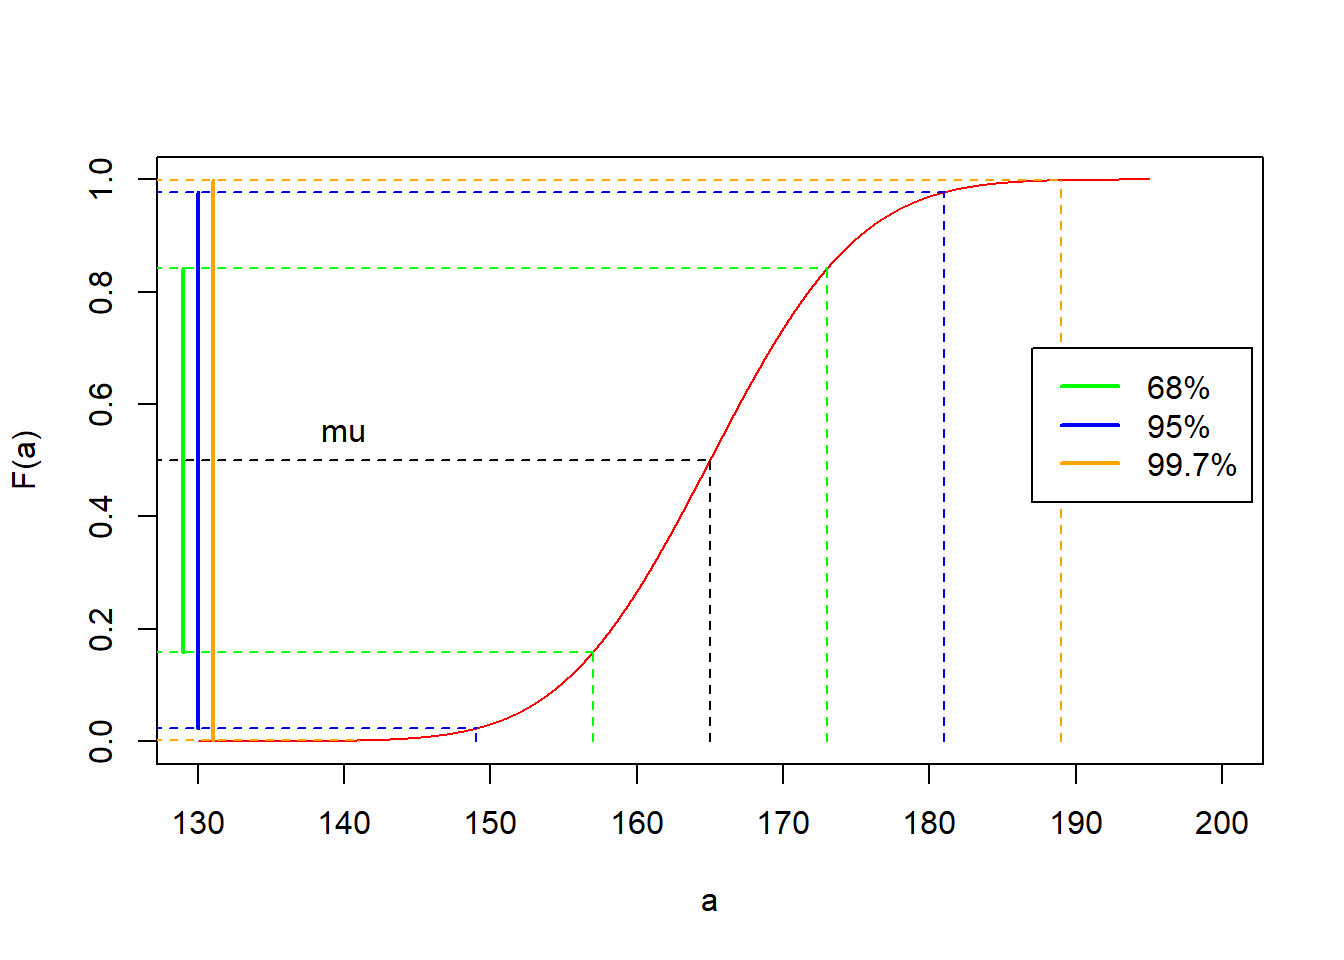
\includegraphics{_main_files/figure-latex/unnamed-chunk-3-1.pdf}

\hypertarget{gruxe1fico-de-sectores-pie}{%
\section{Gráfico de sectores (pie)}\label{gruxe1fico-de-sectores-pie}}

También podemos visualizar las frecuencias relativas con un gráfico de sectores.

El área del círculo representa el 100\% de las observaciones (proporción = 1) y las secciones las frecuencias relativas de cada resultado.

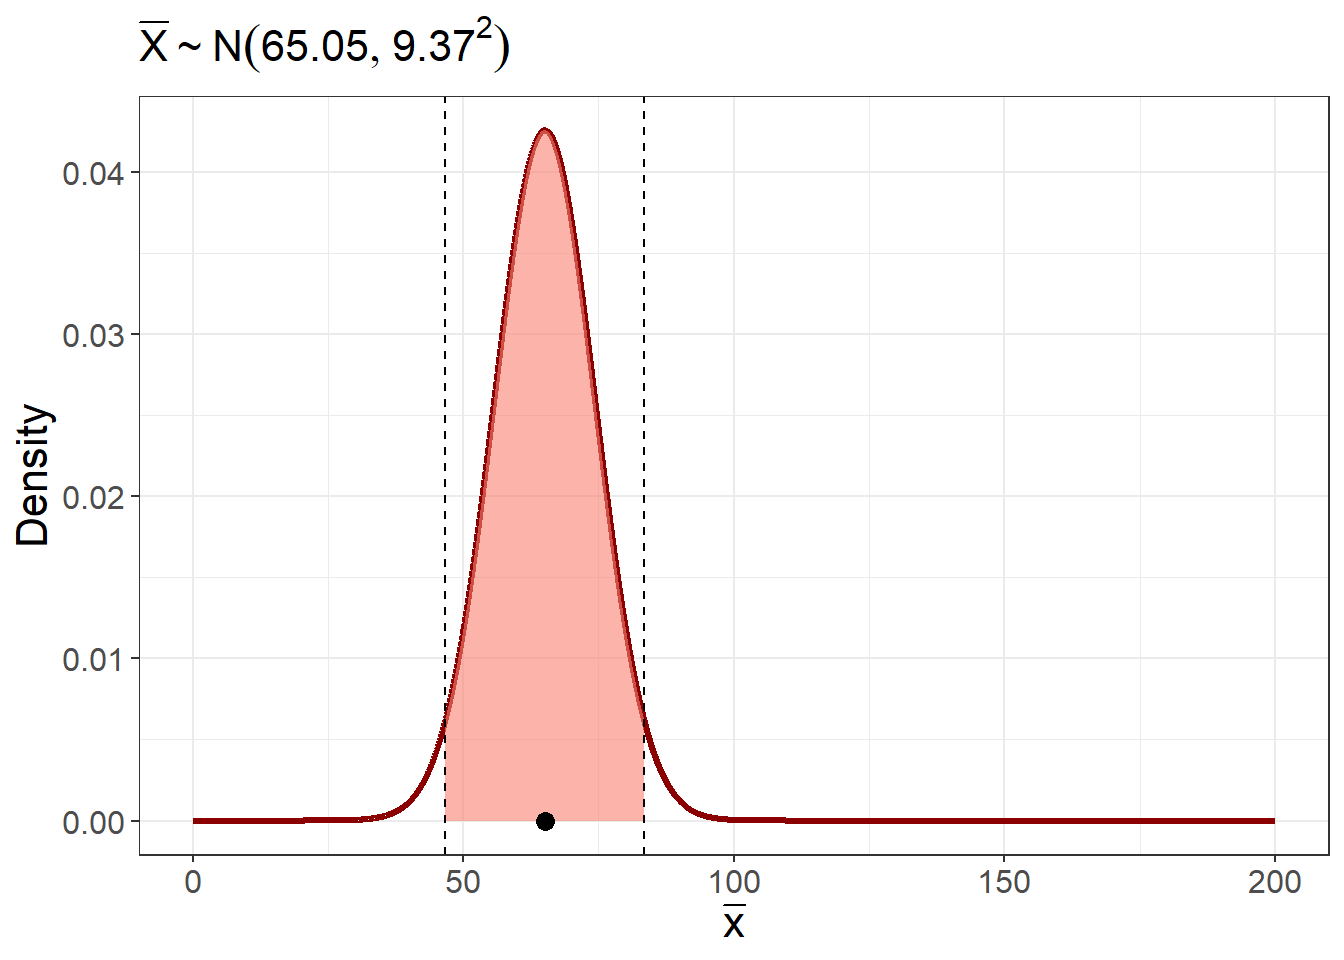
\includegraphics{_main_files/figure-latex/unnamed-chunk-4-1.pdf}

\hypertarget{variables-categuxf3ricas-ordinales}{%
\section{Variables categóricas ordinales}\label{variables-categuxf3ricas-ordinales}}

El tipo de leucocito de los ejemplos anteriores es una variable nominal \textbf{categórica}. Cada observación pertenece a una categoría (cualidad). Las categorías no siempre tienen un orden determindado.

A veces, las variables \textbf{categóricas} se pueden \textbf{ordenar} cuando cumplen una clasificación natural. Esto permite introducir \textbf{frecuencias acumulativas}.

\textbf{Ejemplo (misofonía)}

Este es un estudio clínico en 123 pacientes que fueron examinados por su grado de misofonía. La misofnía es ansiedad/ira descontrolada producida por ciertos sonidos.

Cada paciente fue evaluado con un cuestionario (AMISO) y se clasificaron en 4 grupos diferentes según la gravedad.

Los resultados del estudio son

\begin{verbatim}
##   [1] 4 2 0 3 0 0 2 3 0 3 0 2 2 0 2 0 0 3 3 0 3 3 2 0 0 0 4 2 2 0 2 0 0 0 3 0 2
##  [38] 3 2 2 0 2 3 0 0 2 2 3 3 0 0 4 3 3 2 0 2 0 0 0 2 2 0 0 2 3 0 1 3 2 4 3 2 3
##  [75] 0 2 3 2 4 1 2 0 2 0 2 0 2 2 4 3 0 3 0 0 0 2 2 1 3 0 0 3 2 1 3 0 4 4 2 3 3
## [112] 3 0 3 2 1 2 3 3 4 2 3 2
\end{verbatim}

Cada observación es el resultado de un experimento aleatorio: medición del nivel de misofonía en un paciente. Esta serie de datos se puede resumir en términos de los resultados en la tabla de frecuencia

\begin{verbatim}
##   outcome ni         fi
## 1       0 41 0.33333333
## 2       1  5 0.04065041
## 3       2 37 0.30081301
## 4       3 31 0.25203252
## 5       4  9 0.07317073
\end{verbatim}

\hypertarget{frecuencias-acumuladas-absolutas-y-relativas}{%
\section{Frecuencias acumuladas absolutas y relativas}\label{frecuencias-acumuladas-absolutas-y-relativas}}

La gravedad de la misofonía es \textbf{categórica} \textbf{ordinal} porque sus resultados pueden ordenarse en relación con su grado.

Cuando los resultados se pueden ordenar, es útil preguntar cuántas observaciones se obtuvieron hasta un resultado dado. Llamamos a este número la \textbf{frecuencia acumulada absoluta} hasta el resultado \(i\):
\[N_i=\sum_{k=1..i} n_k\]
También es útil para calcular la \textbf{proporción} de las observaciones que se obtuvo hasta un resultado dado

\[F_i=\sum_{k=1..i} f_k\]

Podemos agregar estas frecuencias en la \textbf{tabla de frecuencias}

\begin{verbatim}
##   outcome ni         fi  Ni        Fi
## 0       0 41 0.33333333  41 0.3333333
## 1       1  5 0.04065041  46 0.3739837
## 2       2 37 0.30081301  83 0.6747967
## 3       3 31 0.25203252 114 0.9268293
## 4       4  9 0.07317073 123 1.0000000
\end{verbatim}

Por lo tanto, el \textbf{67 \%} de los pacientes tenían misofonía hasta la gravedad \textbf{2} y el \textbf{37 \%} de los pacientes tenían una gravedad inferior o igual a \textbf{1}.

\hypertarget{gruxe1fica-de-frecuencia-acumulada}{%
\section{Gráfica de frecuencia acumulada}\label{gruxe1fica-de-frecuencia-acumulada}}

\(F_i\) es una cantidad importante porque nos permite definir la acumulación de probabilidades hasta niveles intermedios.

La probabilidad de un nivel intermedio \(x\) (\(i\leq x< i+1\)) es solo la acumulación hasta el nivel inferior \(F_x=F_i\).

\(F_x\) es por lo tanto una función de rango \textbf{continuo}. Podemos dibujarla con respecto a los resultados.

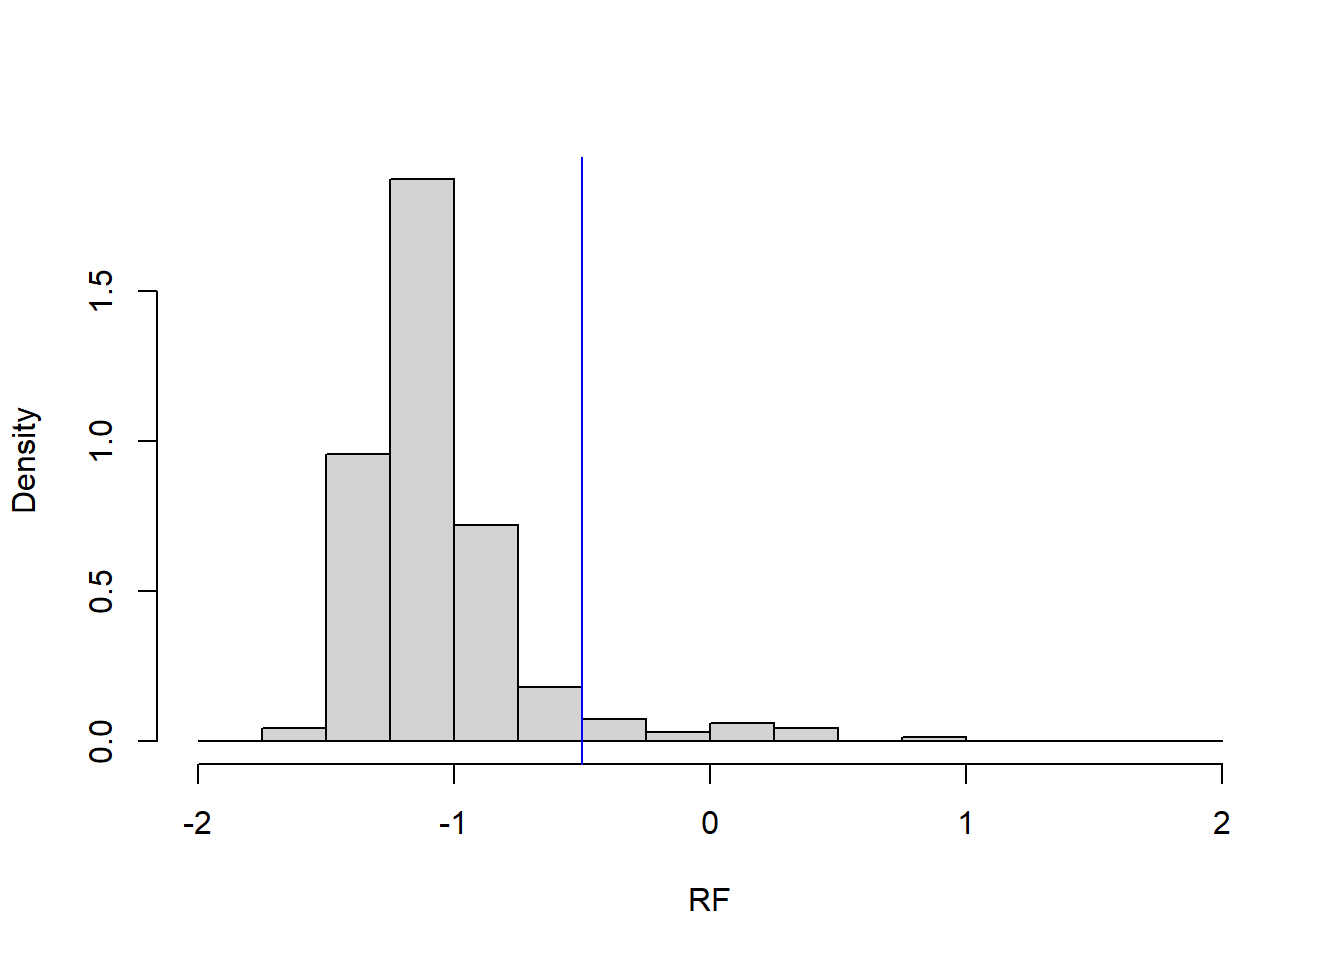
\includegraphics{_main_files/figure-latex/unnamed-chunk-8-1.pdf}

Por lo tanto, podemos decir que el \textbf{67 \%} de los pacientes tenían misofonía hasta gravedad \(2.3\), aunque \(2.3\) no es un resultado observado.

\hypertarget{variables-numuxe9ricas}{%
\section{Variables numéricas}\label{variables-numuxe9ricas}}

El resultado de un experimento aleatorio puede producir un número. Si el número es \textbf{discreto}, podemos generar una tabla de frecuencias, con frecuencias absolutas, relativas y acumulativas, e ilustrarlas con gráficos de barras, de sectores y acumulativos.

Cuando el número es \textbf{continuo} las frecuencias no son útiles, lo más probable es que observemos o no un número contínuo en particular.

\textbf{Ejemplo (misofonía)}

Los investigadores se preguntaron si la convexidad de la mandíbula afectaría la gravedad de la misofonía. La hipótesis científica es que el ángulo de convexidad de la mandíbula puede influir en el oído y su sensibilidad. Estos son los resultados de la convexidad de la mandíbula (grados) para cada paciente:

\begin{verbatim}
##   [1]  7.97 18.23 12.27  7.81  9.81 13.50 19.30  7.70 12.30  7.90 12.60 19.00
##  [13]  7.27 14.00  5.40  8.00 11.20  7.75  7.94 16.69  7.62  7.02  7.00 19.20
##  [25]  7.96 14.70  7.24  7.80  7.90  4.70  4.40 14.00 14.40 16.00  1.40  9.76
##  [37]  7.90  7.90  7.40  6.30  7.76  7.30  7.00 11.23 16.00  7.90  7.29  6.91
##  [49]  7.10 13.40 11.60 -1.00  6.00  7.82  4.80 11.00  9.00 11.50 16.00 15.00
##  [61]  1.40 16.80  7.70 16.14  7.12 -1.00 17.00  9.26 18.70  3.40 21.30  7.50
##  [73]  6.03  7.50 19.00 19.01  8.10  7.80  6.10 15.26  7.95 18.00  4.60 15.00
##  [85]  7.50  8.00 16.80  8.54  7.00 18.30  7.80 16.00 14.00 12.30 11.40  8.50
##  [97]  7.00  7.96 17.60 10.00  3.50  6.70 17.00 20.26  6.64  1.80  7.02  2.46
## [109] 19.00 17.86  6.10  6.64 12.00  6.60  8.70 14.05  7.20 19.70  7.70  6.02
## [121]  2.50 19.00  6.80
\end{verbatim}

\hypertarget{transformando-datos-continuos}{%
\section{Transformando datos continuos}\label{transformando-datos-continuos}}

Como los resultados continuos no se pueden contar (de manera informativa), los transformamos en variables categóricas ordenadas.

\begin{enumerate}
\def\labelenumi{\arabic{enumi})}
\tightlist
\item
  Primero cubrimos el rango de las observaciones en intervalos regulares del mismo tamaño (contenedores)
\end{enumerate}

\begin{verbatim}
## [1] "[-1.02,3.46]" "(3.46,7.92]"  "(7.92,12.4]"  "(12.4,16.8]"  "(16.8,21.3]"
\end{verbatim}

\begin{enumerate}
\def\labelenumi{\arabic{enumi})}
\setcounter{enumi}{1}
\tightlist
\item
  Luego mapeamos cada observación a su intervalo: creando una variable categórica \textbf{ordenada}; en este caso con 5 resultados posibles
\end{enumerate}

\begin{verbatim}
##   [1] "(7.92,12.4]"  "(16.8,21.3]"  "(7.92,12.4]"  "(3.46,7.92]"  "(7.92,12.4]" 
##   [6] "(12.4,16.8]"  "(16.8,21.3]"  "(3.46,7.92]"  "(7.92,12.4]"  "(3.46,7.92]" 
##  [11] "(12.4,16.8]"  "(16.8,21.3]"  "(3.46,7.92]"  "(12.4,16.8]"  "(3.46,7.92]" 
##  [16] "(7.92,12.4]"  "(7.92,12.4]"  "(3.46,7.92]"  "(7.92,12.4]"  "(12.4,16.8]" 
##  [21] "(3.46,7.92]"  "(3.46,7.92]"  "(3.46,7.92]"  "(16.8,21.3]"  "(7.92,12.4]" 
##  [26] "(12.4,16.8]"  "(3.46,7.92]"  "(3.46,7.92]"  "(3.46,7.92]"  "(3.46,7.92]" 
##  [31] "(3.46,7.92]"  "(12.4,16.8]"  "(12.4,16.8]"  "(12.4,16.8]"  "[-1.02,3.46]"
##  [36] "(7.92,12.4]"  "(3.46,7.92]"  "(3.46,7.92]"  "(3.46,7.92]"  "(3.46,7.92]" 
##  [41] "(3.46,7.92]"  "(3.46,7.92]"  "(3.46,7.92]"  "(7.92,12.4]"  "(12.4,16.8]" 
##  [46] "(3.46,7.92]"  "(3.46,7.92]"  "(3.46,7.92]"  "(3.46,7.92]"  "(12.4,16.8]" 
##  [51] "(7.92,12.4]"  "[-1.02,3.46]" "(3.46,7.92]"  "(3.46,7.92]"  "(3.46,7.92]" 
##  [56] "(7.92,12.4]"  "(7.92,12.4]"  "(7.92,12.4]"  "(12.4,16.8]"  "(12.4,16.8]" 
##  [61] "[-1.02,3.46]" "(12.4,16.8]"  "(3.46,7.92]"  "(12.4,16.8]"  "(3.46,7.92]" 
##  [66] "[-1.02,3.46]" "(16.8,21.3]"  "(7.92,12.4]"  "(16.8,21.3]"  "[-1.02,3.46]"
##  [71] "(16.8,21.3]"  "(3.46,7.92]"  "(3.46,7.92]"  "(3.46,7.92]"  "(16.8,21.3]" 
##  [76] "(16.8,21.3]"  "(7.92,12.4]"  "(3.46,7.92]"  "(3.46,7.92]"  "(12.4,16.8]" 
##  [81] "(7.92,12.4]"  "(16.8,21.3]"  "(3.46,7.92]"  "(12.4,16.8]"  "(3.46,7.92]" 
##  [86] "(7.92,12.4]"  "(12.4,16.8]"  "(7.92,12.4]"  "(3.46,7.92]"  "(16.8,21.3]" 
##  [91] "(3.46,7.92]"  "(12.4,16.8]"  "(12.4,16.8]"  "(7.92,12.4]"  "(7.92,12.4]" 
##  [96] "(7.92,12.4]"  "(3.46,7.92]"  "(7.92,12.4]"  "(16.8,21.3]"  "(7.92,12.4]" 
## [101] "(3.46,7.92]"  "(3.46,7.92]"  "(16.8,21.3]"  "(16.8,21.3]"  "(3.46,7.92]" 
## [106] "[-1.02,3.46]" "(3.46,7.92]"  "[-1.02,3.46]" "(16.8,21.3]"  "(16.8,21.3]" 
## [111] "(3.46,7.92]"  "(3.46,7.92]"  "(7.92,12.4]"  "(3.46,7.92]"  "(7.92,12.4]" 
## [116] "(12.4,16.8]"  "(3.46,7.92]"  "(16.8,21.3]"  "(3.46,7.92]"  "(3.46,7.92]" 
## [121] "[-1.02,3.46]" "(16.8,21.3]"  "(3.46,7.92]"
\end{verbatim}

Por tanto, en lugar de decir que el primer paciente tenía un ángulo de convexidad de \(7.97\), decimos que su ángulo estaba entre el intervalo (o \textbf{bin}) \((7.92,12.4]\).

Ningún otro paciente tenía un ángulo de \(7.97\), pero muchos tenían ángulos entre \((7.92,12.4]\).

\hypertarget{tabla-de-frecuencias-para-una-variable-continua}{%
\section{Tabla de frecuencias para una variable continua}\label{tabla-de-frecuencias-para-una-variable-continua}}

Para una partición regular dada del intervalo de resultados en intervalos, podemos producir una tabla de frecuencias como antes

\begin{verbatim}
##        outcome ni         fi  Ni         Fi
## 1 [-1.02,3.46]  8 0.06504065   8 0.06504065
## 2  (3.46,7.92] 51 0.41463415  59 0.47967480
## 3  (7.92,12.4] 26 0.21138211  85 0.69105691
## 4  (12.4,16.8] 20 0.16260163 105 0.85365854
## 5  (16.8,21.3] 18 0.14634146 123 1.00000000
\end{verbatim}

\hypertarget{histograma}{%
\section{Histograma}\label{histograma}}

El histograma es la gráfica de \(n_i\) o \(f_i\) Vs los resultados en intervalos (bins). El histograma depende del tamaño de los bins.

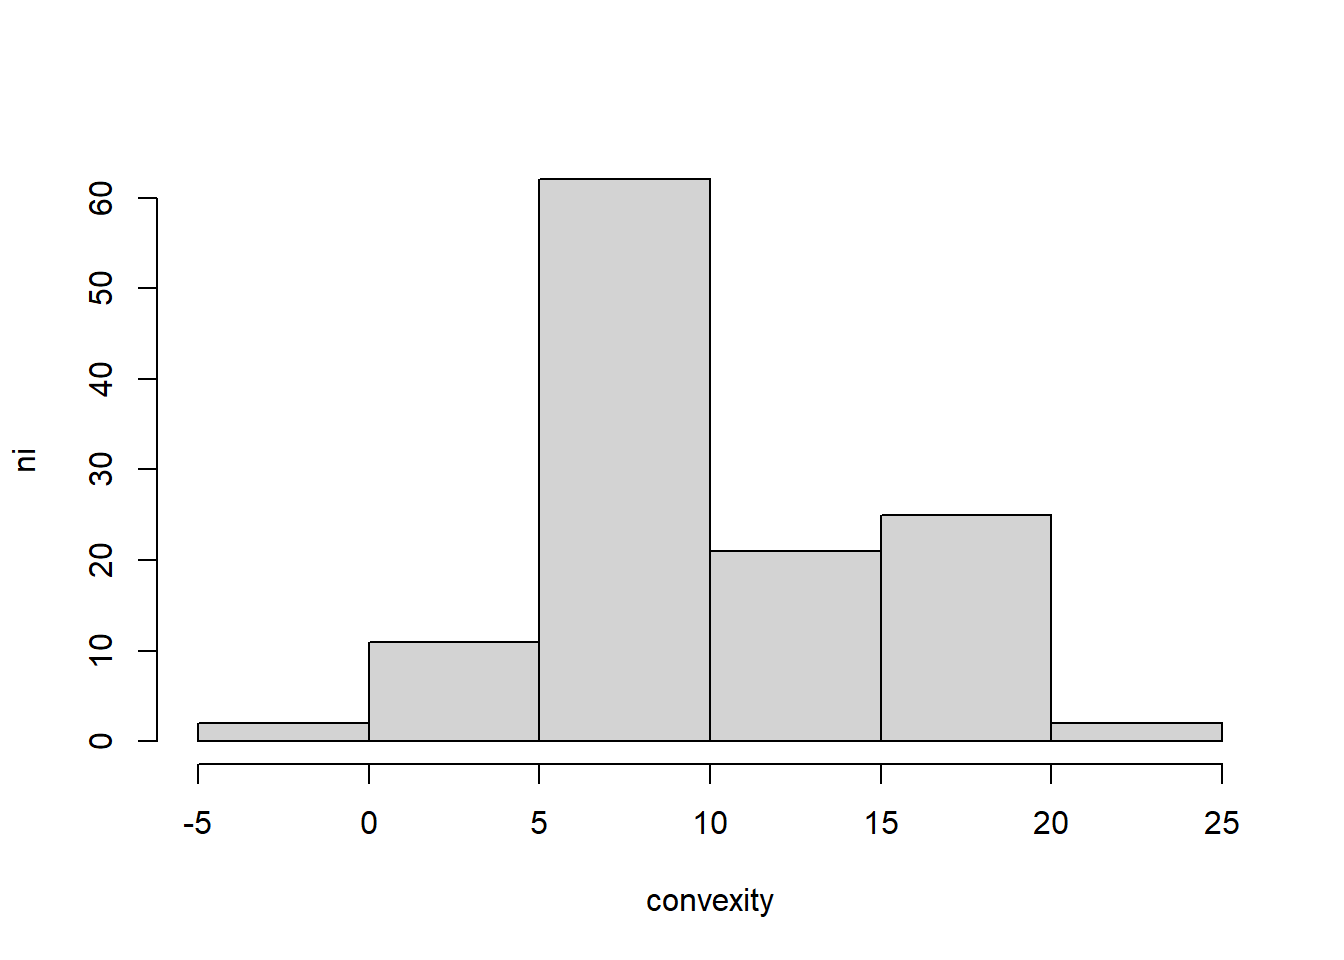
\includegraphics{_main_files/figure-latex/unnamed-chunk-13-1.pdf}

Este es un histograma con 20 bins.

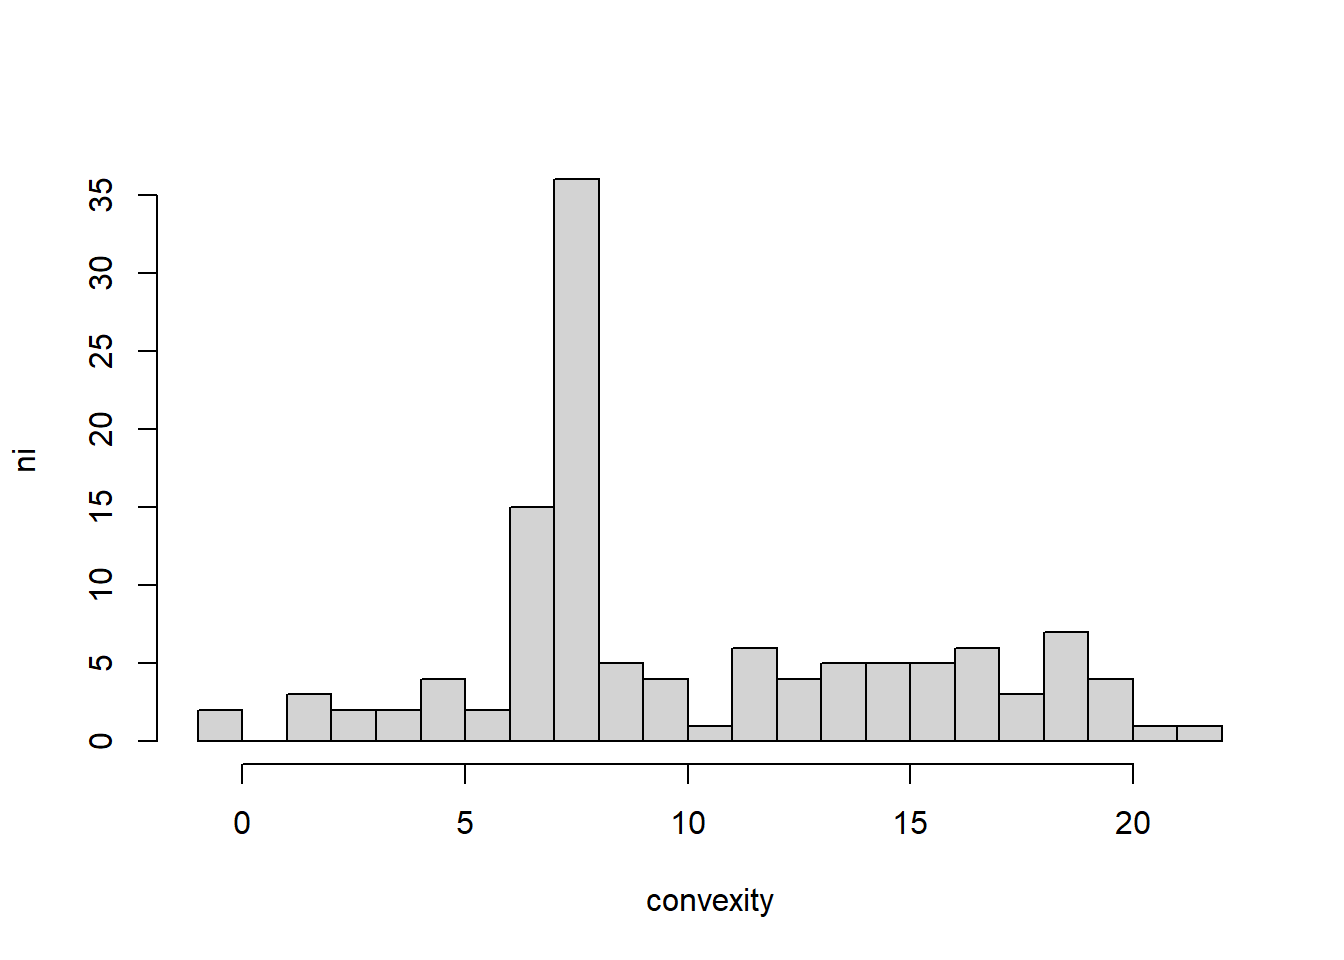
\includegraphics{_main_files/figure-latex/unnamed-chunk-14-1.pdf}

Vemos que la mayoría de las personas tienen ángulos dentro de \((7, 8]\)

\hypertarget{gruxe1fica-de-frecuencia-acumulada-1}{%
\section{Gráfica de frecuencia acumulada}\label{gruxe1fica-de-frecuencia-acumulada-1}}

También podemos graficar \(F_x\) contra los resultados. Como \(F_x\) es de rango continuo, podemos ordenar las observaciones (\(x_1 <... x_j < x_{j+1} < x_n\)) y por lo tanto

\[F_x = \frac{k}{n}\]

para \(x_{k} \leq x < x_{k+1}\).

\(F_x\) se conoce como la \textbf{distribución} de los datos. \(F_x\) no depende del tamaño del bin. Sin embargo, su \textbf{resolución} depende de la cantidad de datos.

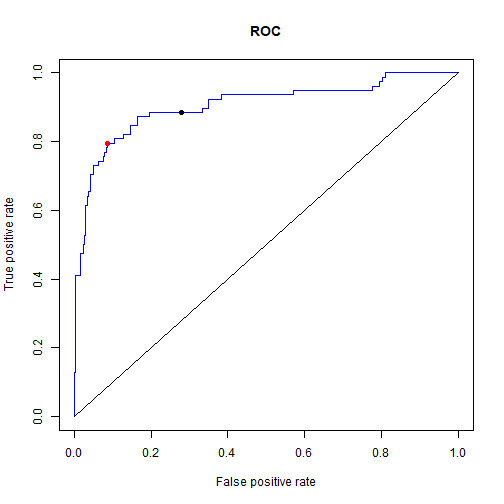
\includegraphics{_main_files/figure-latex/unnamed-chunk-15-1.pdf}

\hypertarget{estaduxedsticas-de-resumen}{%
\section{Estadísticas de resumen}\label{estaduxedsticas-de-resumen}}

Las estadísticas de resumen son números calculados a partir de los datos que nos dicen características importantes de las variables numéricas (discretas o continuas).

Por ejemplo, tenemos estadísticas que describen los valores extremos:

\begin{itemize}
\tightlist
\item
  \textbf{mínimo}: el resultado mínimo observado
\item
  \textbf{máximo}: el resultado máximo observado
\end{itemize}

\hypertarget{promedio-media-muestral}{%
\section{Promedio (media muestral)}\label{promedio-media-muestral}}

Una estadística importante que describe el valor central de los resultados (dónde esperar la mayoría de las observaciones) es el \textbf{promedio}

\[\bar{x}=\frac{1}{N} \sum_{j=1..N} x_j\]

donde \(x_j\) es la \textbf{observación} \(j\) de un total de \(N\).

\textbf{Ejemplo (Misofonía)}

La convexidad promedio se puede calcular directamente a partir de las \textbf{observaciones}

\(\bar{x}= \frac{1}{N}\sum_j x_j\)

\(= \frac{1}{N}(7.97 + 18.23 + 12.27... + 6.80) = 10.19894\)

Para variables \textbf{categóricamente ordenadas}, podemos usar las frecuencias relativas para calcular el promedio

\(\bar{x}=\frac{1}{N}\sum_{i=1...N} x_j=\frac{1}{N}\sum_{i=1...M} x_i*n_ {i}\)
\[=\sum_{i=1...M} x_i*f_{i}\]

donde pasamos de sumar \(N\) \textbf{observaciones} a sumar \(M\) \textbf{resultados}.

La forma \(\bar{x}= \sum_{i = 1...M} x_i f_i\) muestra que el promedio es el \textbf{centro de gravedad} de los resultados. Como si cada resultado tuviera una densidad de masa dada por \(f_i\).

\textbf{Ejemplo (Misofonía)}

La \textbf{severidad} promedio de la misofonía en el estudio se puede calcular a partir de las frecuencias relativas de los \textbf{resultados}

\begin{verbatim}
##   outcome ni         fi
## 1       0 41 0.33333333
## 2       1  5 0.04065041
## 3       2 37 0.30081301
## 4       3 31 0.25203252
## 5       4  9 0.07317073
\end{verbatim}

\(\bar{x}=0*f_{0}+1*f_{1}+2*f_{2}+3*f_{3}+4*f_{4}=1.691057\)

\hypertarget{promedio}{%
\section{Promedio}\label{promedio}}

El promedio es también el centro de gravedad de las variables continuas. Ese es el punto donde las frecuencias reativas se equilibran.

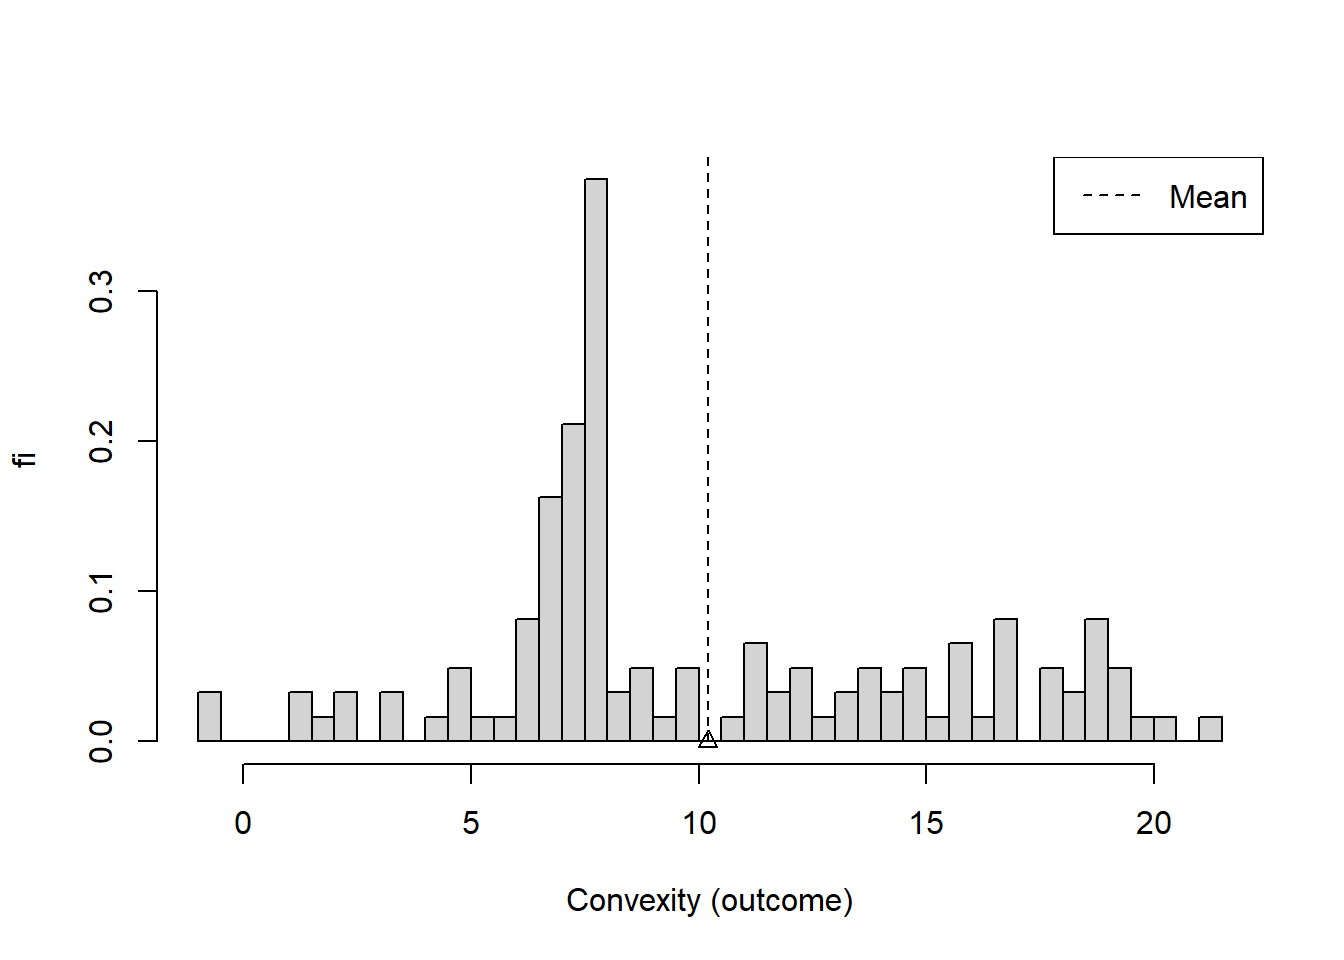
\includegraphics{_main_files/figure-latex/unnamed-chunk-17-1.pdf}

\hypertarget{mediana}{%
\section{mediana}\label{mediana}}

Otra medida de centralidad es la mediana. La mediana \(x_m\), o \(q_{0.5}\), es el valor por debajo del cual encontramos la mitad de las observaciones. Cuando ordenamos las observaciones \(x_1 <... x_j < x_{j+1} < x_N\), las contamos hasta encontrar la mitad de ellas. \(x_m\) es tal que

\[\sum_{i\leq m} 1 = \frac{N}{2}\]
\textbf{Ejemplo (Misofonía)}

Si ordenamos los ángulos de convexidad, vemos que \(62\) observaciones (individuos) (\(N/2 \sim 123/2\)) están por debajo de \(7.96\). La \textbf{convexidad mediana} es por lo tanto \(q_{0.5}=x_{62}=7.96\)

\begin{verbatim}
##  [1] -1.00 -1.00  1.40  1.40  1.80  2.46  2.50  3.40  3.50  4.40  4.60  4.70
## [13]  4.80  5.40  6.00  6.02  6.03  6.10  6.10  6.30  6.60  6.64  6.64  6.70
## [25]  6.80  6.91  7.00  7.00  7.00  7.00  7.02  7.02  7.10  7.12  7.20  7.24
## [37]  7.27  7.29  7.30  7.40  7.50  7.50  7.50  7.62  7.70  7.70  7.70  7.75
## [49]  7.76  7.80  7.80  7.80  7.81  7.82  7.90  7.90  7.90  7.90  7.90  7.94
## [61]  7.95  7.96
\end{verbatim}

\begin{verbatim}
##  [1]  7.96  7.97  8.00  8.00  8.10  8.50  8.54  8.70  9.00  9.26  9.76  9.81
## [13] 10.00 11.00 11.20 11.23 11.40 11.50 11.60 12.00 12.27 12.30 12.30 12.60
## [25] 13.40 13.50 14.00 14.00 14.00 14.05 14.40 14.70 15.00 15.00 15.26 16.00
## [37] 16.00 16.00 16.00 16.14 16.69 16.80 16.80 17.00 17.00 17.60 17.86 18.00
## [49] 18.23 18.30 18.70 19.00 19.00 19.00 19.00 19.01 19.20 19.30 19.70 20.26
## [61] 21.30
\end{verbatim}

\begin{verbatim}
## [1] 7.96
\end{verbatim}

En términos de frecuencias, \(q_{0.5}\) hace que la frecuencia acumulada \(F_x\) sea igual a \(0.5\)

\[\sum_{i = 0, ... m} f_i =F_{q_{0.5}}=0.5\]
o

\[q_{0.5}=F^{-1}(0.5)\]

En el gráfico de distribución, la mediana es el valor de \(x\) en el que se encuentra la mitad del máximo de \(F\).

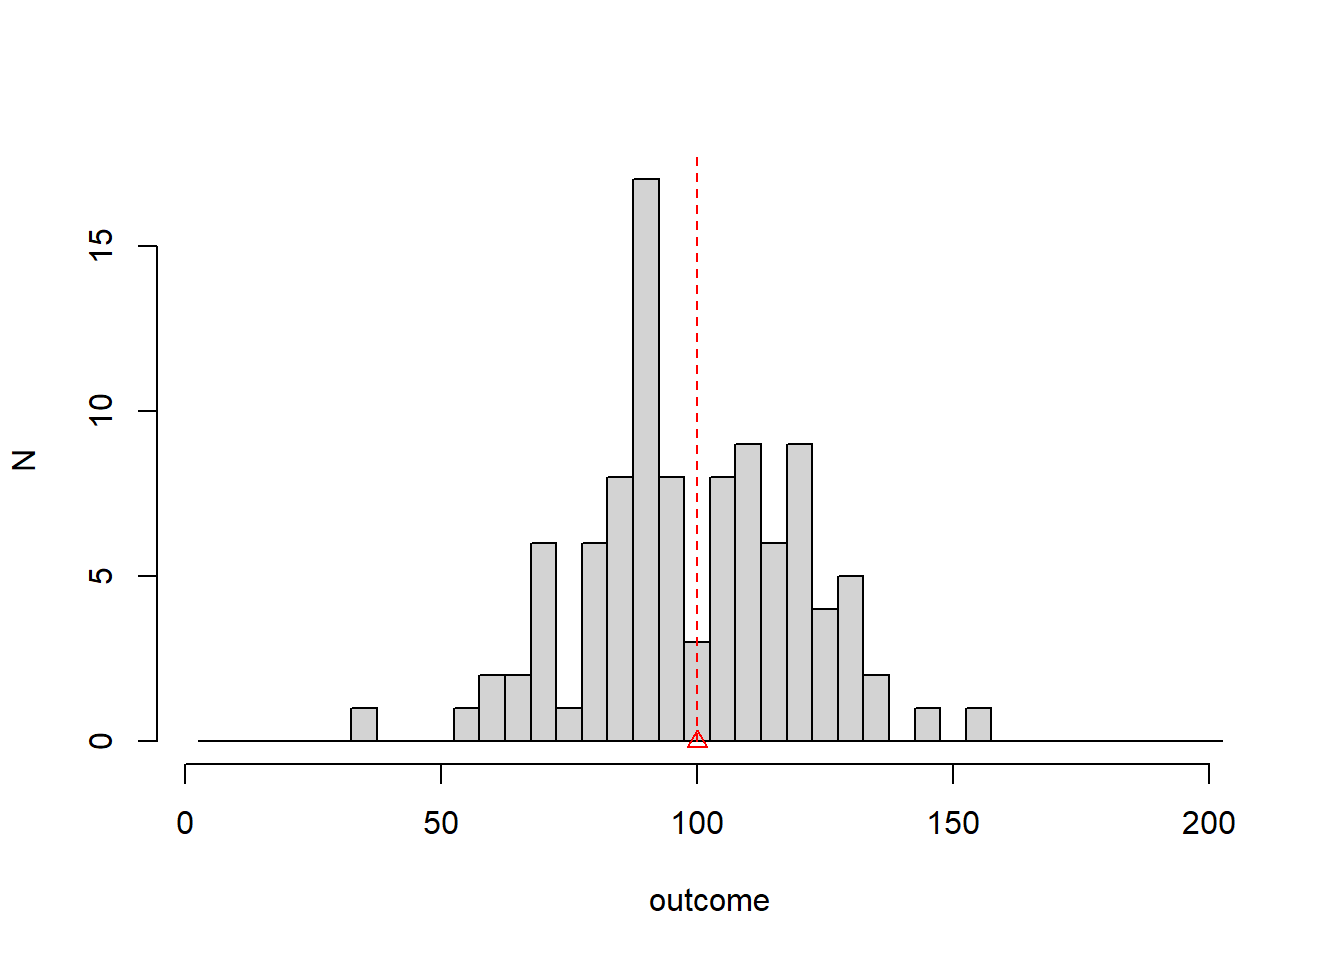
\includegraphics{_main_files/figure-latex/unnamed-chunk-20-1.pdf}

El promedio y la mediana no siempre son iguales.

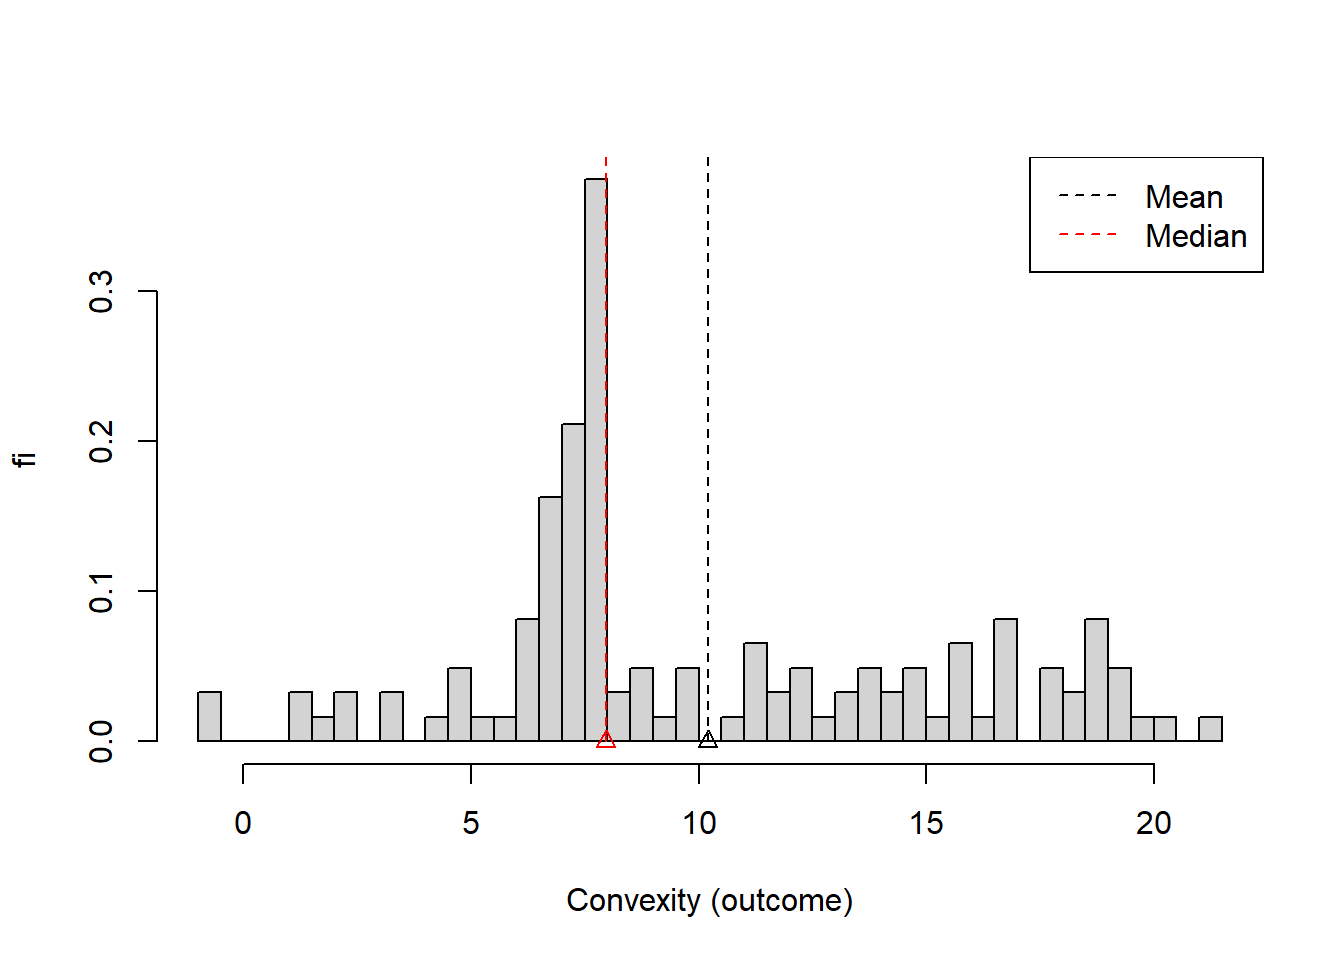
\includegraphics{_main_files/figure-latex/unnamed-chunk-21-1.pdf}

\hypertarget{dispersiuxf3n}{%
\section{Dispersión}\label{dispersiuxf3n}}

Otras estadísticas de resumen importantes de las observaciones son las de \textbf{dispersión}.

Muchos experimentos pueden compartir su media, pero difieren en cuán \textbf{dispersos} son los valores.

La dispersión de las observaciones es una medida del \textbf{ruido}.

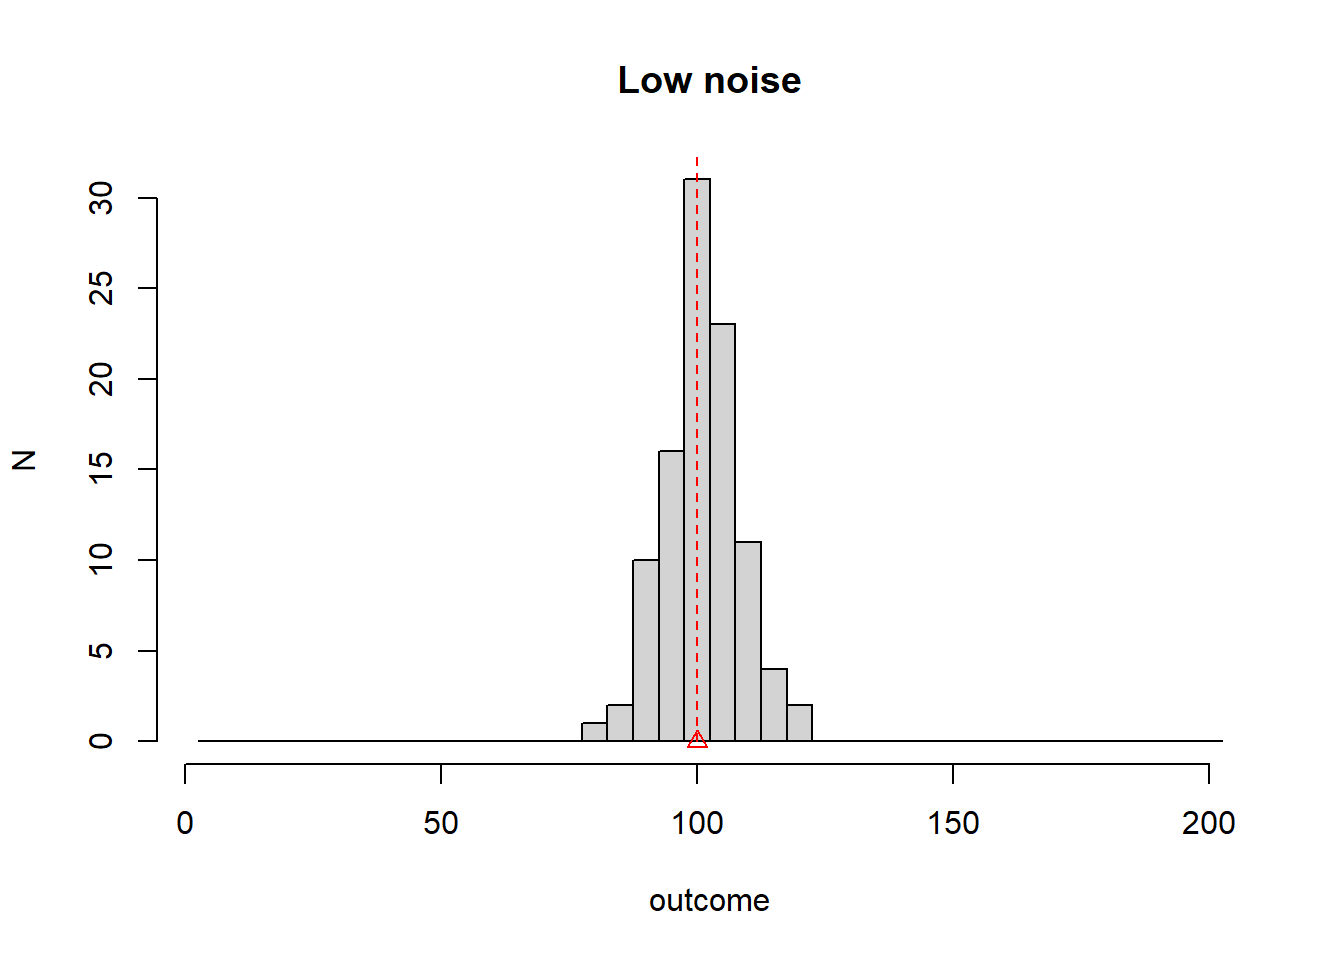
\includegraphics{_main_files/figure-latex/unnamed-chunk-22-1.pdf} 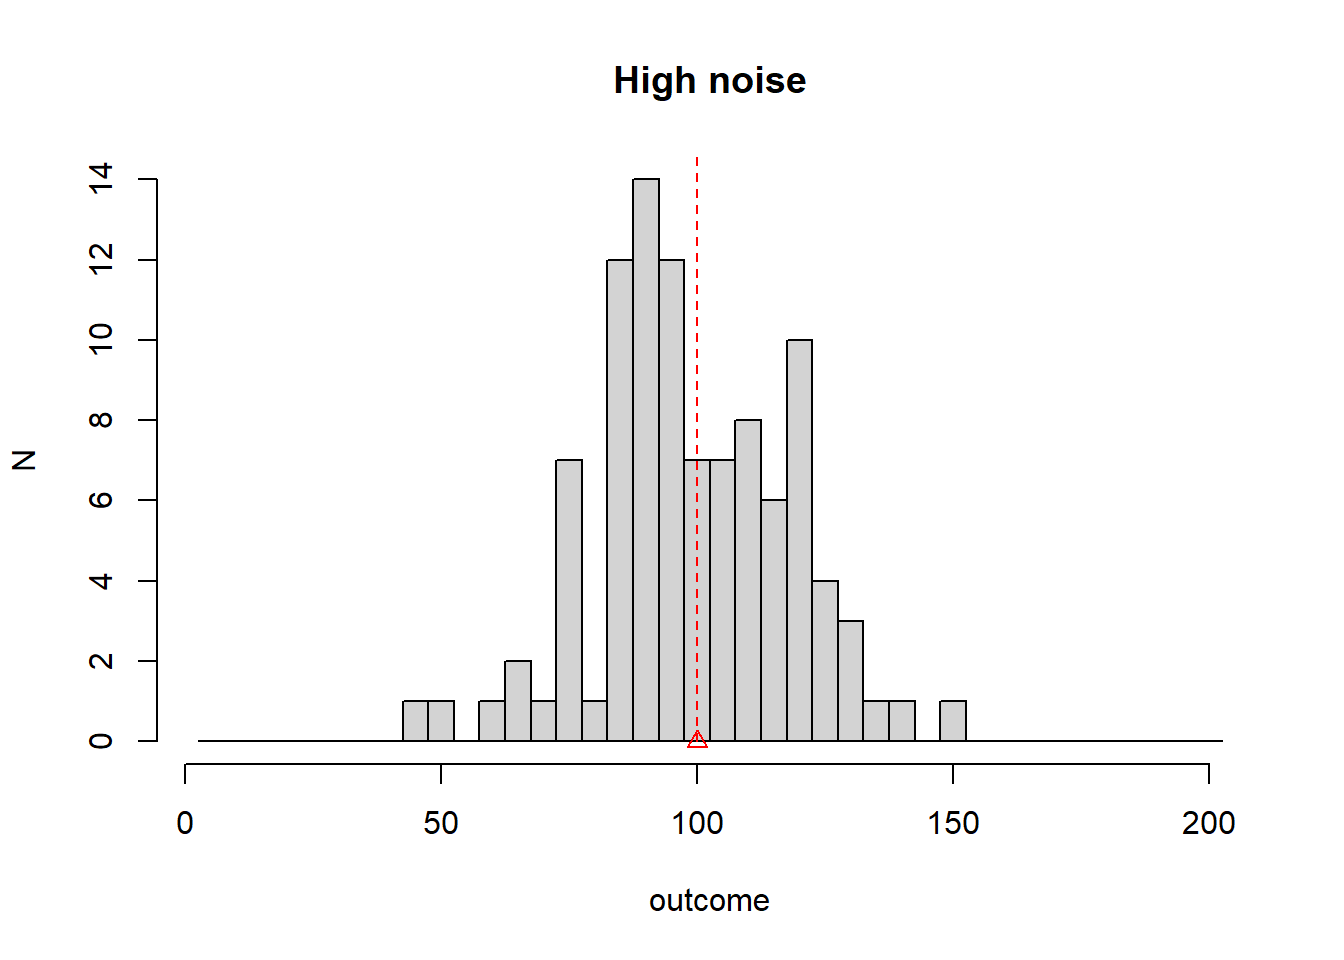
\includegraphics{_main_files/figure-latex/unnamed-chunk-22-2.pdf}

\hypertarget{variaciuxf3n-de-la-muestra}{%
\section{Variación de la muestra}\label{variaciuxf3n-de-la-muestra}}

La dispersión sobre la media se mide con la varianza muestral

\[s^2=\frac{1}{N-1} \sum_{j=1..N} (x_j-\bar{x})^2\]

Este número, mide la distancia cuadrada promedio de las \textbf{observaciones} al promedio. La razón de \(N-1\) se explicará cuando hablemos de inferencia, cuando estudiemos la dispersión de \(\bar{x}\), además de la dispersión de las observaciones.

En términos de las frecuencias de las variables \textbf{categóricas y ordenadas}

\[s^2=\frac{N}{N-1} \sum_{i=1... M} (x_i-\bar{x})^2 f_i\]

\(s^2\) se puede considerar como el \textbf{momento de inercia} de las observaciones.

La raíz cuadrada de la varianza de la muestra se denomina \textbf{desviación estándar} \(s\).

\textbf{Ejemplo (Misofonía)}

La desviación estándar del ángulo de convexidad es

\(s= [\frac{1}{123-1}((7.97-10.19894)^2+ (18.23-10.19894)^2\)
\(+ (12.27-10.19894)^2 + ...)]^{1/2} = 5.086707\)

La convexidad de la mandíbula se desvía de su media en \(5.086707\).

\hypertarget{rango-intercuartuxedlico-iqr}{%
\section{Rango intercuartílico (IQR)}\label{rango-intercuartuxedlico-iqr}}

La dispersión de los datos también se puede medir con respecto a la mediana usando el \textbf{rango intercuartílico}:

\begin{enumerate}
\def\labelenumi{\arabic{enumi})}
\tightlist
\item
  Definimos el \textbf{primer} cuartil como el valor \(x_m\) que hace que la frecuencia acumulada \(F_{q_{0.25}}\) sea igual a \(0.25\) (\(x\) donde hemos acumulado una cuarta parte de las observaciones)
\end{enumerate}

\[F_{q_{0.25}}=0.25\]

\begin{enumerate}
\def\labelenumi{\arabic{enumi})}
\tightlist
\item
  Definimos el \textbf{tercer} cuartil como el valor \(x_m\) que hace que la frecuencia acumulada \(F_{q_{0.75}}\) sea igual a \(0.75\) (\(x\) donde hemos acumulado tres cuartos de observaciones)
\end{enumerate}

\[F_{q_{0.75}}=0.75\]

\begin{enumerate}
\def\labelenumi{\arabic{enumi})}
\setcounter{enumi}{2}
\tightlist
\item
  El \textbf{rango intercuartílico} (IQR) es \(IQR=q_{0.75} - q_{0.25}\). Esa es la distancia entre el tercer y el primer cuartil y captura el \(50\%\) central de las observaciones
\end{enumerate}

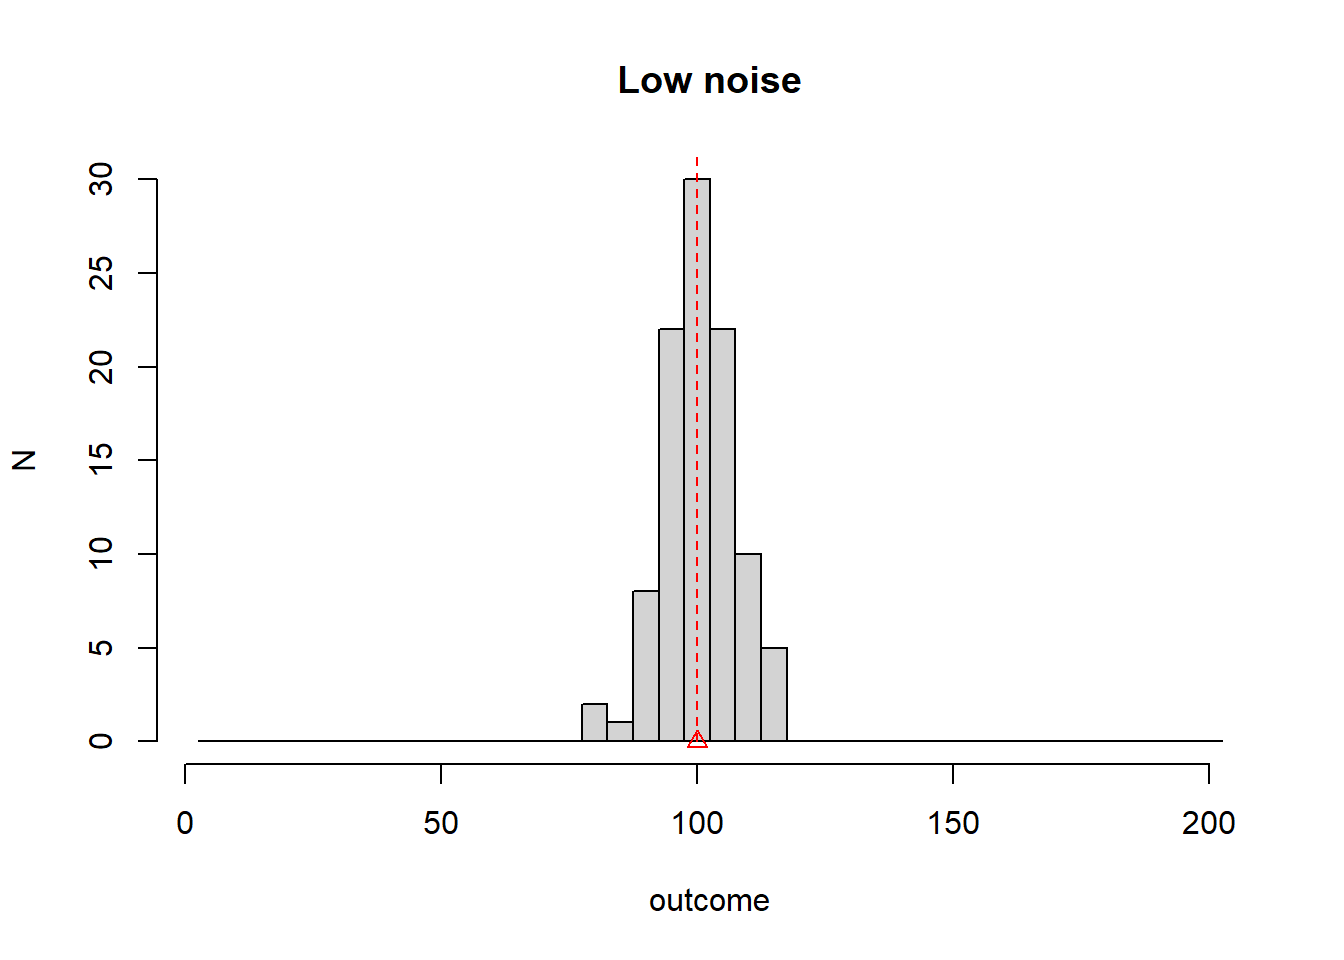
\includegraphics{_main_files/figure-latex/unnamed-chunk-23-1.pdf}

\hypertarget{diagrama-de-caja}{%
\section{Diagrama de caja}\label{diagrama-de-caja}}

El rango intercuartílico, la mediana y los \(5\%\) y \(95\%\) de los datos se pueden visualizar en un \textbf{diagrama de caja}.

En el diagrama de caja, los valores de los resultados están en el eje y. El IQR es la caja, la mediana es la línea del medio y los bigotes marcan los \(5\%\) y \(95\%\) de los datos.

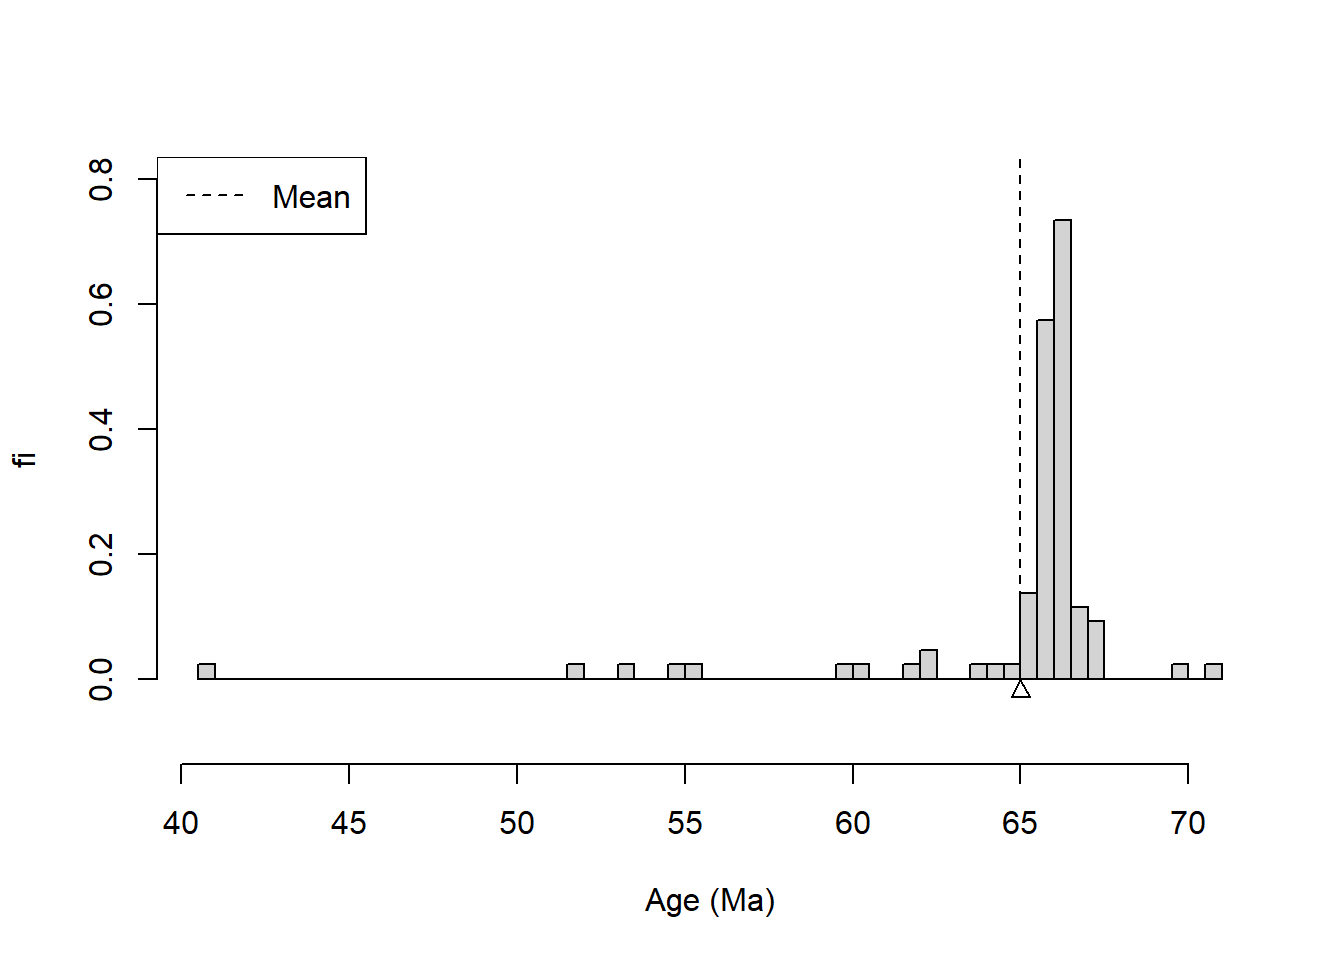
\includegraphics{_main_files/figure-latex/unnamed-chunk-24-1.pdf}

\hypertarget{preguntas}{%
\section{Preguntas}\label{preguntas}}

\textbf{1)} En el siguiente diagrama de caja, el primer cuartil y el segundo cuartil de los datos son:

\textbf{\(\qquad\)a:} \((-1.00, 21.30)\); \textbf{\(\qquad\)b:} \((-1.00, 7.02)\); \textbf{\(\qquad\)c:} \((7.02, 7.96)\); \textbf{\(\qquad\)d:} \((7.02, 14.22)\)

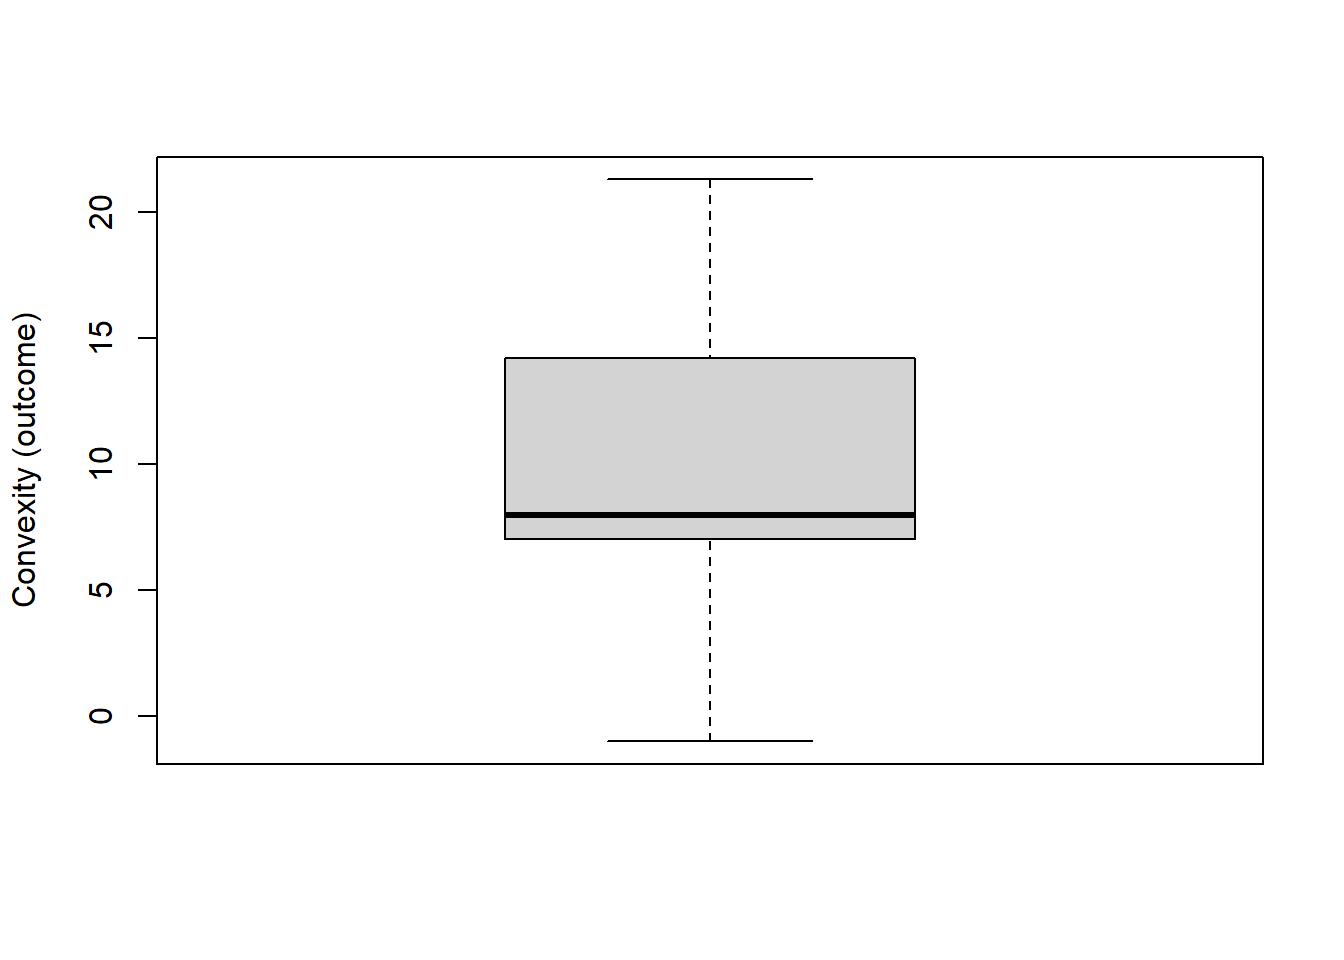
\includegraphics{./figures/box.png}

\textbf{2)} La principal desventaja de un histograma es que:

\textbf{\(\qquad\)a:} Depende del tamaño del bin; \textbf{\(\qquad\)b:} No se puede utilizar para variables categóricas;
\textbf{\(\qquad\)c:} No se puede usar cuando el tamaño del bin es pequeño;
\textbf{\(\qquad\)d:} Se usa solo para frecuencias relativas;

\textbf{3)} Si las frecuencias acumuladas relativas de un experimento aleatorio con resultados \(\{1,2,3,4\}\) son: \(F(1)=0.15, \qquad F(2)=0.60, \qquad F(3)=0.85, \qquad F(4)=1\).

Entonces la frecuencia relativa para el resultado \(3\) es

\textbf{\(\qquad\)a:} \(0.15\); \textbf{\(\qquad\)b:} \(0.85\); \textbf{\(\qquad\)c:} \(0.45\); \textbf{\(\qquad\)d:} \(0.25\)

\textbf{4)} En una muestra de tamaño \(10\) de un experimento aleatorio obtuvimos los siguientes datos:

\(8,\qquad 3,\qquad 3,\qquad 7,\qquad 3,\qquad 6,\qquad 5,\qquad 10,\qquad 3,\qquad 8\).

El primer cuartil de los datos es:

\textbf{\(\qquad\)a:} \(3.5\); \textbf{\(\qquad\)b:} \(4\); \textbf{\(\qquad\)c:} \(5\); \textbf{\(\qquad\)d:} \(3\)

\textbf{5)} Imaginemos que recopilamos datos para dos cantidades que no son mutuamente excluyentes, por ejemplo, el sexo y la nacionalidad de los pasajeros de un vuelo. Si queremos hacer un solo gráfico circular para los datos, ¿cuál de estas afirmaciones es verdadera?

\textbf{\(\qquad\)a:} Solo podemos hacer un gráfico circular de nacionalidad porque tiene más de dos resultados posibles; \textbf{\(\qquad\)b:} Podemos hacer un gráfico circular para una variable nueva que marca el sexo \textbf{y} la nacionalidad; \textbf{\(\qquad\)c:} Podemos hacer un gráfico circular para la variale sexo o la variable nacionalidad; \textbf{\(\qquad\)d:} Solo podemos elegir si hacemos un gráfico circular para el sexo o un gráfico circular para la nacionalidad.

\hypertarget{ejercicios}{%
\section{Ejercicios}\label{ejercicios}}

\hypertarget{ejercicio-1}{%
\subsubsection{Ejercicio 1}\label{ejercicio-1}}

Hemos realizado un experimento 8 veces con los siguientes resultados

\begin{verbatim}
## [1]  3  3 10  2  6 11  5  4
\end{verbatim}

Responde las siguientes cuestiones:

\begin{itemize}
\tightlist
\item
  Calcula las frecuencias relativas de cada resultado.
\item
  Calcula las frecuencias acumuladas de cada resultado.
\item
  ¿Cuál es el promedio de las observaciones?
\item
  ¿Cuál es la mediana?
\item
  ¿Cuál es el tercer cuartil?
\item
  ¿Cuál es el primer cuartil?
\end{itemize}

\hypertarget{ejercicio-2}{%
\subsubsection{Ejercicio 2}\label{ejercicio-2}}

Hemos realizado un experimento 10 veces con los siguientes resultados

\begin{verbatim}
##  [1] 2.875775 7.883051 4.089769 8.830174 9.404673 0.455565 5.281055 8.924190
##  [9] 5.514350 4.566147
\end{verbatim}

Considera 10 bins de tamaño 1: {[}0,1{]}, (1,2{]}\ldots(9,10).

Responde las siguientes cuestiones:

\begin{itemize}
\item
  Calcula las frecuencias relativas de cada resultado y dibuja el histograma
\item
  Calcula las frecuencias acumulativas de cada resultado y dibuja la gráfica acumulativa.
\item
  Dibuja un diagrama de caja .
\end{itemize}

\hypertarget{probabilidad}{%
\chapter{Probabilidad}\label{probabilidad}}

En este capítulo introduciremos el concepto de probabilidad a partir de frecuencias relativas.

Definiremos los eventos como los elementos sobre los que se aplica la probabilidad. Los eventos compuestos se definirán usando álgebra de conjuntos.

Luego discutiremos el concepto de probabilidad condicional derivado de la probabilidad conjunta de dos eventos.

\hypertarget{experimentos-aleatorios-1}{%
\section{Experimentos aleatorios}\label{experimentos-aleatorios-1}}

Recordemos el objetivo básico de la estadística. La estadística se ocupa de los datos que se presentan en forma de observaciones.

\begin{itemize}
\tightlist
\item
  Una \textbf{observación} es la adquisición de un número o una característica de un experimento
\end{itemize}

Las observaciones son realizaciones de \textbf{resultados}.

\begin{itemize}
\tightlist
\item
  Un \textbf{resultado} es una posible observación que es el resultado de un experimento.
\end{itemize}

Al realizar experimentos, a menudo obtenemos resultados diferentes. La descripción de la variabilidad de los resultados es uno de los objetivos de la estadística.

\begin{itemize}
\tightlist
\item
  Un \textbf{experimento aleatorio} es un experimento que da diferentes resultados cuando se repite de la misma manera.
\end{itemize}

La pregunta filosófica detrás es ¿Cómo podemos conocer algo si cada vez que lo miramos cambia?

\hypertarget{probabilidad-de-mediciuxf3n}{%
\section{Probabilidad de medición}\label{probabilidad-de-mediciuxf3n}}

Nos gustaría tener una medida para el resultado de un experimento aleatorio que nos diga \textbf{cuán seguros} estamos de observar el resultado cuando realicemos un \textbf{futuro} experimento aleatorio.

Llamaremos a esta medida la probabilidad del resultado y le asignaremos valores:

\begin{itemize}
\item
  0, cuando estamos seguros de que la observación \textbf{no} ocurrirá.
\item
  1, cuando estamos seguros de que la observación sucederá.
\end{itemize}

\hypertarget{probabilidad-cluxe1sica}{%
\section{Probabilidad clásica}\label{probabilidad-cluxe1sica}}

\textbf{Siempre que} un experimento aleatorio tenga \(M\) resultados posibles que son todos \textbf{igualmente probables}, la probabilidad de cada resultado \(i\) es \[P_i=\frac{1}{M}\].

La probabilidad clásica fue defendida por Laplace (1814).

Dado que cada resultado es \textbf{igualmente probable} en este tipo de experimento, declaramos una completa ignorancia y lo mejor que podemos hacer es distribuir equitativamente la misma probabilidad para cada resultado.

\begin{itemize}
\tightlist
\item
  No observamos \(P_i\)
\item
  Deducimos \(P_i\) de nuestra razón y no necesitamos realizar ningún experimento para conocerla.
\end{itemize}

\textbf{Ejemplo (dado):}

¿Cuál es la probabilidad de que obtengamos \(2\) en el lanzamiento de un dado?

\(P_2=1/6=0.166666\).

\hypertarget{frecuencias-relativas-1}{%
\section{Frecuencias relativas}\label{frecuencias-relativas-1}}

¿Qué sucede con los experimentos aleatorios cuyos posibles resultados \textbf{no} son igualmente probables?

¿Cómo podemos entonces definir las probabilidades de los resultados?

\textbf{Ejemplo (experimento aleatorio)}

Imaginemos que repetimos un experimento aleatorio \(8\) veces y obtenemos las siguientes observaciones

8 4 12 7 10 7 9 12

\begin{itemize}
\tightlist
\item
  ¿Qué tan seguro estamos de obtener el resultado \(12\) en la siguiente observación?
\end{itemize}

La tabla de frecuencias es

\begin{verbatim}
##   outcome ni    fi
## 1       4  1 0.125
## 2       7  2 0.250
## 3       8  1 0.125
## 4       9  1 0.125
## 5      10  1 0.125
## 6      12  2 0.250
\end{verbatim}

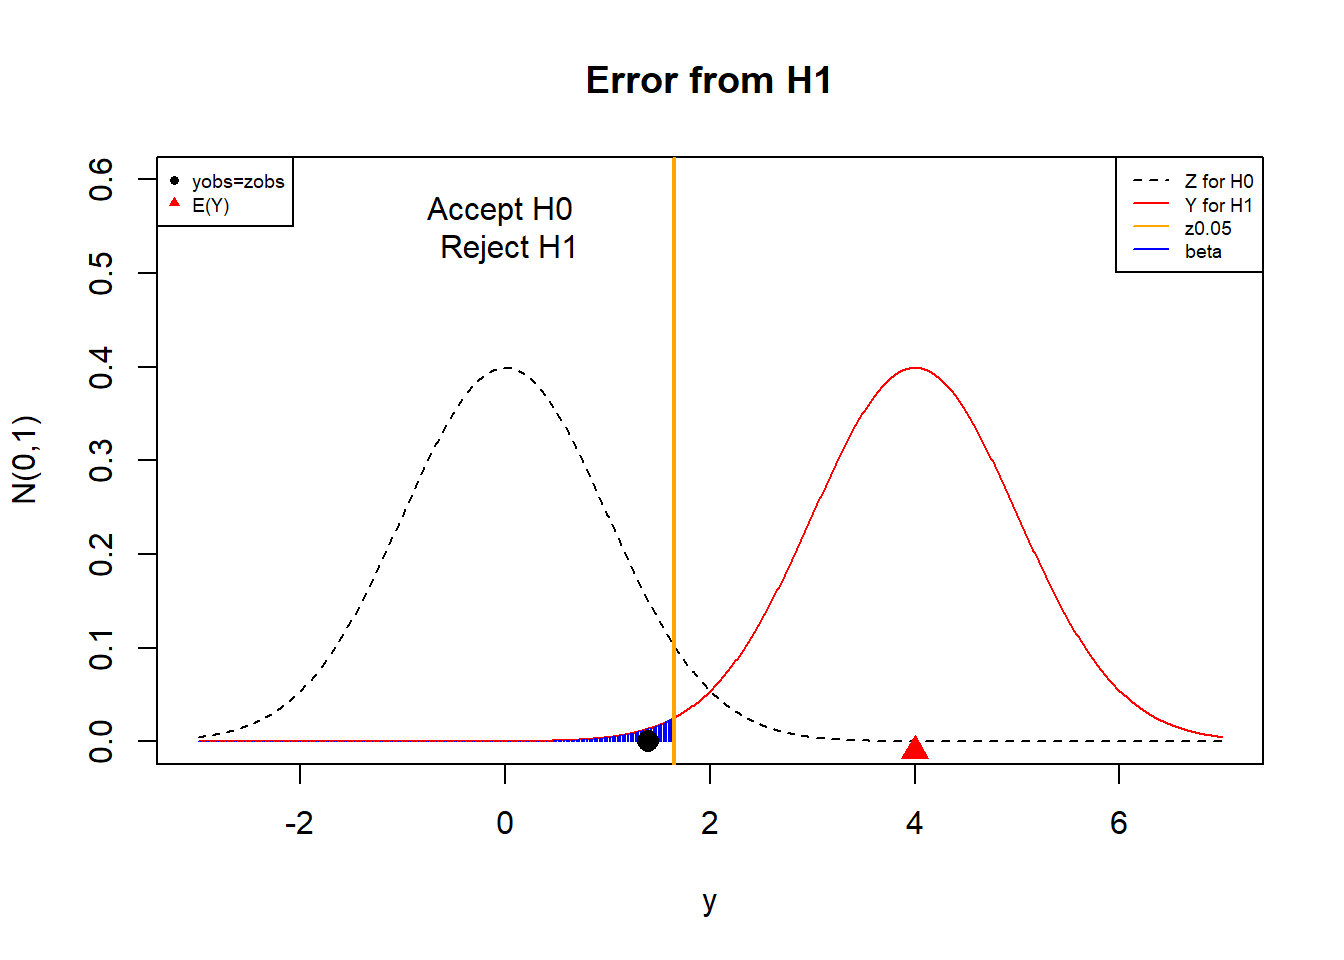
\includegraphics{_main_files/figure-latex/unnamed-chunk-28-1.pdf}
La \textbf{frecuencia relativa} \(f_i=\frac{n_i}{N}\) parece una medida de probabilidad razonable porque

\begin{itemize}
\tightlist
\item
  es un número entre \(0\) y \(1\).
\item
  mide la proporción del total de observaciones que observamos de un resultado particular.
\end{itemize}

Como \(f_{12}=0.25\) entonces estaríamos un cuarto seguros, una de cada 4 observaciones, de obtener \(12\).

\textbf{Pregunta}: ¿Qué tan bueno es \(f_i\) como medida de certeza del resultado \(i\)?

\textbf{Ejemplo (experimento aleatorio con mas repeticiones)}

Digamos que repetimos el experimento 100000 veces más:

La tabla de frecuencias es ahora

\begin{verbatim}
##    outcome    ni      fi
## 1        2  2807 0.02807
## 2        3  5607 0.05607
## 3        4  8435 0.08435
## 4        5 11070 0.11070
## 5        6 13940 0.13940
## 6        7 16613 0.16613
## 7        8 13806 0.13806
## 8        9 10962 0.10962
## 9       10  8402 0.08402
## 10      11  5581 0.05581
## 11      12  2777 0.02777
\end{verbatim}

y el gráfico de barras es

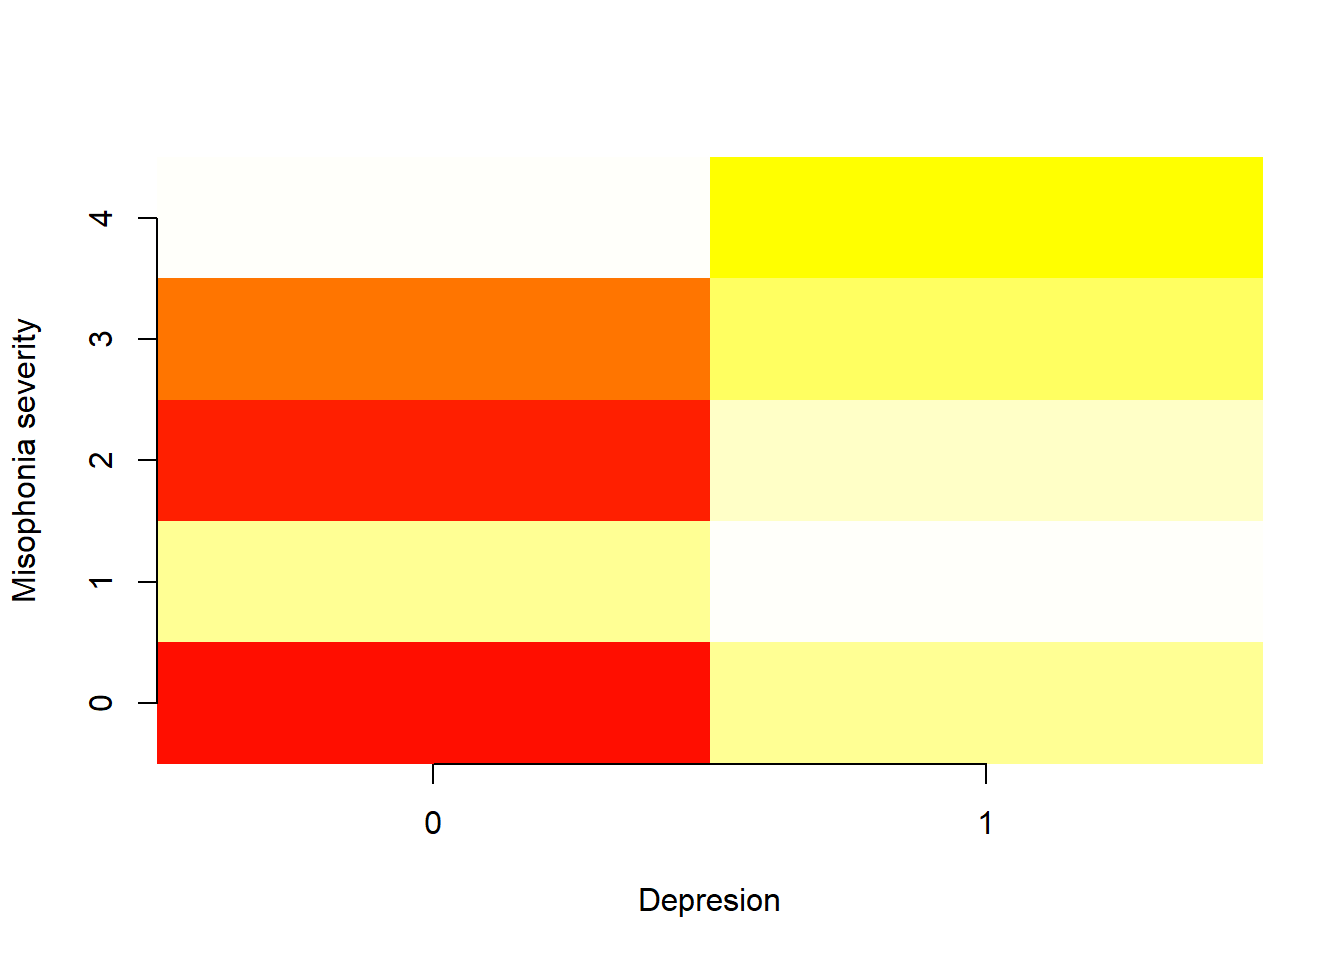
\includegraphics{_main_files/figure-latex/unnamed-chunk-30-1.pdf}

Aparecieron nuevos resultados y \(f_{12}\) ahora es solo \(0.027\), y entonces estamos sólo un \(\sim 3\%\) seguros de obtener \(12\) en el próximo experimento. Las probabilidades medidas por \(f_i\) cambian con \(N\).

\hypertarget{frecuencias-relativas-en-el-infinito}{%
\section{Frecuencias relativas en el infinito}\label{frecuencias-relativas-en-el-infinito}}

Una observación crucial es que si medimos las probabilidades de \(f_i\) en valores crecientes de \(N\) ¡\textbf{convergen}!

En este gráfico cada sección vertical da la frecuencia relativa de cada observación. Vemos que después de \(N=1000\) (\(log10(N)=3\)) las proporciones apenas varían con mas \(N\).

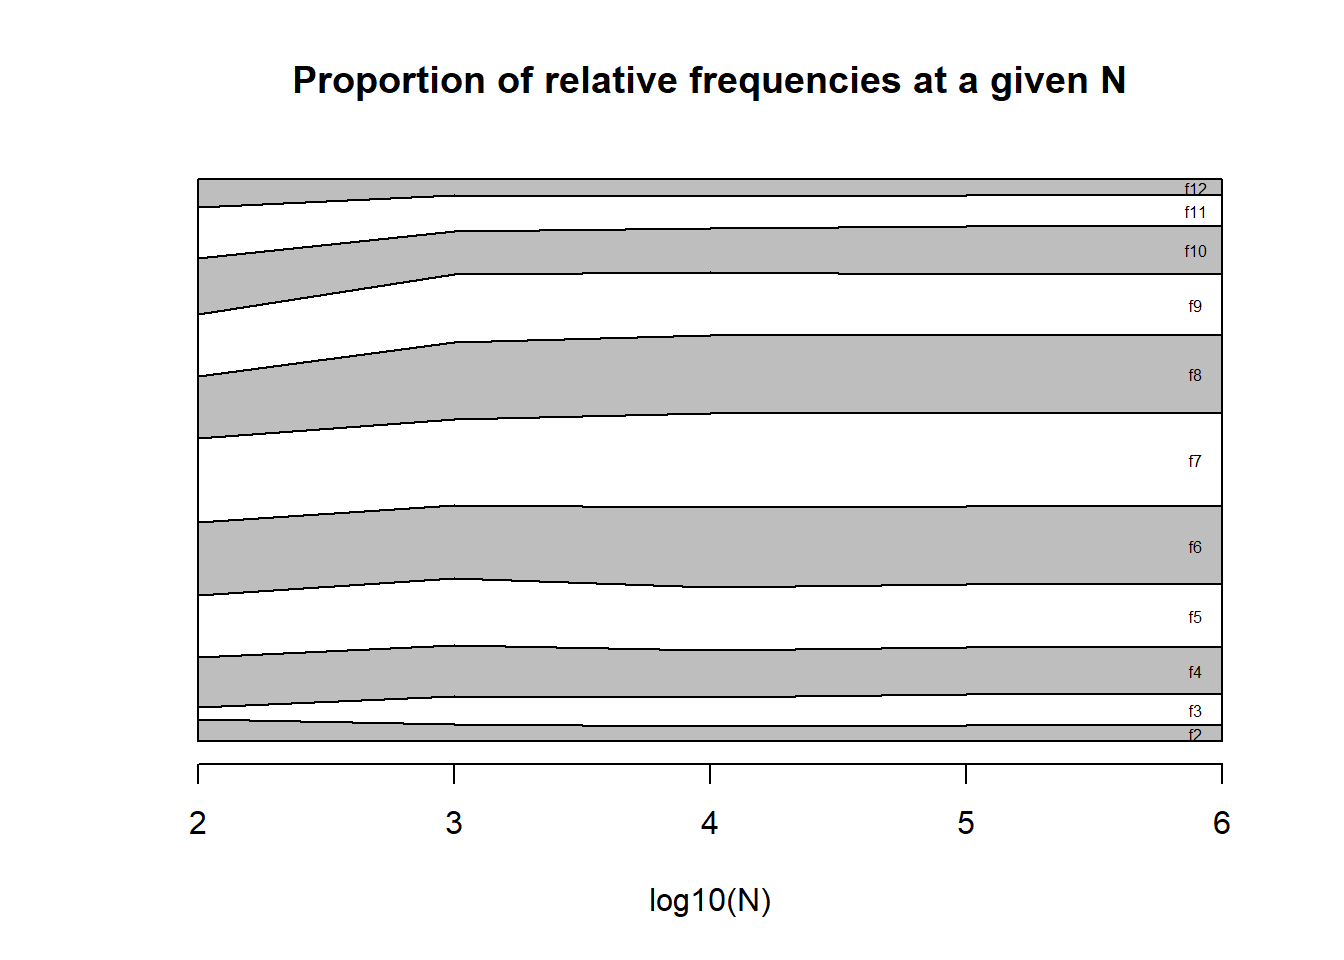
\includegraphics{_main_files/figure-latex/unnamed-chunk-31-1.pdf}
Encontramos que cada una de las frecuencias relativas \(f_i\) converge a un valor constante

\[lim_{N\rightarrow \infty} f_i = P_i\]

\hypertarget{probabilidad-frecuentista}{%
\section{Probabilidad frecuentista}\label{probabilidad-frecuentista}}

Llamamos \textbf{Probabilidad} \(P_i\) al límite cuando \(N \rightarrow \infty\) de la \textbf{frecuencia relativa} de observar el resultado \(i\) en un experimento aleatorio.

Defendida por Venn (1876), la definición frecuentista de probabilidad se deriva de datos/experiencia (empírica).

\begin{itemize}
\tightlist
\item
  No observamos \(P_i\), observamos \(f_i\)
\item
  \textbf{Estimamos} \(P_i\) con \(f_i\) (normalmente cuando \(N\) es grande), escribimos: \[\hat{P_i}=f_i\]
\end{itemize}

Similar a la relación entre \textbf{observación} y \textbf{resultado}, tenemos la relación entre \textbf{frecuencia relativa} y \textbf{probabilidad} como un valor concreto de una cantidad abstracta.

\hypertarget{probabilidades-cluxe1sicas-y-frecuentistas}{%
\section{Probabilidades clásicas y frecuentistas}\label{probabilidades-cluxe1sicas-y-frecuentistas}}

Tenemos situaciones en las que se puede usar la probabilidad clásica para encontrar el límite de frecuencias relativas.

\begin{itemize}
\tightlist
\item
  Si los resultados son \textbf{igualmente probables}, la probabilidad clásica nos da el límite:
\end{itemize}

\[P_i=lim_{N\rightarrow \infty} \frac{n_i}{N}=\frac{1}{M}\]

\begin{itemize}
\tightlist
\item
  Si los resultados en los que estamos interesados pueden derivarse de otros resultados \textbf{igualmente probables}; Veremos más sobre esto cuando estudiemos los modelos de probabilidad.
\end{itemize}

\textbf{Ejemplo (suma de dos dados)}

Nuestro ejemplo anterior se basa en la \textbf{suma de dos dados}.
Si bien realizamos el experimento muchas veces, anotamos los resultados y calculamos las \textbf{frecuencias relativas}, podemos conocer el valor exacto de probabilidad.

Esta probabilidad \textbf{se deduce} del hecho de que el resultado de cada dado es \textbf{igualmente probable}. A partir de esta suposición, podemos encontrar que (Ejercicio 1)

\[
    P_i= 
\begin{cases}
   \frac{i-1}{36},& i \in \{2,3,4,5,6, 7\} \\
\frac{13-i}{36},& i \in \{8,9,10,11,12\} \\ 
\end{cases}
\]

La motivación de la definición frecuentista es \textbf{empírica} (datos) mientras que la de la definición clásica es \textbf{racional} (modelos). A menudo combinamos ambos enfoques (inferencia y deducción) para conocer las probabilidades de nuestro experimento aleatorio.

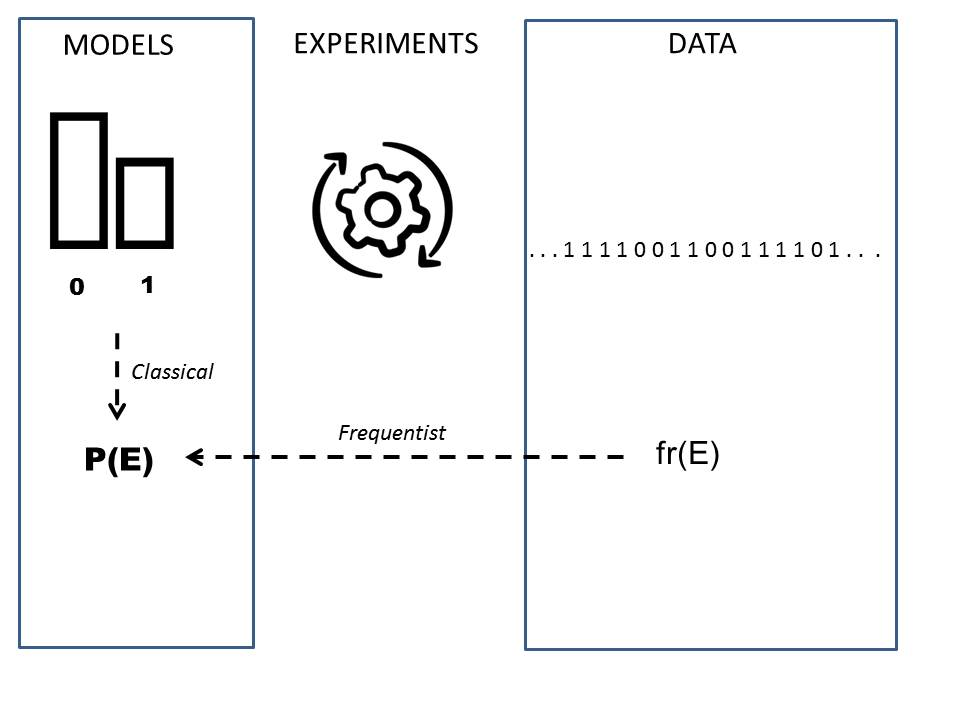
\includegraphics{./figures/prob.JPG}

\hypertarget{definiciuxf3n-de-probabilidad}{%
\section{Definición de probabilidad}\label{definiciuxf3n-de-probabilidad}}

Una probabilidad es un número que se asigna a cada resultado posible de un experimento aleatorio y satisface las siguientes propiedades o \textbf{axiomas}:

\begin{enumerate}
\def\labelenumi{\arabic{enumi})}
\tightlist
\item
  cuando los resultados \(E_1\) y \(E_2\) son mutuamente excluyentes; es decir, solo uno de ellos puede ocurrir, entonces la probabilidad de observar \(E_1\) \textbf{o} \(E_1\), escrito como \(E_1\cup E_2\), es su suma:
  \[P(E_1\cup E_2) = P(E_1) + P(E_2)\]
\item
  cuando \(S\) es el conjunto de todos los resultados posibles, entonces su probabilidad es \(1\) (al menos se observa algo): \[P(S)=1\]
\item
  La probabilidad de cualquier resultado está entre 0 y 1 \[P(E) \in [0,1]\]
\end{enumerate}

Propuesto por Kolmogorov's hace menos de 100 años (1933)

\hypertarget{tabla-de-probabilidades}{%
\section{Tabla de probabilidades}\label{tabla-de-probabilidades}}

Las propiedades de Kolmogorov son las reglas básicas para construir una \textbf{tabla de probabilidad}, de manera similar a la tabla de frecuencia relativa.

\textbf{Ejemplo (Dado)}

La tabla de probabilidad para el lanzamiento de un dado

\begin{longtable}[]{@{}cc@{}}
\toprule\noalign{}
resultado & Probabilidad \\
\midrule\noalign{}
\endhead
\bottomrule\noalign{}
\endlastfoot
\(1\) & 1/6 \\
\(2\) & 1/6 \\
\(3\) & 1/6 \\
\(4\) & 1/6 \\
\(5\) & 1/6 \\
\(6\) & 1/6 \\
\(P(1 \cup 2\cup ... \cup 6)\) & 1 \\
\end{longtable}

Verifiquemos los axiomas:

\begin{enumerate}
\def\labelenumi{\arabic{enumi})}
\item
  Donde \(1 \cup 2\) es, por ejemplo, el \textbf{evento} de lanzar un \(1\) \textbf{o} un \(2\). Entonces \[P(1 \cup 2)=P(1)+P(2)=2/6\]
\item
  Como \(S=\{1,2,3,4,5,6\}\) se compone de resultados \textbf{mutuamente excluyentes}, entonces
\end{enumerate}

\[P(S)=P(1\cup 2\cup ... \cup 6) = P(1)+P(2)+ ...+P(n)=1\]

\begin{enumerate}
\def\labelenumi{\arabic{enumi})}
\setcounter{enumi}{2}
\tightlist
\item
  Las probabilidades de cada uno de resultados están entre \(0\) y \(1\).
\end{enumerate}

\hypertarget{espacio-muestral}{%
\section{Espacio muestral}\label{espacio-muestral}}

El conjunto de todos los resultados posibles de un experimento aleatorio se denomina \textbf{espacio muestral} y se denota como \(S\).

El espacio muestral puede estar formado por resultados categóricos o numéricos.

\emph{Por ejemplo:}

\begin{itemize}
\tightlist
\item
  temperatura humana: \(S = (36, 42)\) grados Celsius.
\item
  niveles de azúcar en humanos: \(S=(70-80) mg/dL\)
\item
  el tamaño de un tornillo de una línea de producción: \(S=(70-72) mm\)
\item
  número de correos electrónicos recibidos en una hora: \(S =\{1, ...\infty \}\)
\item
  el lanzamiento de un dado: \(S=\{1, 2, 3, 4, 5, 6\}\)
\end{itemize}

\hypertarget{eventos}{%
\section{Eventos}\label{eventos}}

Un \textbf{evento} \(A\) es un \textbf{subconjunto} del espacio muestral. Es una \textbf{colección} de resultados.

\emph{Ejemplos de eventos:}

\begin{itemize}
\tightlist
\item
  El evento de una temperatura saludable: \(A=37-38\) grados Celsius
\item
  El evento de producir un tornillo con un tamaño: \(A=71.5mm\)
\item
  El evento de recibir más de 4 emails en una hora: \(A=\{4, \infty \}\)
\item
  El evento de obtener un número menor o igual a 3 en la tirada de a dice: \(A=\{1,2,3\}\)
\end{itemize}

Un evento se refiere a un posible conjunto de \textbf{resultados}.

\hypertarget{uxe1lgebra-de-eventos}{%
\section{Álgebra de eventos}\label{uxe1lgebra-de-eventos}}

Para dos eventos \(A\) y \(B\), podemos construir los siguientes eventos derivados utilizando las operaciones básicas de conjuntos:

\begin{itemize}
\tightlist
\item
  Complemento \(A'\): el evento de \textbf{no} \(A\)
\item
  Unión \(A \cup B\): el evento de \(A\) \textbf{o} \(B\)
\item
  Intersección \(A \cap B\): el evento de \(A\) \textbf{y} \(B\)
\end{itemize}

\textbf{Ejemplo (dado)}

Lancemos un dado y veamos los eventos (conjunto de resultados):

\begin{itemize}
\tightlist
\item
  un número menor o igual a tres \(A:\{1,2,3\}\)
\item
  un número par \(B:\{2,4,6\}\)
\end{itemize}

Veamos como podemos construir nuevos eventos con las operaciones de conjuntos:

\begin{itemize}
\tightlist
\item
  un número no menor de tres: \(A':\{4,5,6\}\)
\item
  un número menor o igual a tres \textbf{o} par: \(A \cup B: \{1,2,3,4,6\}\)
\item
  un número menor o igual a tres \textbf{y} par \(A \cap B: \{2\}\)
\end{itemize}

\hypertarget{resultados-mutuamente-excluyentes}{%
\section{Resultados mutuamente excluyentes}\label{resultados-mutuamente-excluyentes}}

Los resultados como tirar \(1\) y \(2\) en un dado son eventos que no pueden ocurrir al mismo tiempo. Decimos que son \textbf{mutuamente excluyentes}.

En general, dos eventos denotados como \(E_1\) y \(E_2\) son mutuamente excluyentes cuando

\[E_1\cap E_2=\emptyset\]

\emph{Ejemplos:}

\begin{itemize}
\item
  El resultado de tener una gravedad de misofonía de \(1\) y una gravedad de \(4\).
\item
  Los resultados de obtener \(12\) y \(5\) al sumar el lanzamiento de dos dados.
\end{itemize}

De acuerdo con las propiedades de Kolmogorov, solo los resultados \textbf{mutuamente excluyentes} se pueden organizar en \textbf{tablas de probabilidad}, como en las tablas de frecuencias relativas.

\hypertarget{probabilidades-conjuntas}{%
\section{Probabilidades conjuntas}\label{probabilidades-conjuntas}}

La \textbf{probabilidad conjunta} de \(A\) y \(B\) es la probabilidad de \(A\) y \(B\). Eso es \[P(A \cap B)\] o \(P(A,B)\).

Para escribir probabilidades conjuntas de eventos no mutuamente excluyentes (\(A \cap B \neq \emptyset\)) en una tabla de probabilidad, notamos que siempre podemos descomponer el espacio muestral en conjuntos \textbf{mutuamente excluyentes} que involucran las intersecciones:

\(S=\{A\cap B, A \cap B', A'\cap B, A'\cap B'\}\)

\textbf{Consideremos el diagrama de Ven} para el ejemplo donde \(A\) es el evento que corresponde a sacar número menor o igual que 3 y \(B\) corresponde a un número par:

Las \textbf{marginales} de \(A\) y \(B\) son la probabilidad de \(A\) y la probabilidad de \(B\), respectivamente:

\begin{itemize}
\tightlist
\item
  \(P(A)=P(A\cap B') + P(A \cap B)=2/6+1/6=3/6\)
\item
  \(P(B)=P(A'\cap B) +P(A \cap B)=2/6+1/6=3/6\)
\end{itemize}

Podemos ahora escribir la \textbf{tabla de probabilidad} para las probabilidades conjuntas

\begin{longtable}[]{@{}cc@{}}
\toprule\noalign{}
Resultado & Probabilidad \\
\midrule\noalign{}
\endhead
\bottomrule\noalign{}
\endlastfoot
\((A \cap B)\) & \(P(A \cap B)=1/6\) \\
\((A\cap B')\) & \(P(A \cap B')=2/6\) \\
\((A' \cap B)\) & \(P(A' \cap B)=2/6\) \\
\((A' \cap B')\) & \(P(A' \cap B')=1/6\) \\
suma & \(1\) \\
\end{longtable}

Cada resultado tiene \(dos\) valores (uno para la característica del tipo \(A\) y otro para el tipo \(B\))

\hypertarget{tabla-de-contingencia}{%
\section{Tabla de contingencia}\label{tabla-de-contingencia}}

La tabla de probabilidad conjunta también se puede escribir en una \textbf{tabla de contingencia}

\begin{longtable}[]{@{}cccc@{}}
\toprule\noalign{}
& \(B\) & \(B'\) & suma \\
\midrule\noalign{}
\endhead
\bottomrule\noalign{}
\endlastfoot
\(A\) & \(P(A \cap B )\) & \(P(A\cap B' )\) & \(P(A)\) \\
\(A'\) & \(P(A'\cap B )\) & \(P(A'\cap B' )\) & \(P(A')\) \\
suma & \(P(B)\) & \(P(B')\) & 1 \\
\end{longtable}

Donde las marginales son las sumas en las márgenes de la tabla, por ejemplo:

\begin{itemize}
\tightlist
\item
  \(P(A)=P(A \cap B') + P(A \cap B)\)
\item
  \(P(B)=P(A' \cap B) +P(A \cap B)\)
\end{itemize}

En nuestro ejemplo, la tabla de contingencia es

\begin{longtable}[]{@{}cccc@{}}
\toprule\noalign{}
& \(B\) & \(B'\) & suma \\
\midrule\noalign{}
\endhead
\bottomrule\noalign{}
\endlastfoot
\(A\) & \(1/6\) & \(2/6\) & \(3/6\) \\
\(A'\) & \(2/6\) & \(1/6\) & \(3/6\) \\
suma & \(3/6\) & \(3/6\) & 1 \\
\end{longtable}

\hypertarget{la-regla-de-la-suma}{%
\section{La regla de la suma:}\label{la-regla-de-la-suma}}

La regla de la suma nos permite calcular la probabilidad de \(A\) o \(B\), \(P(A \cup B)\), en términos de la probabilidad de \(A\) y \(B\), \(P(A \cap B)\). Podemos hacer esto de tres maneras equivalentes:

\begin{enumerate}
\def\labelenumi{\arabic{enumi})}
\item
  Usando las marginales y la probabilidad conjunta
  \[P(A \cup B)=P(A) + P(B) - P(A\cap B)\]
\item
  Usando solo probabilidades conjuntas
  \[P(A \cup B)=P(A \cap B)+P(A\cap B')+P(A'\cap B)\]
\item
  Usando el complemento de la probabilidad conjunta
  \[P(A \cup B)=1-P(A'\cap B')\]
\end{enumerate}

\textbf{Ejemplo (dado)}

Tomemos los eventos \(A:\{1,2,3\}\), sacar un número menor o igual que \(3\), y \(B:\{2,4,6\}\), sacar un número par en el lanzamiento de un dado.

Por lo tanto:

\begin{enumerate}
\def\labelenumi{\arabic{enumi})}
\item
  \(P(A \cup B)=P(A) + P(B) - P(A\cap B)=3/6+3/6-1/6=5/6\)
\item
  \(P(A \cup B)=P(A \cap B)+P(A\cap B')+P(A'\cap B)=1/6+2/6+2/6=5/6\)
\item
  \(P(A \cup B)=1-P(A'\cap B')= 1-1/6=5/6\)
\end{enumerate}

En la tabla de contingencia \(P(A \cup B)\) corresponde a las casillas en negrita (método 2 arriba), o todas menos el 1/6 de abajo a la derecha (método 3).

\begin{longtable}[]{@{}ccc@{}}
\toprule\noalign{}
& \(B\) & \(B'\) \\
\midrule\noalign{}
\endhead
\bottomrule\noalign{}
\endlastfoot
\(A\) & \textbf{1/6} & \textbf{2/6} \\
\(A'\) & \textbf{2/6} & \emph{1/6} \\
\end{longtable}

\hypertarget{preguntas-1}{%
\section{Preguntas}\label{preguntas-1}}

Recopilamos la edad y categoría de 100 deportistas en una competición

\begin{longtable}[]{@{}ccc@{}}
\toprule\noalign{}
& \(edad:junior\) & \(edad:senior\) \\
\midrule\noalign{}
\endhead
\bottomrule\noalign{}
\endlastfoot
\(categoria:1ra\) & \(14\) & \(12\) \\
\(categoria:2a\) & \(21\) & \(18\) \\
\(categoria:3a\) & \(22\) & \(13\) \\
\end{longtable}

\textbf{1)} ¿Cuál es la probabilidad estimada de que un deportista sea de 2ª categoría y senior?

\textbf{\(\qquad\)a:} \(18/100\); \textbf{\(\qquad\)b:} \(18/43\); \textbf{\(\qquad\)c:} \(18\); \textbf{\(\qquad\)d:} \(18/39\)

\textbf{2)} ¿Cuál es la probabilidad estimada de que el atleta no esté en la tercera categoría y sea senior?

\textbf{\(\qquad\)a:} \(35/100\); \textbf{\(\qquad\)b:} \(30/100\); \textbf{\(\qquad\)c:} \(22/100\); \textbf{\(\qquad\)d:} \(13/100\)

\textbf{3)} ¿Cuál es la probabilidad marginal de la tercera categoría?

\textbf{\(\qquad\)a:} \(13/100\); \textbf{\(\qquad\)b:} \(35/100\); \textbf{\(\qquad\)c:} \(22/100\); \textbf{\(\qquad\)d:} \(13/22\)

\textbf{4)} ¿Cuál es la probabilidad marginal de ser senior?

\textbf{\(\qquad\)a:} \(13/100\); \textbf{\(\qquad\)b:} \(43/100\); \textbf{\(\qquad\)c:} \(43/57\); \textbf{\(\qquad\)d:} \(57/100\)

\textbf{5)} ¿Cuál es la probabilidad de ser senior o de tercera categoría?

\textbf{\(\qquad\)a:} \(65/100\); \textbf{\(\qquad\)b:} \(86/100\); \textbf{\(\qquad\)c:} \(78/100\); \textbf{\(\qquad\)d:} \(13/100\)

\hypertarget{ejercicios-1}{%
\section{Ejercicios}\label{ejercicios-1}}

\hypertarget{probabilidad-cluxe1sica-ejercicio-1}{%
\subsubsection{Probabilidad clásica: Ejercicio 1}\label{probabilidad-cluxe1sica-ejercicio-1}}

\begin{itemize}
\item
  Escribe la tabla de \textbf{probabilidad conjunta} para los \textbf{resultados} de lanzar dos dados; en las filas escribe los resultados del primer dado y en las columnas los resultados del segundo dado.
\item
  ¿Cuál es la probabilidad de sacar \((3,4)\)? (R:1/36)
\item
  ¿Cuál es la probabilidad de tirar \(3\) y \(4\) con cualquiera de los dos dados? (R:2/36)
\item
  ¿Cuál es la probabilidad de tirar \(3\) en el primer dado o \(4\) en el segundo? (A:11/36)
\item
  ¿Cuál es la probabilidad de tirar \(3\) o \(4\) con cualquier dado? (R:20/36)
\item
  Escribe la \textbf{tabla de probabilidad} para el resultado de la \textbf{suma} de dos dados. Supon que el resultado de cada dado es \textbf{igualmente probable}. Verifica que es:
\end{itemize}

\[
    P_i= 
\begin{cases}
   \frac{i-1}{36},& i \in \{2,3,4,5,6, 7\} \\
\frac{13-i}{36},& i \in \{8,9,10,11,12\} \\ 
\end{cases}
\]

\hypertarget{probabilidad-frecuentista-ejercicio-2}{%
\subsubsection{Probabilidad frecuentista: Ejercicio 2}\label{probabilidad-frecuentista-ejercicio-2}}

El resultado de un experimento aleatorio es medir la gravedad de la misofonía \textbf{y} el estado de depresión de un paciente.

\begin{itemize}
\tightlist
\item
  Gravedad de la misofonía: \(S_M:\{M_0,M_1,M_2,M_3,M_4\}\)
\item
  Depresión: \(S_D:\{D', D\}\))
\end{itemize}

Escribe la tabla de contingencia para las frecuencias absolutas (\(n_{M,D}\)) para un estudio sobre un total de 123 pacientes en el que se observó

\begin{itemize}
\tightlist
\item
  100 individuos no tuvieron depresión.
\item
  Ningún individuo con misofonía 4 y sin depresión.
\item
  5 individuos con misofonía de grado 1 y sin depresión.
\item
  El mismo número que el caso anterior para individuos con depresión y sin misofonía.
\item
  25 individuos sin depresión y grado 3 de misofonía.
\item
  El número de misofónicos sin depresión para los grados 2 y 0 se repartieron a cantiaddes iguales.
\item
  El número de individuos con depresión y misofonía incrementó progresivamente
  en múltiplos de tres, empezando en 0 individuos para grado 1.
\end{itemize}

Reponde las siguientes preguntas:

\begin{itemize}
\tightlist
\item
  ¿Cuantos individuos tuvieron misofonía? (R:83)
\item
  ¿Cuantos individuos tuvieron misofonía de grado 3? (R:31)
\item
  ¿Cuantos individuos tuvieron misofonía de grado 2 sin depresión? (R:35)
\end{itemize}

Escribe las tabla de consingencia para frecuencias relativas \(f_{M,D}\). Supongamos que \(N\) es grande y que las frecuencias absolutas \textbf{estiman} las probabilidades \(f_{M,D}=\hat{P}(M \cap D)\). Responde las siguientes preguntas:

\begin{itemize}
\tightlist
\item
  ¿Cuál es la probabilidad marginal de misofonía de gravedad 2? (R: 0.3)
\item
  ¿Cuál es la probabilidad de no ser misofónico \textbf{y} no estar deprimido? (R:0.284)
\item
  ¿Cuál es la probabilidad de ser misofónico \textbf{o} estar deprimido? (R: 0.715)
\item
  ¿Cuál es la probabilidad de ser misofónico \textbf{y} estar deprimido? (R: 0.146)
\item
  Describir en lenguaje hablado los resultados con probabilidad 0.
\end{itemize}

\hypertarget{ejercicio-3}{%
\subsubsection{Ejercicio 3}\label{ejercicio-3}}

Hemos realizado un experimento aleatorio \(10\) veces, que consiste en anotar el sexo y el estado vital de pacientes con algún tipo de cáncer después de 10 años del diagnóstico. Obtuvimos los siguientes resultados

\begin{verbatim}
##         A     B
## 1    male  dead
## 2    male  dead
## 3    male  dead
## 4  female alive
## 5    male  dead
## 6  female alive
## 7  female  dead
## 8  female alive
## 9    male alive
## 10   male alive
\end{verbatim}

\begin{itemize}
\tightlist
\item
  Crea la tabla de contingencia para el número (\(n_{i,j}\)) de observaciones de cada resultado (\(A,B\))
\item
  Crea la tabla de contingencia para la frecuencia relativa (\(f_{i,j}\)) de los resultados
\item
  ¿Cuál es la frecuencia marginal de ser hombre? (R/0.6)
\item
  ¿Cuál es la frecuencia marginal de estar vivo? (R/0.5)
\item
  ¿Cuál es la frecuencia de estar vivo \textbf{o} ser mujer? (R/0.6)
\end{itemize}

\hypertarget{teoruxeda-ejercicio-4}{%
\subsubsection{Teoría: Ejercicio 4}\label{teoruxeda-ejercicio-4}}

\begin{itemize}
\item
  De la segunda forma de la regla de la suma, obtener la primera y la tercera forma.
\item
  ¿Cuál es la regla de la suma de la tercera forma para la probabilidad de tres eventos \(P(A \cup B \cup C)\)?
\end{itemize}

\hypertarget{probabilidad-condicional}{%
\chapter{Probabilidad condicional}\label{probabilidad-condicional}}

En este capítulo, introduciremos la probabilidad condicional.

Usaremos la probabilidad condicional para definir la independencia estadística.

Discutiremos el teorema de Bayes y discutiremos una de sus principales aplicaciones, que es la eficacia de predicción de una herramienta de diagnóstico.

\hypertarget{probabilidad-conjunta}{%
\section{Probabilidad conjunta}\label{probabilidad-conjunta}}

Recordemos que la probabilidad conjunta de dos eventos \(A\) y \(B\) se define como su intersección

\[P( A,B )=P(A \cap B)\]

Ahora, imagina experimentos aleatorios que miden dos tipos diferentes de resultados.

\begin{itemize}
\item
  altura y peso de un individuo: \((h, w)\)
\item
  tiempo y posición de una carga eléctrica: \((p, t)\)
\item
  el lanzamiento de dos dados: (\(n_1\),\(n_2\))
\item
  cruzar dos semáforos en verde: (\(\bar{R_ 1}\) , \(\bar{R_2}\))
\end{itemize}

A menudo nos interesa saber si los valores de un resultado \textbf{condicionan} los valores del otro.

\hypertarget{independencia-estaduxedstica}{%
\section{Independencia estadística}\label{independencia-estaduxedstica}}

En muchos casos, estamos interesados en saber si dos eventos a menudo tienden a ocurrir juntos. Queremos poder discernir entre dos casos.

\begin{itemize}
\item
  \textbf{Independencia} entre eventos. Por ejemplo, sacar un 1 en un dado no hace más probable sacar otro 1 en un segundo dado.
\item
  \textbf{Correlación} entre eventos. Por ejemplo, si un hombre es alto, probablemente sea pesado.
\end{itemize}

\textbf{Ejemplo (conductor)}

Realizamos un experimento para averiguar si observar fallas estructurales en un material afecta su conductividad.

Los datos se verían como

\begin{longtable}[]{@{}ccc@{}}
\toprule\noalign{}
Conductor & Estructura & Conductividad \\
\midrule\noalign{}
\endhead
\bottomrule\noalign{}
\endlastfoot
\(c_1\) & con fallas & defectuosa \\
\(c_2\) & sin fallas & sin defectos \\
\(c_3\) & con fallas & defectuosa \\
\ldots{} & \ldots{} & \ldots{} \\
\(c_i\) & sin fallas & defectuosa* \\
\ldots{} & \ldots{} & \ldots{} \\
\ldots{} & \ldots{} & \ldots{} \\
\(c_n\) & con fallas & sin defectos* \\
\end{longtable}

Podemos esperar que la conductividad defectuosa ocurra más a menudo con fallas que sin fallas si las fallas afectan la conductividad.

Imaginemos que a partir de los datos obtenemos la siguiente tabla de contingencia de \textbf{probabilidades conjuntas} estimadas

\begin{longtable}[]{@{}cccc@{}}
\toprule\noalign{}
& con fallas (F) & sin fallas (F') & suma \\
\midrule\noalign{}
\endhead
\bottomrule\noalign{}
\endlastfoot
defectuoso (D) & \(0.005\) & \(0.045\) & \(0.05\) \\
sin defectos (D') & \(0.095\) & \(0.855\) & \(0.95\) \\
suma & \(0.1\) & \(0.9\) & 1 \\
\end{longtable}

donde, por ejemplo, la probabilidad conjunta de \(F\) y \(D\) es

\begin{itemize}
\tightlist
\item
  \(P(D,F)=0.005\)
\end{itemize}

y las probabilidades marginales son

\begin{itemize}
\tightlist
\item
  \(P(D)=P(D, F) + P(D, F')=0.05\)
\item
  \(P(F)=P(D, F) + P(D', F)= 0.1\).
\end{itemize}

\hypertarget{la-probabilidad-condicional}{%
\section{La probabilidad condicional}\label{la-probabilidad-condicional}}

La conductividad defectuosa es \textbf{independiente} de tener fallas estructurales en el material si la probabilidad de tener conductividad defectuosa (\(D\)) es la misma \textbf{ya sea} que tenga fallas (\(F\)) o no (\(F'\)) .

Consideremos primero solamente los materiales que tienen fallas.

Dentro de aquellos materiales que tienen fallas (\(F\)), ¿cuál es la probabilidad estimada de que sean defectuosos?

\(\hat{P}(D|F)=\frac{n_{F,D}}{n_{F}}=\frac{n_{F,D}/n}{n_{F}/n}= \frac{f_{F,D}}{f_{F}}\)
\[= \frac{\hat{P}(F,D)}{\hat{P}(F)}\]
Por lo tanto, en el límite cuando \(N \rightarrow \infty\), tenemos

\[P(D|F)=\frac{P(F, D)}{P(D)}=\frac{P(F \cap D)}{P(D)}\]
\textbf{Definición:}

La \emph{probabilidad condicional} de un evento \(B\) dado un evento \(A\), indicado como \(P(A|B)\), es
\[P(A|B) = \frac{P(A\cap B)}{P(B)}\]
Podemos probar que la probabilidad condicional satisface los axiomas de probabilidad. La probabilidad condicional se puede entender como una probabilidad con un espacio muestral dado por \(B\): \(S_B\). En nuestro ejemplo, los materiales con fallas.

\hypertarget{tabla-de-contingencia-condicional}{%
\section{Tabla de contingencia condicional}\label{tabla-de-contingencia-condicional}}

Si dividimos las columnas de la tabla de probabilidad conjunta por las probabilidades marginales de los efectos condicionantes (\(F\) y \(F'\)), podemos escribir \textbf{una tabla de contingencia condicional}

\begin{longtable}[]{@{}
  >{\centering\arraybackslash}p{(\columnwidth - 4\tabcolsep) * \real{0.3438}}
  >{\centering\arraybackslash}p{(\columnwidth - 4\tabcolsep) * \real{0.3438}}
  >{\centering\arraybackslash}p{(\columnwidth - 4\tabcolsep) * \real{0.3125}}@{}}
\toprule\noalign{}
\begin{minipage}[b]{\linewidth}\centering
\end{minipage} & \begin{minipage}[b]{\linewidth}\centering
F
\end{minipage} & \begin{minipage}[b]{\linewidth}\centering
F'
\end{minipage} \\
\midrule\noalign{}
\endhead
\bottomrule\noalign{}
\endlastfoot
D & P(D {\textbar{}} F) & P(D {\textbar{}} F') \\
D' & P(D' {\textbar{}} F) & P(D' {\textbar{}} F') \\
suma & 1 & 1 \\
\end{longtable}

Donde las probabilidades por columnas suman uno. La primera columna muestra las probabilidades de ser defectuoso o no solo de que los materiales que tienen fallas (primera condición: \(F\)). La segunda columna muestra las probabilidades solo para los materiales que no tienen fallas (segunda condición: \(F'\)).

Las probabilidades condicionales son las probabilidades del evento dentro de cada condición. Las leemos como:

\begin{itemize}
\item
  \(P(D|F)\): Probabilidad de tener conductividad defectuosa \textbf{si} tiene fallas
\item
  \(P(D'|F)\): Probabilidad de no tener conductividad defectuosa \textbf{si} tiene fallas
\item
  \(P(D|F')\): Probabilidad de tener conductividad defectuosa \textbf{si} no tiene fallas
\item
  \(P(D'|F')\) Probabilidad de no tener conductividad defectuosa \textbf{si} no tiene fallas
\end{itemize}

\hypertarget{independencia-estaduxedstica-1}{%
\section{Independencia estadística}\label{independencia-estaduxedstica-1}}

En nuestro ejemplo, la tabla de contingencia condicional es

\begin{longtable}[]{@{}
  >{\centering\arraybackslash}p{(\columnwidth - 4\tabcolsep) * \real{0.3438}}
  >{\centering\arraybackslash}p{(\columnwidth - 4\tabcolsep) * \real{0.3438}}
  >{\centering\arraybackslash}p{(\columnwidth - 4\tabcolsep) * \real{0.3125}}@{}}
\toprule\noalign{}
\begin{minipage}[b]{\linewidth}\centering
\end{minipage} & \begin{minipage}[b]{\linewidth}\centering
F
\end{minipage} & \begin{minipage}[b]{\linewidth}\centering
F'
\end{minipage} \\
\midrule\noalign{}
\endhead
\bottomrule\noalign{}
\endlastfoot
D & P(D{\textbar{}}F) = 0.05 & P(D{\textbar{}}F')=0.05 \\
D' & P(D'{\textbar{}}F)=0.95 & P(D'{\textbar{}}F')=0.95 \\
suma & 1 & 1 \\
\end{longtable}

¡Observamos que las probabilidades marginales y condicionales son las mismas!

\begin{itemize}
\tightlist
\item
  \(P(D|F)=P(D|F')=P(D)\)
\item
  \(P(D'|F)=P(D'|F')=P(D')\)
\end{itemize}

Esto quiere decir que la probabilidad de observar un conductor defectuoso \textbf{no} depende tener una falla estructural o no.

Concluimos que la conductividad defectuosa no se ve afectada por tener una falla estructural.

\textbf{Definición}

Dos eventos \(A\) y \(B\) son estadísticamente independientes si ocurre cualquiera de los casos equivalentes

\begin{enumerate}
\def\labelenumi{\arabic{enumi})}
\tightlist
\item
  \(P(A|B)=P(A)\); \(A\) es independiente de \(B\)
\item
  \(P(B|A)=P(B)\); \(B\) es independiente de \(A\)
\end{enumerate}

y por la definición de probabilidad condicional

\begin{enumerate}
\def\labelenumi{\arabic{enumi})}
\setcounter{enumi}{2}
\tightlist
\item
  \(P(A\cap B)=P(A|B)P(B)=P(A)P(B)\)
\end{enumerate}

Esta tercera forma es un enunciado sobre las probabilidades conjuntas. Dice que podemos obtener probabilidades conjuntas por la multiplicación de las marginales.

En nuestra tabla de probabilidad conjunta original

\begin{longtable}[]{@{}cccc@{}}
\toprule\noalign{}
& F & F' & suma \\
\midrule\noalign{}
\endhead
\bottomrule\noalign{}
\endlastfoot
D & \(0.005\) & \(0.045\) & \(0.05\) \\
D' & \(0.095\) & \(0.855\) & \(0.95\) \\
suma & \(0.1\) & \(0.9\) & 1 \\
\end{longtable}

podemos confirmar que todas las entradas de la matriz son el producto de las marginales. Por ejemplo: \(P(F)P(D)= P(D \cap F)\) y \(P(D')P(F')=P(D' \cap F')\). Por lo tanto, ser defectuoso es independiente de tener un defecto.

\textbf{Ejemplo (Monedas)}

Queremos confirmar que los resultados de lanzar dos monedas son independientes. Consideramos que todos los resultados son igualmente probables:

\begin{longtable}[]{@{}cc@{}}
\toprule\noalign{}
resultado & Probabilidad \\
\midrule\noalign{}
\endhead
\bottomrule\noalign{}
\endlastfoot
\((H,T)\) & 1/4 \\
\((H,H)\) & 1/4 \\
\((T,T)\) & 1/4 \\
\((T,H)\) & 1/4 \\
suma & 1 \\
\end{longtable}

donde \((H,T)\) es, por ejemplo, el evento de cara en la primera moneda y cruz en la segunda moneda. La tabla de contingencia para las probabilidades conjuntas es:

\begin{longtable}[]{@{}cccc@{}}
\toprule\noalign{}
& H & T & suma \\
\midrule\noalign{}
\endhead
\bottomrule\noalign{}
\endlastfoot
H & \(1/4\) & \(1/4\) & \(1/2\) \\
T & \(1/4\) & \(1/4\) & \(1/2\) \\
suma & \(1/2\) & \(1/2\) & 1 \\
\end{longtable}

De esta tabla vemos que la probabilidad de obtener una cara y luego una cruz es el producto de las marginales \(P(H, T)=P(H)*P(T)=1/4\). Por lo tanto, el evento de cara en la primera moneda y cruz en la segunda son independientes.

Si elaboramos la tabla de contingencia condicional sobre el lanzamiento de la primera moneda veremos que obtener cruz en la segunda moneda no está condicionado por haber obtenido cara en la primera moneda: \(P(T|H)=P(T) =1/2\)

\hypertarget{dependencia-estaduxedstica}{%
\section{Dependencia estadística}\label{dependencia-estaduxedstica}}

Un ejemplo importante de dependencia estadística se encuentra en el desempeño de \textbf{herramientas de diagnóstico}, donde queremos determinar el estado de un sistema (s) con resultados

\begin{itemize}
\tightlist
\item
  inadecuado (si)
\item
  adecuado (no)
\end{itemize}

con una prueba (t) con resultados

\begin{itemize}
\tightlist
\item
  positivo
\item
  negativo
\end{itemize}

Por ejemplo, probamos una batería para saber cuánto tiempo puede durar. Tensamos un cable para saber si resiste llevar cierta carga. Realizamos una PCR para ver si alguien está infectado.

\hypertarget{prueba-de-diagnuxf3stico}{%
\section{Prueba de diagnóstico}\label{prueba-de-diagnuxf3stico}}

Consideremos diagnosticar una infección con una nueva prueba. Estado de infección:

\begin{itemize}
\tightlist
\item
  si (infectado)
\item
  no (no infectado)
\end{itemize}

Prueba:

\begin{itemize}
\tightlist
\item
  positivo
\item
  negativo
\end{itemize}

La \textbf{tabla de contingencia condicional} es lo que obtenemos en un ambiente controlado (laboratorio)

\begin{longtable}[]{@{}
  >{\centering\arraybackslash}p{(\columnwidth - 4\tabcolsep) * \real{0.3438}}
  >{\centering\arraybackslash}p{(\columnwidth - 4\tabcolsep) * \real{0.3438}}
  >{\centering\arraybackslash}p{(\columnwidth - 4\tabcolsep) * \real{0.3125}}@{}}
\toprule\noalign{}
\begin{minipage}[b]{\linewidth}\centering
\end{minipage} & \begin{minipage}[b]{\linewidth}\centering
Infección: si
\end{minipage} & \begin{minipage}[b]{\linewidth}\centering
Infección: No
\end{minipage} \\
\midrule\noalign{}
\endhead
\bottomrule\noalign{}
\endlastfoot
Test: positivo & P(positivo {\textbar{}} si) & P(positivo {\textbar{}} no) \\
Test: negativo & P(negativo {\textbar{}} si) & P(negativo {\textbar{}} no) \\
suma & 1 & 1 \\
\end{longtable}

Miremos las entradas de la tabla
1) Tasa de verdaderos positivos (Sensibilidad): La probabilidad de dar positivo \textbf{si} tiene la enfermedad \(P(positivo|si)\)

\begin{enumerate}
\def\labelenumi{\arabic{enumi})}
\setcounter{enumi}{1}
\item
  Tasa de verdaderos negativos (Especificidad): La probabilidad de dar negativo \textbf{si} no tiene la enfermedad \(P(negativo|no)\)
\item
  Tasa de falsos positivos: la probabilidad de dar positivo \textbf{si} no tiene la enfermedad \(P(positivo|no)\)
\item
  Tasa de falsos negativos: la probabilidad de dar negativo \textbf{si} tiene la enfermedad \(P(negativo|si)\)
\end{enumerate}

Alta correlación (dependencia estadística) entre la prueba y la infección significa valores altos de las probabilidades 1 y 2 \textbf{y} valores bajos para las probabilidades 3 y 4.

\textbf{Ejemplo (COVID)}

Ahora consideremos una situación real. En los días iniciales de la pandemia de coronavirus no había una medida de la eficacia de las PCR para detectar el virus. Uno de los primeros estudios publicados (\url{https://www.nejm.org/doi/full/10.1056/NEJMp2015897}) encontró que

\begin{itemize}
\tightlist
\item
  Las PCR tuvieron una sensibilidad del 70\%, en condición de infección.
\item
  Las PCR tuvieron una especificidad del 94\%, en condición de no infección.
\end{itemize}

La tabla de contingencia condicional es

\begin{longtable}[]{@{}
  >{\centering\arraybackslash}p{(\columnwidth - 4\tabcolsep) * \real{0.3438}}
  >{\centering\arraybackslash}p{(\columnwidth - 4\tabcolsep) * \real{0.3438}}
  >{\centering\arraybackslash}p{(\columnwidth - 4\tabcolsep) * \real{0.3125}}@{}}
\toprule\noalign{}
\begin{minipage}[b]{\linewidth}\centering
\end{minipage} & \begin{minipage}[b]{\linewidth}\centering
Infección: si
\end{minipage} & \begin{minipage}[b]{\linewidth}\centering
Infección: No
\end{minipage} \\
\midrule\noalign{}
\endhead
\bottomrule\noalign{}
\endlastfoot
Test: positivo & P(positivo{\textbar{}}si)=0.7 & P(positivo{\textbar{}}no)=0.06 \\
Test: negativo & P(negativo{\textbar{}}si)=0.3 & P(negativo{\textbar{}}no)=0.94 \\
suma & 1 & 1 \\
\end{longtable}

Por lo tanto, los errores en las pruebas de diagnóstico fueron:

\begin{itemize}
\tightlist
\item
  La tasa de falsos positivos es \(P(positivo|no)=0.06\)
\item
  La tasa de falsos negativos es \(P(negativo|si)=0.3\)
\end{itemize}

\hypertarget{probabilidades-inversas}{%
\section{Probabilidades inversas}\label{probabilidades-inversas}}

Nos interesa encontrar la probabilidad de estar infectado si la prueba da positivo: \[P(si|positivo)\]

Para eso:

\begin{enumerate}
\def\labelenumi{\arabic{enumi}.}
\tightlist
\item
  Recuperamos la tabla de contingencia para probabilidades conjuntas, multiplicando por las marginales
\end{enumerate}

\begin{longtable}[]{@{}
  >{\centering\arraybackslash}p{(\columnwidth - 6\tabcolsep) * \real{0.2619}}
  >{\centering\arraybackslash}p{(\columnwidth - 6\tabcolsep) * \real{0.2619}}
  >{\centering\arraybackslash}p{(\columnwidth - 6\tabcolsep) * \real{0.2381}}
  >{\centering\arraybackslash}p{(\columnwidth - 6\tabcolsep) * \real{0.2381}}@{}}
\toprule\noalign{}
\begin{minipage}[b]{\linewidth}\centering
\end{minipage} & \begin{minipage}[b]{\linewidth}\centering
Infección: si
\end{minipage} & \begin{minipage}[b]{\linewidth}\centering
Infección: No
\end{minipage} & \begin{minipage}[b]{\linewidth}\centering
suma
\end{minipage} \\
\midrule\noalign{}
\endhead
\bottomrule\noalign{}
\endlastfoot
Test: positivo & P(positivo {\textbar{}} si)P(si) & P(positivo {\textbar{}} no)P(no) & P(positivo) \\
Test: negativo & P(negativo {\textbar{}} si)P(si) & P(negativo {\textbar{}} no) P(no) & P(negativo) \\
suma & P(si) & P(no) & 1 \\
\end{longtable}

\begin{enumerate}
\def\labelenumi{\arabic{enumi}.}
\setcounter{enumi}{1}
\tightlist
\item
  Usamos la definición de probabilidades condicionales para filas en lugar de columnas (dividimos por la marginal de los resultados de la prueba)
\end{enumerate}

\begin{longtable}[]{@{}
  >{\centering\arraybackslash}p{(\columnwidth - 6\tabcolsep) * \real{0.2619}}
  >{\centering\arraybackslash}p{(\columnwidth - 6\tabcolsep) * \real{0.2619}}
  >{\centering\arraybackslash}p{(\columnwidth - 6\tabcolsep) * \real{0.2381}}
  >{\centering\arraybackslash}p{(\columnwidth - 6\tabcolsep) * \real{0.2381}}@{}}
\toprule\noalign{}
\begin{minipage}[b]{\linewidth}\centering
\end{minipage} & \begin{minipage}[b]{\linewidth}\centering
Infección: si
\end{minipage} & \begin{minipage}[b]{\linewidth}\centering
Infección: No
\end{minipage} & \begin{minipage}[b]{\linewidth}\centering
suma
\end{minipage} \\
\midrule\noalign{}
\endhead
\bottomrule\noalign{}
\endlastfoot
Test: positivo & P(si{\textbar{}}positivo) & P(sin{\textbar{}}positivo) & 1 \\
Test: negativo & P(si{\textbar{}}negativo) & P(sin{\textbar{}}negativo) & 1 \\
\end{longtable}

Por ejemplo:

\[P(si|positivo)=\frac{P(positivo|si)P(si)}{P(positivo)}\]

Para aplicar esta fórmula necesitamos las marginales \(P(si)\) (incidencia) y \(P(positivo)\).

\begin{itemize}
\item
  Para encontrar \(P(si)\), necesitamos un nuevo estudio: el primer estudio de prevalencia en España mostró que durante el confinamiento \(P(si)=0.05\), \(P(no)=0.95\), antes del verano de 2020.
\item
  Para encontrar \(P(positivo)\), podemos usar la definición de probabilidad marginal y condicional:
\end{itemize}

\(P(positivo)=P(positivo \cap si) + P(positivo \cap no)\)
\[= P(positivo|si)P(si)+P(positivo|no)P(no)\]
Esta última relación de las marginales se llama \textbf{regla de probabilidad total}.

\hypertarget{teorema-de-bayes}{%
\section{Teorema de Bayes}\label{teorema-de-bayes}}

Después de sustituir la regla de probabilidad total en \(P(si|positivo)\), tenemos

\[P(si|positivo)=\frac{P(positivo|si)P(si)}{P(positivo|si)P(si)+P(positivo|no)P(no)}\]
Esta expresión se conoce como \textbf{teorema de Bayes}. Nos permite invertir los condicionales:

\[P(positivo|si) \rightarrow P(si|positivo)\]
O \textbf{evaluar} una prueba en una condición controlada (infección) y luego usarla para \textbf{inferir} la probabilidad de la condición cuando la prueba es positiva.

\textbf{Ejemplo (COVID)}:

El rendimiento de la prueba fue:

\begin{itemize}
\item
  Sensibilidad: \(P(positivo|si)=0.70\)
\item
  Tasa de falsos positivos: \(P(positivo|no)=1- P(negativo|no)=0.06\)
\end{itemize}

El estudio en población española dio:

\begin{itemize}
\tightlist
\item
  \(P(si)=0.05\)
\item
  \(P(no)=1-P(si)=0.95\).
\end{itemize}

Por lo tanto, la probabilidad de estar infectado en caso de dar positivo era:

\[P(si|positivo)=0.38\]

Concluimos que en ese momento las PCR no eran muy buenas para \textbf{confirmar} infecciones.

Sin embargo, apliquemos ahora el teorema de Bayes a la probabilidad de no estar infectado si la prueba fue negativa.

\[P(no|negativo) = \frac{P(negativo|no) P(no)}{P(negativo|no) P(no)+P(negativo|si)P(si)}\]

La sustitución de todos los valores da

\[P(no|negativo)=0.98\]

Por lo tanto, las pruebas eran buenas para \textbf{descartar} infecciones y un requisito justo para viajar.

\textbf{Teorema de Bayes}

En general, podemos tener más de dos eventos condicionantes. Por lo tanto, el teorema de Baye dice:

Si \(E1, E2, ..., Ek\) son \(k\) eventos mutuamente excluyentes y exhaustivos y \(B\) es cualquier evento, entonces la probabilidad inversa \(P(Ei|B)\) es

\[P(Ei|B)=\frac{P(B|Ei)P(Ei)}{P(B|E1)P(E1) +...+ P(B|Ek)P(Ek)} \]
El denominador es la regla de probabilidad total para la marginal \(P(B)\), en términos de las marginales \(P(E1), P(E2), ... P(Ek)\).

\[P(B)=P(B|E1)P(E1) +...+ P(B|Ek)P(Ek)\]

\textbf{Árbol condicional}

La regla de probabilidad total también se puede ilustrar usando un árbol \textbf{condicional}.

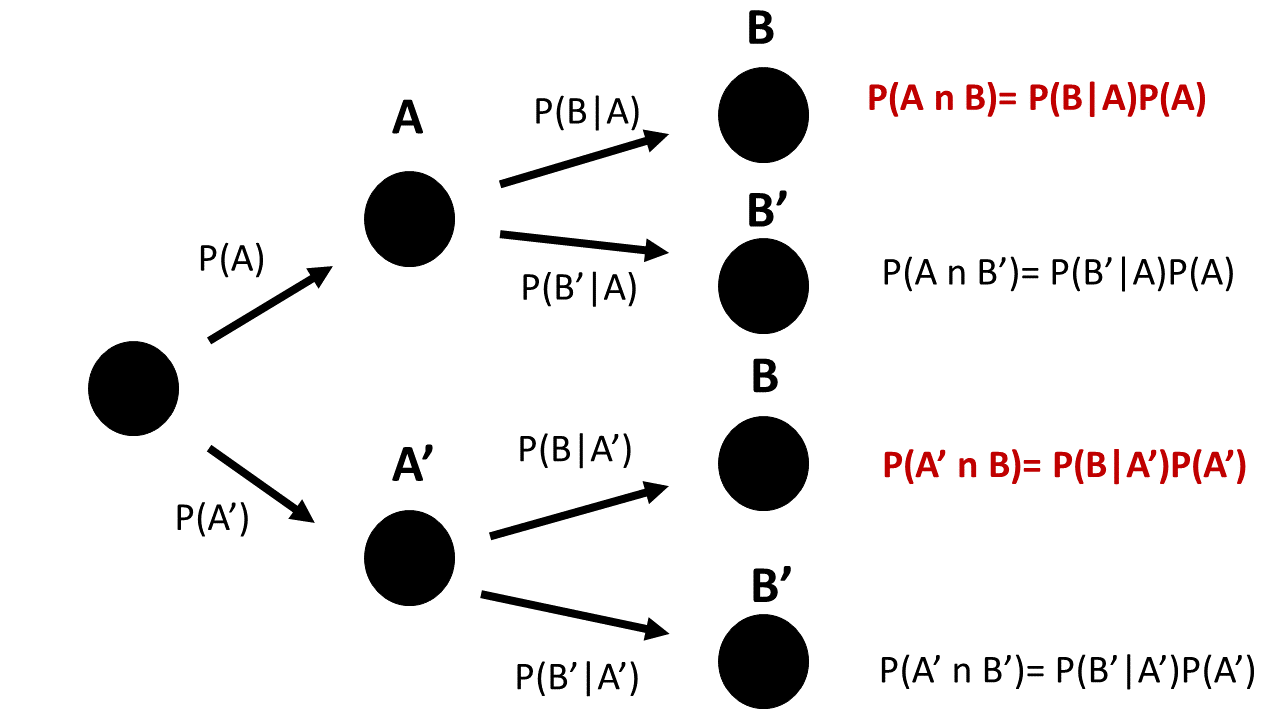
\includegraphics{./figures/treetot.PNG}

\textbf{Regla de probabilidad total} para la marginal de \(B\): ¿De cuántas maneras puedo obtener el resultado \(B\)?

\(P(B)=P(B|A)P(A)+P(B|A')P(A')\)

\hypertarget{preguntas-2}{%
\section{Preguntas}\label{preguntas-2}}

Recopilamos la edad y categoría de 100 deportistas en una competición

\begin{longtable}[]{@{}ccc@{}}
\toprule\noalign{}
& \(junior\) & \(senior\) \\
\midrule\noalign{}
\endhead
\bottomrule\noalign{}
\endlastfoot
\(1er\) & \(14\) & \(12\) \\
\(2do\) & \(21\) & \(18\) \\
\(3er\) & \(22\) & \(13\) \\
\end{longtable}

\textbf{1)} ¿Cuál es la probabilidad estimada de que el atleta esté en la tercera categoría si el atleta es junior?

\textbf{\(\qquad\)a:} \(22\); \textbf{\(\qquad\)b:} \(22/100\); \textbf{\(\qquad\)c:} \(22/57\); \textbf{\(\qquad\)d:} \(22/35\);

\textbf{2)} ¿Cuál es la probabilidad estimada de que el atleta sea junior y esté en 1ra categoría si el atleta no está en 3ra categoría?

\textbf{\(\qquad\)a:} \(14/35\); \textbf{\(\qquad\)b:} \(14/65\); \textbf{\(\qquad\)c:} \(14/100\); \textbf{\(\qquad\)d:} \(14/26\)

\textbf{3)} Una prueba diagnóstica tiene una probabilidad de \(8/9\) de detectar una enfermedad si los pacientes están enfermos y una probabilidad de \(3/9\) de detectar la enfermedad si los pacientes están sanos. Si la probabilidad de estar enfermo es \(1/9\). ¿Cuál es la probabilidad de que un paciente esté enfermo si una prueba detecta la enfermedad?

\textbf{\(\qquad\)a:} \(\frac{8/9}{8/9+3/9}*1/9\); \textbf{\(\qquad\)b:} \(\frac{3/9}{8/9+3/9}*1/9\); \textbf{\(\qquad\)c:} \(\frac{3/9*8/9}{8/9*1/9+3/9*8/9}\); \textbf{\(\qquad\)d:} \(\frac{8/9*1/9}{8/9*1/9+3/9*8/9}\);

\textbf{4)} Como se comenta en las notas, una prueba PCR para coronavirus tenía una sensibilidad del 70 \% y una especificidad del 94 \% y en España durante el confinamiento hubo una incidencia del 5 \%. Con estos datos, ¿cuál era la probabilidad de dar positivo en España (\(P(positivo)\))

\textbf{\(\qquad\)a:} \(0.035\); \textbf{\(\qquad\)b:} \(0.092\); \textbf{\(\qquad\)c:} \(0.908\); \textbf{\(\qquad\)d:} \(0.95\)

\textbf{5)} Con los mismos datos que en la pregunta 4, dar positivo en la PCR y estar infectado no son eventos independientes porque:

\textbf{\(\qquad\)a:} La sensibilidad es del 70\%; \textbf{\(\qquad\)b:} La sensibilidad y la tasa de falsos positivos son diferentes; \textbf{\(\qquad\)c:} La tasa de falsos positivos es del 0.06\%; \textbf{\(\qquad\)d:} la especificidad es del 96\%

\hypertarget{ejercicios-2}{%
\section{Ejercicios}\label{ejercicios-2}}

\hypertarget{ejercicio-1-1}{%
\subsubsection{Ejercicio 1}\label{ejercicio-1-1}}

Se prueba el rendimiento de una máquina para producir varillas de torneado de alta calidad. Estos son los resultados de las pruebas

\begin{longtable}[]{@{}ccc@{}}
\toprule\noalign{}
& Redondeado: si & Redondeado: No \\
\midrule\noalign{}
\endhead
\bottomrule\noalign{}
\endlastfoot
superficie lisa: si & 200 & 1 \\
superficie lisa: no & 4 & 2 \\
\end{longtable}

\begin{itemize}
\item
  ¿Cuál es la probabilidad estimada de que la máquina produzca una varilla que no satisfaga ningún control de calidad? (R: 2/207)
\item
  ¿Cuál es la probabilidad estimada de que la máquina produzca una varilla que no satisfaga al menos un control de calidad? (R: 7/207)
\item
  ¿Cuál es la probabilidad estimada de que la máquina produzca varillas de superficie redondeada y alisada? (R: 200/207)
\item
  ¿Cuál es la probabilidad estimada de que la barra sea redondeada si la barra es lisa? (R: 200/201)
\item
  ¿Cuál es la probabilidad estimada de que la varilla sea lisa si es redondeada? (R: 200/204)
\item
  ¿Cuál es la probabilidad estimada de que la varilla no sea ni lisa ni redondeada si no satisface al menos un control de calidad? (R: 2/7)
\item
  ¿Son eventos independientes la lisa y la redondez? (No)
\end{itemize}

\hypertarget{ejercicio-2-1}{%
\subsubsection{Ejercicio 2}\label{ejercicio-2-1}}

Desarrollamos un test para detectar la presencia de bacterias en un lago. Encontramos que si el lago contiene la bacteria, la prueba es positiva el 70\% de las veces. Si no hay bacterias, la prueba es negativa el 60\% de las veces. Implementamos la prueba en una región donde sabemos que el 20\% de los lagos tienen bacterias.

\begin{itemize}
\tightlist
\item
  ¿Cuál es la probabilidad de que un lago que dé positivo esté contaminado con bacterias? (R: 0.30)
\end{itemize}

\hypertarget{ejercicio-3-1}{%
\subsubsection{Ejercicio 3}\label{ejercicio-3-1}}

Se prueba el rendimiento de dos máquinas para producir varillas de torneado de alta calidad. Estos son los resultados de las pruebas

\textbf{Máquina 1}

\begin{longtable}[]{@{}ccc@{}}
\toprule\noalign{}
& Redondeado: si & Redondeado: No \\
\midrule\noalign{}
\endhead
\bottomrule\noalign{}
\endlastfoot
superficie lisa: si & 200 & 1 \\
superficie lisa: no & 4 & 2 \\
\end{longtable}

\textbf{Máquina 2}

\begin{longtable}[]{@{}ccc@{}}
\toprule\noalign{}
& Redondeado: si & Redondeado: No \\
\midrule\noalign{}
\endhead
\bottomrule\noalign{}
\endlastfoot
superficie lisa: si & 145 & 4 \\
superficie lisa: no & 8 & 6 \\
\end{longtable}

\begin{itemize}
\tightlist
\item
  ¿Cuál es la probabilidad de que la barra sea redondeada? (R: 357/370)
\item
  ¿Cuál es la probabilidad de que la varilla haya sido producida por la máquina 1? (R: 207/370)
\item
  ¿Cuál es la probabilidad de que la varilla no sea lisa? (R: 20/370)
\item
  ¿Cuál es la probabilidad de que la varilla sea lisa o redondeada o producida por la máquina 1? (R: 364/370)
\item
  ¿Cuál es la probabilidad de que la varilla quede redondeada si es alisada y de la máquina 1? (R: 200/201)
\item
  ¿Cuál es la probabilidad de que la varilla no esté redondeada si no está alisada y es de la máquina 2? (R: 6/14)
\item
  ¿Cuál es la probabilidad de que la varilla haya salido de la máquina 1 si está alisada y redondeada? (R: 200/345)
\item
  ¿Cuál es la probabilidad de que la varilla haya venido de la máquina 2 si no pasa al menos uno de los controles de calidad? (R:0.72)
\end{itemize}

\hypertarget{ejercicio-4}{%
\subsubsection{Ejercicio 4}\label{ejercicio-4}}

Queremos cruzar una avenida con dos semáforos. La probabilidad de encontrar el primer semáforo en rojo es 0.6. Si paramos en el primer semáforo, la probabilidad de parar en el segundo es 0.15. Mientras que la probabilidad de detenernos en el segundo si no nos detenemos en el primero es 0.25.

Cuando intentamos cruzar ambos semáforos:

\begin{itemize}
\tightlist
\item
  ¿Cuál es la probabilidad de tener que detenerse en cada semáforo? (R:0.09)
\item
  ¿Cuál es la probabilidad de tener que parar en al menos un semáforo? (R:0.7)
\item
  ¿Cuál es la probabilidad de tener que detenerse en un solo semáforo? (R:0.61)
\item
  Si paré en el segundo semáforo, ¿cuál es la probabilidad de que tuviera que parar en el primero? (R: 0.47)
\item
  Si tuviera que parar en cualquier semáforo, ¿cuál es la probabilidad de que tuviera que hacerlo dos veces? (R: 0.12)
\item
  ¿Parar en el primer semáforo es un evento independiente de detenerse en el segundo semáforo? (No)
\end{itemize}

Ahora, deseamos cruzar una avenida con tres semáforos. La probabilidad de encontrarnos con el primer semáforo en rojo es del 0.6, y la probabilidad de encontrar el segundo semáforo en rojo depende únicamente de la probabilidad del primer semáforo. De manera similar, la probabilidad de encontrar un semáforo en rojo en el tercer semáforo depende solo de las probabilidades del segundo. Como antes, la probabilidad de detenernos en un semáforo es del 0.15 si nos detuvimos en el semáforo anterior. Si no nos detuvimos en el semáforo anterior, la probabilidad de detenernos en el siguiente semáforo es del 0.25.

\begin{itemize}
\tightlist
\item
  ¿Cuál es la probabilidad de tener que parar en cada semáforo? (R:0.013)
\item
  ¿Cuál es la probabilidad de tener que parar en al menos un semáforo? (R:0.775)
\item
  ¿Cuál es la probabilidad de tener que detenerse en un solo semáforo? (R:0.5425)
\end{itemize}

consejos:

\begin{itemize}
\item
  Si la probabilidad de que un semáforo esté en rojo depende únicamente del anterior, entonces
  \(P(R_3|R_2,R_1)=P(R_3|R_2,\bar{R}_1)=P(R_3|R_2)\) y \(P(R_3|\bar{R}_2,R_1)=P(R_3 |\bar{R}_2,\bar{R}_1)=P(R_3|\bar{R}_2)\)
\item
  La probabilidad conjunta de encontrar tres semáforos en rojo se puede escribir como:
  \(P(R_1,R_2,R_3)=P(R_3|R_2)P(R_2|R_1)P(R_1)\)
\end{itemize}

\hypertarget{ejercicio-5}{%
\subsubsection{Ejercicio 5}\label{ejercicio-5}}

Una prueba de calidad en un ladrillo aleatorio se define por los eventos:

\begin{itemize}
\tightlist
\item
  Pasar la prueba de calidad: \(E\), no pasar la prueba de calidad: \(\bar{E}\)
\item
  Defectuoso: \(D\), no defectuoso: \(\bar{D}\)
\end{itemize}

Si la prueba diagnóstica tiene sensibilidad \(P(E|\bar{D})=0.99\) y especificidad \(P(\bar{E}|D)=0.98\), y la probabilidad de pasar la prueba es \(P(E) =0.893\) entonces

\begin{itemize}
\item
  ¿Cuál es la probabilidad de que un ladrillo elegido al azar sea defectuoso \(P(D)\)? (R:0.1)
\item
  ¿Cuál es la probabilidad de que un ladrillo que ha pasado la prueba sea realmente defectuoso? (R:0.022)
\item
  La probabilidad de que un ladrillo no sea defectuoso \textbf{y} que no pase la prueba (R:0.009)
\item
  ¿Son \(D\) y \(\bar{E}\) estadísticamente independientes? (No)
\end{itemize}

\hypertarget{variables-aleatorias-discretas}{%
\chapter{Variables aleatorias discretas}\label{variables-aleatorias-discretas}}

\hypertarget{objetivo-1}{%
\section{Objetivo}\label{objetivo-1}}

En este capítulo definiremos las variables aleatorias y estudiaremos variables aleatorias \textbf{discretas}.

Definiremos la función de masa de probabilidad y sus principales propiedades de media y varianza. Siguiendo el proceso de abstracción de las frecuencias relativas en probabilidades, también definimos la distribución de probabilidad como el caso límite de la frecuencia relativa acumulada.

\hypertarget{frecuencias-relativas-2}{%
\section{Frecuencias relativas}\label{frecuencias-relativas-2}}

Las frecuencias relativas de los resultados de un experimento aleatorio son una medida de su propensión. Podemos usarlos como estimadores de sus probabilidades, cuando repetimos el experimento aleatorio muchas veces (\(n \rightarrow \infty\)).

Definimos tendencia central (promedio), dispersión (varianza muestral) y la distribución de frecuencias de los datos (\(F_i\)).

En términos de probabilidades, ¿cómo se definen estas cantidades?

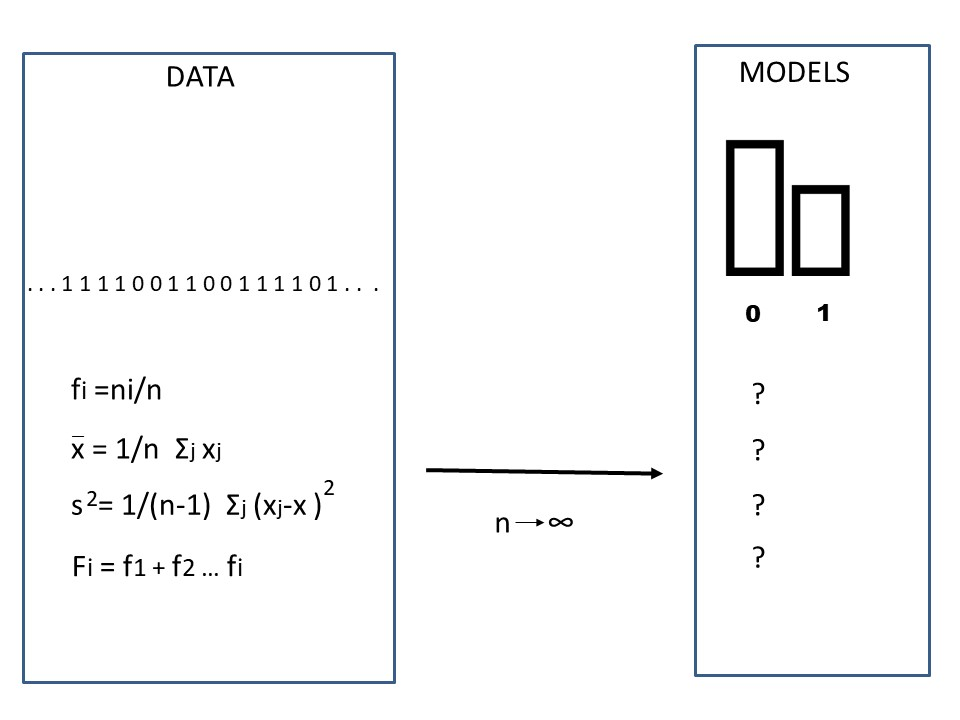
\includegraphics{./figures/randomvar.JPG}

\hypertarget{variable-aleatoria}{%
\section{Variable aleatoria}\label{variable-aleatoria}}

Definimos las frecuencias relativas sobre las \textbf{observaciones} de los experimentos. Ahora definimos las cantidades equivalentes para las probabilidades en términos de los \textbf{resultados} de los experimentos. Nos ocuparemos únicamente de resultados de tipo numérico.

Una \textbf{variable aleatoria} es un símbolo que representa un \textbf{resultado numérico} de un experimento aleatorio. Escribimos la variable aleatoria en \textbf{mayúsculas} (es decir, \(X\)).

\textbf{Definición:}

Una \textbf{variable aleatoria} es una función que asigna un \textbf{número} real a un \textbf{evento} del espacio muestral de un experimento aleatorio.

Recuerda que un evento puede ser un resultado o una colección de resultados.

Cuando la variable aleatoria toma un \textbf{valor}, indica la realización de un \textbf{evento} de un experimento aleatorio.

\emph{Ejemplo:}

Si \(X \in \{0,1\}\), entonces decimos que \(X\) es una variable aleatoria que puede tomar los valores \(0\) o \(1\).

\hypertarget{eventos-de-observar-una-variable-aleatoria}{%
\section{Eventos de observar una variable aleatoria}\label{eventos-de-observar-una-variable-aleatoria}}

Hacemos la distinción entre variables en el espacio modelo con letras mayúsculas, como entidades abstractas, y la realización de un evento o resultado particular. Por ejemplo:

\begin{itemize}
\tightlist
\item
  \(X=1\) es el \textbf{evento} de observar la variable aleatoria \(X\) con valor \(1\)
\item
  \(X=2\) es el \textbf{evento} de observar la variable aleatoria \(X\) con valor \(2\)
\end{itemize}

\ldots{}

\textbf{En general:}

\begin{itemize}
\tightlist
\item
  \(X=x\) es el \textbf{evento} de observar la variable aleatoria \(X\) (\(X\) mayúscula) con valor \(x\) (\(x\) pequeño).
\end{itemize}

\hypertarget{probabilidad-de-variables-aleatorias}{%
\section{Probabilidad de variables aleatorias}\label{probabilidad-de-variables-aleatorias}}

Nos interesa asignar probabilidades a los eventos de observar un valor particular de una variable aleatoria.

Por ejemplo, para los dados escribiremos la tabla de probabilidad como

\begin{longtable}[]{@{}cc@{}}
\toprule\noalign{}
\(X\) & Probabilidad \\
\midrule\noalign{}
\endhead
\bottomrule\noalign{}
\endlastfoot
\(1\) & \(P(X=1)=1/6\) \\
\(2\) & \(P(X=2)=1/6\) \\
\(3\) & \(P(X=3)=1/6\) \\
\(4\) & \(P(X=4)=1/6\) \\
\(5\) & \(P(X=5)=1/6\) \\
\(6\) & \(P(X=6)=1/6\) \\
\end{longtable}

donde hacemos explícitos los eventos de que la variable toma un resultado dado \(X=x\).

\hypertarget{funciones-de-probabilidad}{%
\section{Funciones de probabilidad}\label{funciones-de-probabilidad}}

Debido a que \(x\) (minúscula) es una variable numérica, las probabilidades de la variable aleatoria se pueden dibujar

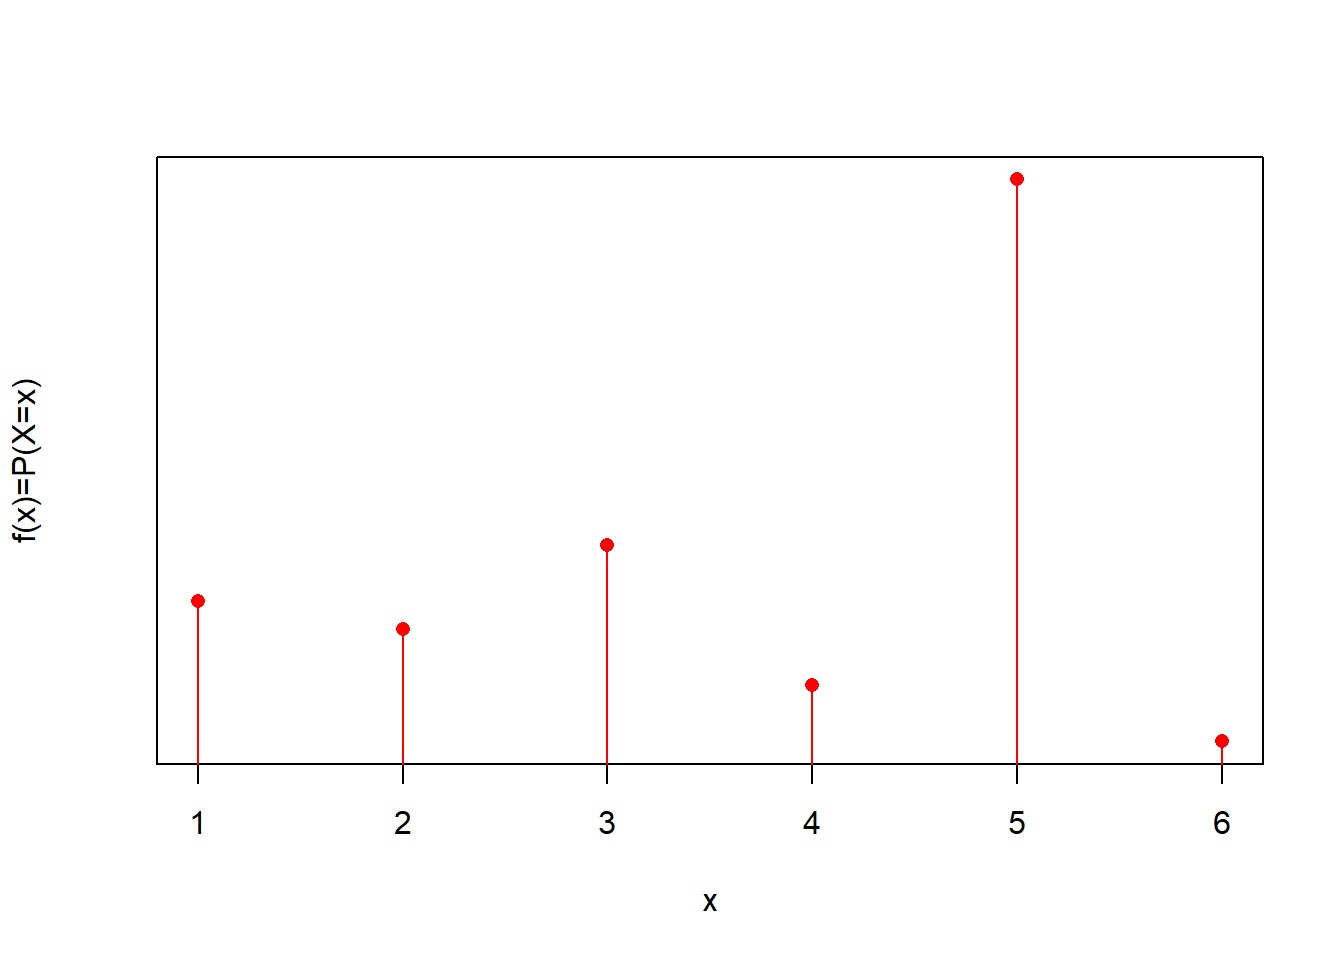
\includegraphics{_main_files/figure-latex/unnamed-chunk-35-1.pdf}

o escrir como una función

\[f(x)=P(X=x)=1/6\]

\hypertarget{funciones-de-probabilidad-1}{%
\section{Funciones de probabilidad}\label{funciones-de-probabilidad-1}}

Podemos \textbf{crear} cualquier tipo de función de probabilidad si satisfacemos las reglas de probabilidad de Kolmogorov:

Para una variable aleatoria discreta \(X \in \{x_1 , x_2 , .. , x_M\}\), una \textbf{función de masa de probabilidad} que se usa para calcular probabilidades

\begin{itemize}
\tightlist
\item
  \(f(x_i)=P(X=x_i)\)
\end{itemize}

siempre es positiva

\begin{itemize}
\tightlist
\item
  \(f(x_i)\geq 0\)
\end{itemize}

y su suma sobre todos los valores de la variable es \(1\):

\begin{itemize}
\tightlist
\item
  \(\sum_{i=1}^M f(x_i)=1\)
\end{itemize}

Donde \(M\) es el número de resultados posibles.

Ten en cuenta que la definición de \(X\) y su función de masa de probabilidad es general \textbf{sin referencia} a ningún experimento. Las funciones viven en el espacio modelo (abstracto).

Aquí tenemos un ejemplo

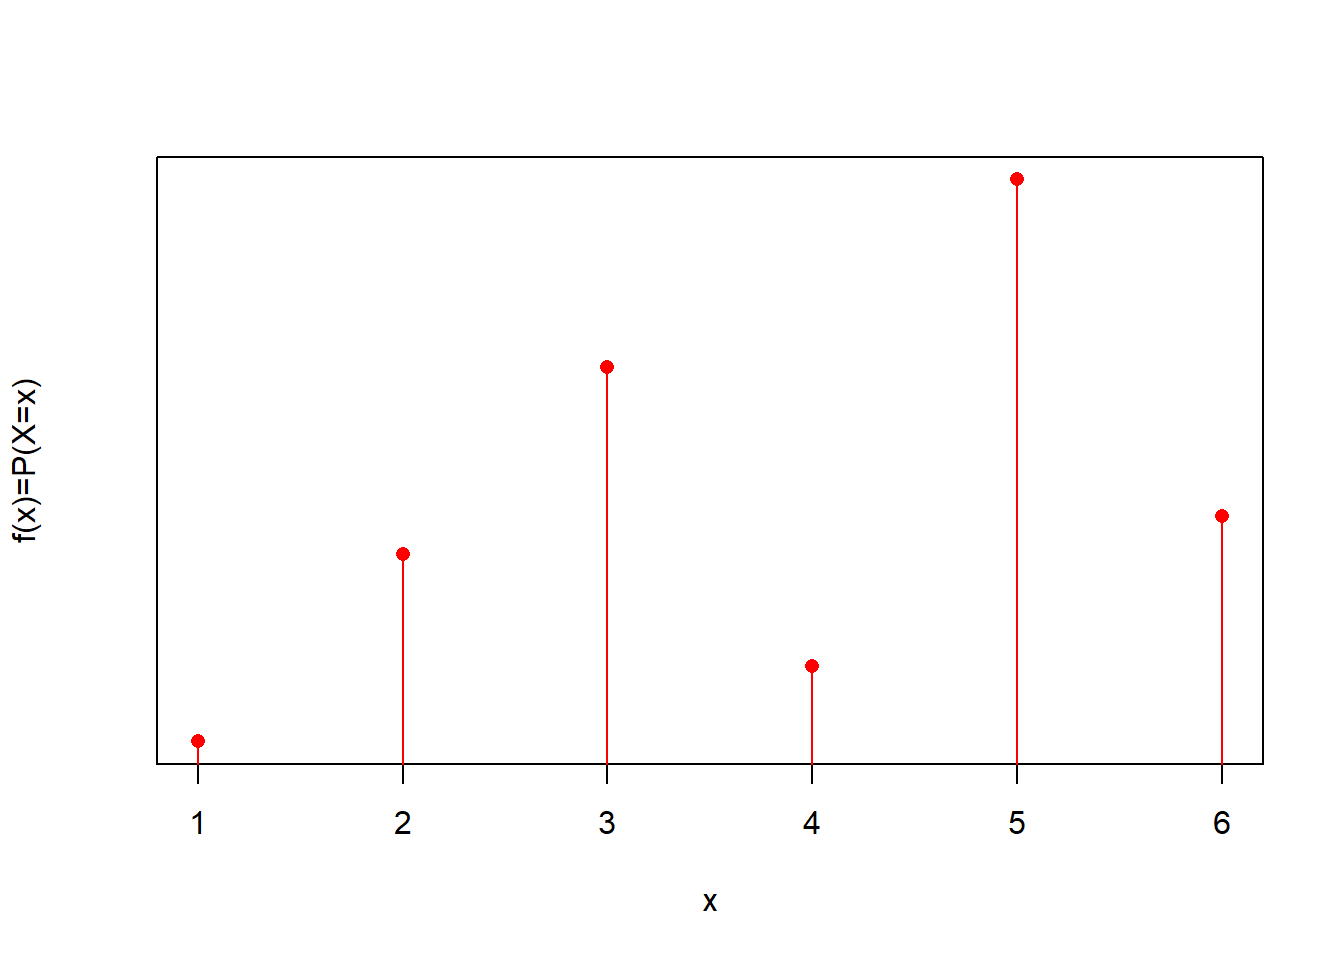
\includegraphics{_main_files/figure-latex/unnamed-chunk-36-1.pdf}

\(X\) y \(f(x)\) son objetos abstractos que pueden corresponder o no a un experimento. Tenemos la libertad de construirlos como queramos siempre que respetemos su definición.

Las funciones de masa de probabilidad tienen algunas \textbf{propiedades} que se derivan exclusivamente de su definición.

\hypertarget{probabilidades-y-frecuencias-relativas}{%
\section{Probabilidades y frecuencias relativas}\label{probabilidades-y-frecuencias-relativas}}

\textbf{Considera el ejemplo}

Haz el siguiente experimento: En una urna pon \(8\) bolas y:

\begin{itemize}
\tightlist
\item
  marca \(1\) bola con el número \(-2\)
\item
  marca \(2\) bolas con el número \(-1\)
\item
  marca \(2\) bolas con el número \(0\)
\item
  marca \(2\) bolas con el número \(1\)
\item
  marca \(1\) bolas con el número \(2\)
\end{itemize}

Y considere realizar el siguiente \textbf{experimento aleatorio:} Tome una bola y lea el número.

A partir de la probabilidad clásica, podemos escribir la tabla de probabilidades, para lo cual no necesitamos realizar ningún experimento

\begin{longtable}[]{@{}cc@{}}
\toprule\noalign{}
\(X\) & \(P(X=x)\) \\
\midrule\noalign{}
\endhead
\bottomrule\noalign{}
\endlastfoot
\(-2\) & \(1/8=0.125\) \\
\(-1\) & \(2/8=0.25\) \\
\(0\) & \(2/8=0.25\) \\
\(1\) & \(2/8=0.25\) \\
\(2\) & \(1/8=0.125\) \\
\end{longtable}

Ahora, realicemos el experimento \(30\) veces y escribamos la tabla de frecuencia

\begin{longtable}[]{@{}cc@{}}
\toprule\noalign{}
\(X\) & \(f_i\) \\
\midrule\noalign{}
\endhead
\bottomrule\noalign{}
\endlastfoot
\(-2\) & \(0.132\) \\
\(-1\) & \(0.262\) \\
\(0\) & \(0.240\) \\
\(1\) & \(0.248\) \\
\(2\) & \(0.118\) \\
\end{longtable}

La probabilidad frecuentista nos dice
\[lim_{N \rightarrow \infty} f_i = f(x_i)=P(X=x_i)\]
Entonces, si no conocíamos el montaje del experimento (caja negra), lo mejor que podemos hacer es \textbf{estimar} las probabilidades con las frecuencias, obtenidas de \(N\) repeticiones del experimento aleatorio:

\[f_i = \hat{P}_i\]

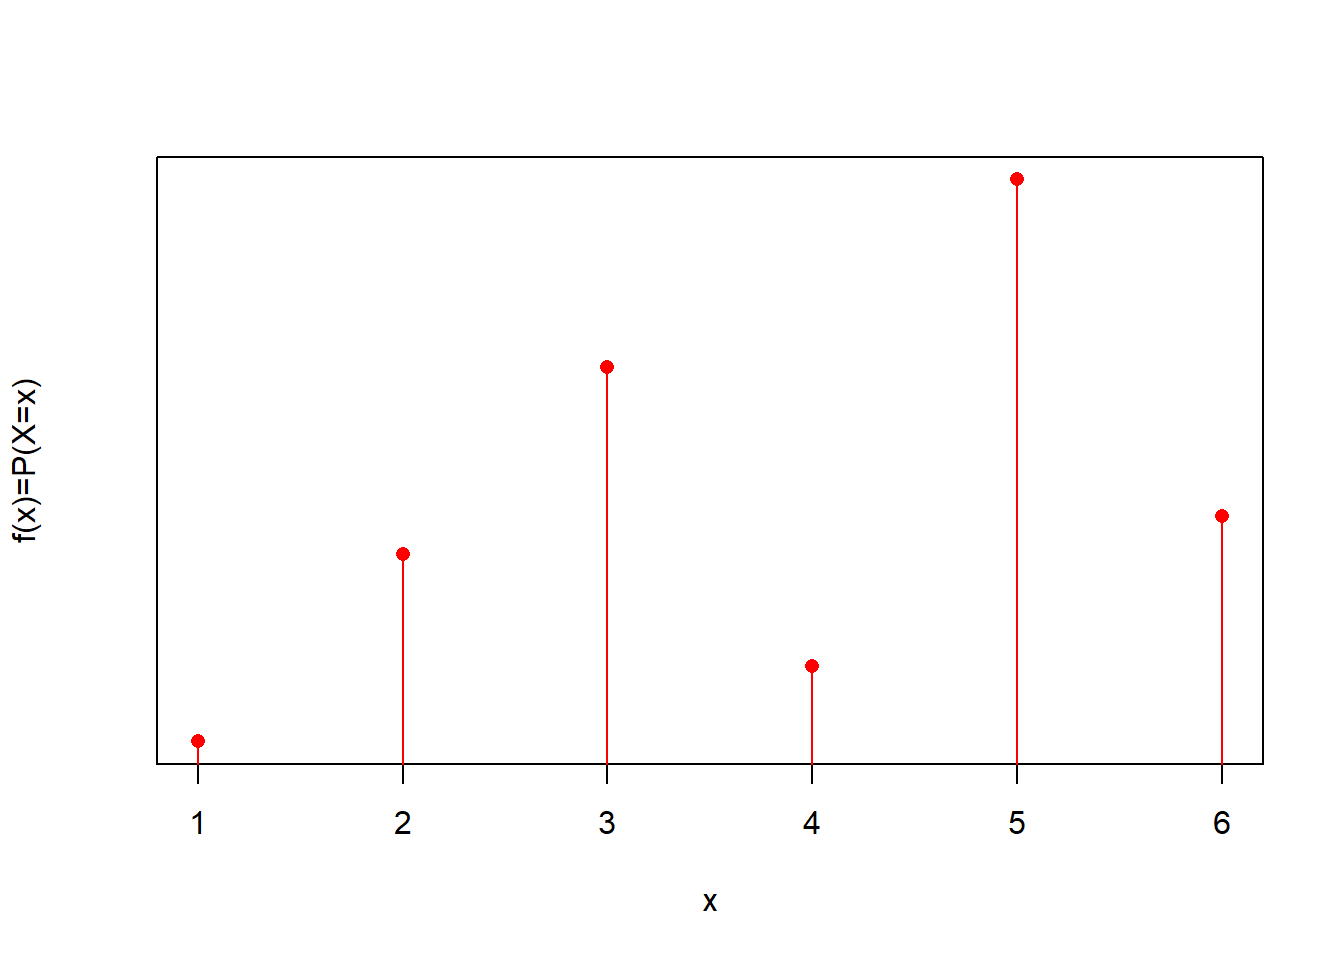
\includegraphics{_main_files/figure-latex/unnamed-chunk-37-1.pdf}

Cada vez que estimamos las probabilidades, nuestras estimaciones \(\hat{P}_i=f_i\) cambian. Pero \(P_i\) es una cantidad abstracta que nunca cambia. A medida que aumenta \(N\), nos acercamos más a ella.

\hypertarget{la-media-o-el-valor-esperado}{%
\section{La media o el valor esperado}\label{la-media-o-el-valor-esperado}}

Cuando discutimos las estadísticas de resumen de los datos, definimos el \textbf{centro} de las observaciones como un valor alrededor del cual se concentran las frecuencias de los resultados.

Usamos el \textbf{promedio} para medir el centro de gravedad de los \textbf{datos}. En términos de las frecuencias relativas de los valores de los resultados discretos, escribimos el promedio como

\(\bar{x}= \sum_{i=1}^M x_i \frac{n_i}{N}=\) \[\sum_{i=1}^M x_i f_i\]

\textbf{Definición}

La \textbf{media} (\(\mu\)) o valor esperado de una variable aleatoria discreta \(X\), \(E(X)\), con función de masa \(f(x)\) está dada por

\[ \mu = E(X)= \sum_{i=1}^M x_i f(x_i) \]

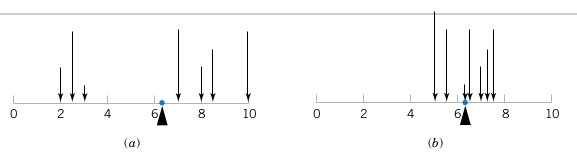
\includegraphics{./figures/mu.png}

Es el centro de gravedad de las \textbf{probabilidades}: El punto donde se equilibran las cargas de probabilidad.

De la definición tenemos

\[\bar{x} \rightarrow \mu\] en el \textbf{límite} cuando
\(N \rightarrow \infty\) como la frecuencia tiende a la función de masa de probabilidad \(f_i \rightarrow f(x_i)\).

\textbf{Ejemplo}

¿Cuál es la media de \(X\) si su función de masa de probabilidad \(f(x)\) está dada por

\begin{longtable}[]{@{}cc@{}}
\toprule\noalign{}
\(X\) & \(f(x)=P(X=x)\) \\
\midrule\noalign{}
\endhead
\bottomrule\noalign{}
\endlastfoot
\(0\) & \(1/16\) \\
\(1\) & \(4/16\) \\
\(2\) & \(6/16\) \\
\(3\) & \(4/16\) \\
\(4\) & \(1/16\) \\
\end{longtable}

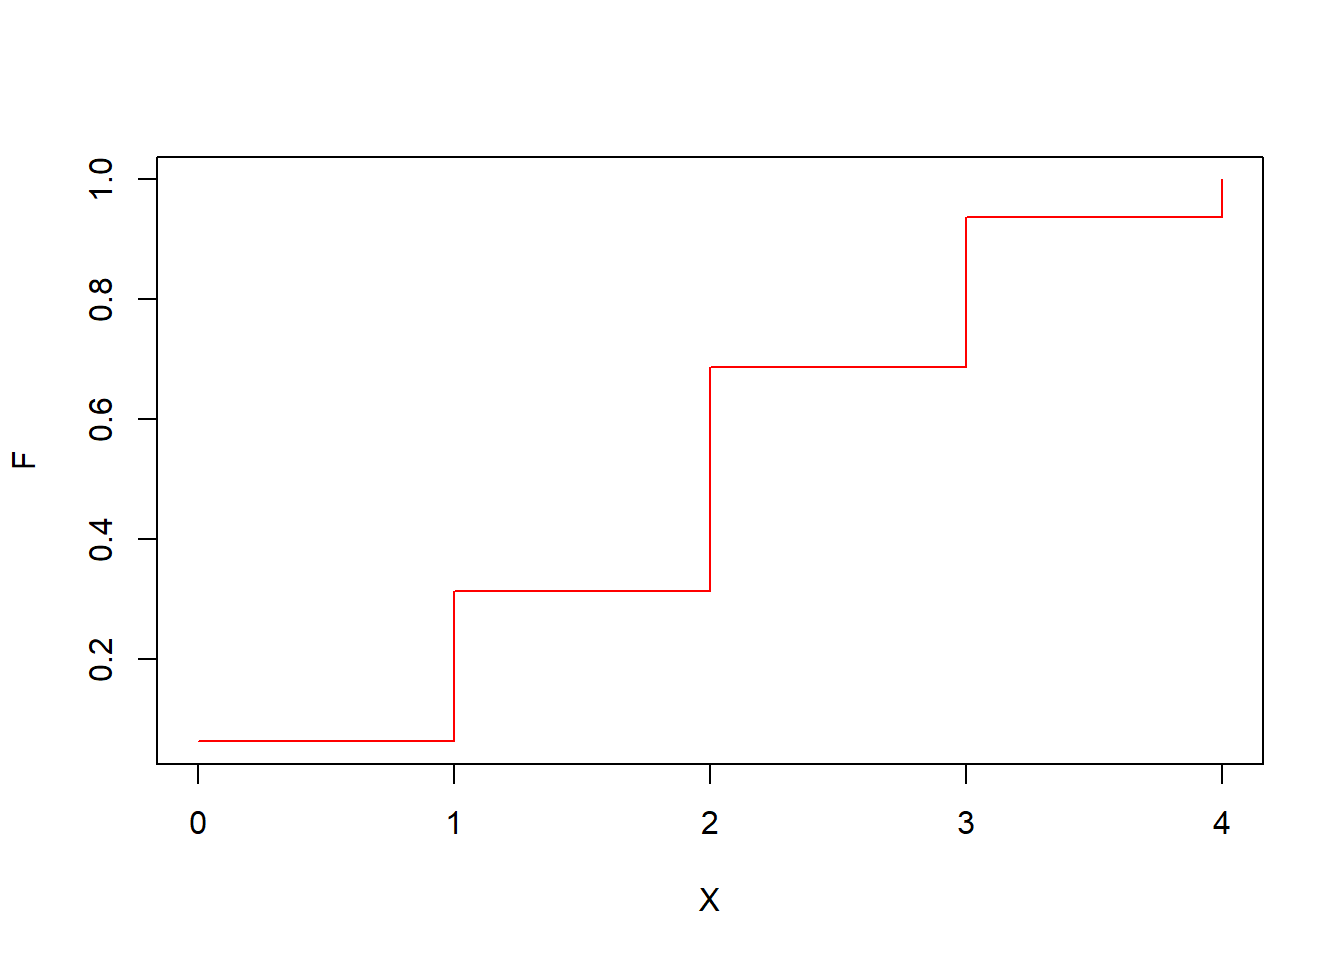
\includegraphics{_main_files/figure-latex/unnamed-chunk-38-1.pdf}

\[ \mu =E(X)=\sum_{i=1}^m x_i f(x_i) \]

\(E(X)=\)\textbf{0} * 1/16 + \textbf{1} * 4/16 + \textbf{2} * 6/16 + \textbf{3} * 4/16 + \textbf{4} * 1/16 =2

La media \(\mu\) es el centro de gravedad de la función de masa de probabilidad y \textbf{no cambia}. Sin embargo, el promedio \(\bar{x}\) es el centro de gravedad de las observaciones (frecuencias relativas) \textbf{cambia} con diferentes datos.

\hypertarget{varianza}{%
\section{Varianza}\label{varianza}}

Cuando discutimos los estadísticos de resumen, también definimos la dispersión de las observaciones como una distancia promedio de los datos al promedio.

\textbf{Definición}

La varianza, escrita como \(\sigma^2\) o \(V(X)\), de una variable aleatoria discreta \(X\) con función de masa \(f(x)\) viene dada por

\[\sigma^2 = V(X)= \sum_{i=1}^M (x_i-\mu)^2 f(x_i)\]
\(\sigma=\sqrt{V(X)}\) se llama la \textbf{desviación estándar} de la variable aleatoria.

La varianza es la dispersión de las \textbf{probabilidades} con respecto a la media: El momento de inercia de las probabilidades sobre la media.

\textbf{Ejemplo}

¿Cuál es la varianza de \(X\) si su función de masa de probabilidad \(f(x)\) está dada por

\begin{longtable}[]{@{}cc@{}}
\toprule\noalign{}
\(X\) & \(f(x)=P(X=x)\) \\
\midrule\noalign{}
\endhead
\bottomrule\noalign{}
\endlastfoot
\(0\) & \(1/16\) \\
\(1\) & \(4/16\) \\
\(2\) & \(6/16\) \\
\(3\) & \(4/16\) \\
\(4\) & \(1/16\) \\
\end{longtable}

\[\sigma^2 =V(X)=\sum_{i=1}^m (x_i-\mu)^2 f(x_i)\]

\(V(X)=\)\textbf{(0-2)}\(^2\)* 1/16 + \textbf{(1-2)}\(^2\)* 4/16 + \textbf{(2- 2)}\(^2\)* 6/16 + \textbf{(3-2)}\(^2\)* 4/16 + \textbf{(4-2)}\(^2\)* 1/ 16 = 1

\[V(X)=\sigma^2=1\]
\[\sigma=1\]

\hypertarget{funciones-de-probabilidad-para-funciones-de-x}{%
\section{\texorpdfstring{Funciones de probabilidad para funciones de \(X\)}{Funciones de probabilidad para funciones de X}}\label{funciones-de-probabilidad-para-funciones-de-x}}

En muchas ocasiones, estaremos interesados en resultados que sean función de las variables aleatorias. Quizás nos interese el cuadrado del número de contagios de gripe, o la raíz cuadrada del número de correos electrónicos en una hora.

\textbf{Definición}

Para cualquier función \(h\) de una variable aleatoria \(X\), con función de masa \(f(x)\), su valor esperado viene dado por

\[ E[h(X)]= \sum_{i=1}^M h(x_i) f(x_i) \]

Esta es una definición importante que nos permite probar tres propiedades de la media y la varianza que se usan con frecuencia:

\begin{enumerate}
\def\labelenumi{\arabic{enumi})}
\item
  La media de una función lineal es la función lineal de la media: \[E(a\times X +b)= a\times E(X) +b\] para \(a\) y \(b\) escalares (números ).
\item
  La varianza de una función lineal de \(X\) es:\[V(a\times X +b)= a^2\times V(X)\]
\item
  La varianza \textbf{con respecto al origen} es la varianza \textbf{con respecto a la media} más la media al cuadrado: \[E(X^2)=V(X)+E(X)^2\]
\end{enumerate}

\textbf{Ejemplo}

¿Cuál es la varianza \(X\) con respecto al origen, \(E(X^2)\), si su función de masa de probabilidad \(f(x)\) está dada por

\begin{longtable}[]{@{}cc@{}}
\toprule\noalign{}
\(X\) & \(f(x)=P(X=x)\) \\
\midrule\noalign{}
\endhead
\bottomrule\noalign{}
\endlastfoot
\(0\) & \(1/16\) \\
\(1\) & \(4/16\) \\
\(2\) & \(6/16\) \\
\(3\) & \(4/16\) \\
\(4\) & \(1/16\) \\
\end{longtable}

\[E(X^2) =\sum_{i=1}^m x_i^2 f(x_i)\]

\(E(X^2)=\)\textbf{(0)}\(^2\)* 1/16 + \textbf{(1)}\(^2\)* 4/16 + \textbf{(2)} \(^2\)* 6/16 + \textbf{(3)}\(^2\)* 4/16 + \textbf{(4)}\(^2\)* 1/16 =5

También podemos verificar:

\[E(X^2)=V(X)+E(X)^2\]

\(5=1+2^2\)

\hypertarget{distribuciuxf3n-de-probabilidad}{%
\section{Distribución de probabilidad}\label{distribuciuxf3n-de-probabilidad}}

Cuando discutimos las estadísticas de resumen, también definimos la \textbf{distribución} de frecuencias (o la frecuencia acumulada relativa) \(F_i\). \(F_i\) es una cantidad importante porque es una función continua \(F_x\) es por lo tanto una función de rango \textbf{continuo}, incluso si los resultados son discretos.

\textbf{Definición:}

La función de \textbf{distribución de probabilidad} se define como

\[F(x)=P(X\leq x)=\sum_{x_i\leq x} f(x_i) \]

Esa es la probabilidad acumulada hasta un valor dado \(x\)

\(F(x)\) satisface por lo tanto satisface:

\begin{enumerate}
\def\labelenumi{\arabic{enumi})}
\tightlist
\item
  \(0\leq F(x) \leq 1\)
\item
  Si \(x \leq y\), entonces \(F(x) \leq F(y)\)
\end{enumerate}

Para la función de masa de probabilidad:

\begin{longtable}[]{@{}cc@{}}
\toprule\noalign{}
\(X\) & \(f(x)=P(X=x)\) \\
\midrule\noalign{}
\endhead
\bottomrule\noalign{}
\endlastfoot
\(0\) & \(1/16\) \\
\(1\) & \(4/16\) \\
\(2\) & \(6/16\) \\
\(3\) & \(4/16\) \\
\(4\) & \(1/16\) \\
\end{longtable}

La distribución de probabilidad es:

\[
    F(x)=
\begin{cases}
    1/16,& \text{if } 0 \leq x < 1\\
    5/16,& 1\leq x < 2\\
    11/16,& 2\leq x < 3\\
    15/16,& 4\leq x < 5\\
    16/16,&  x \leq 5\\
\end{cases}
\]

Para \(X \in \mathbb{Z}\)

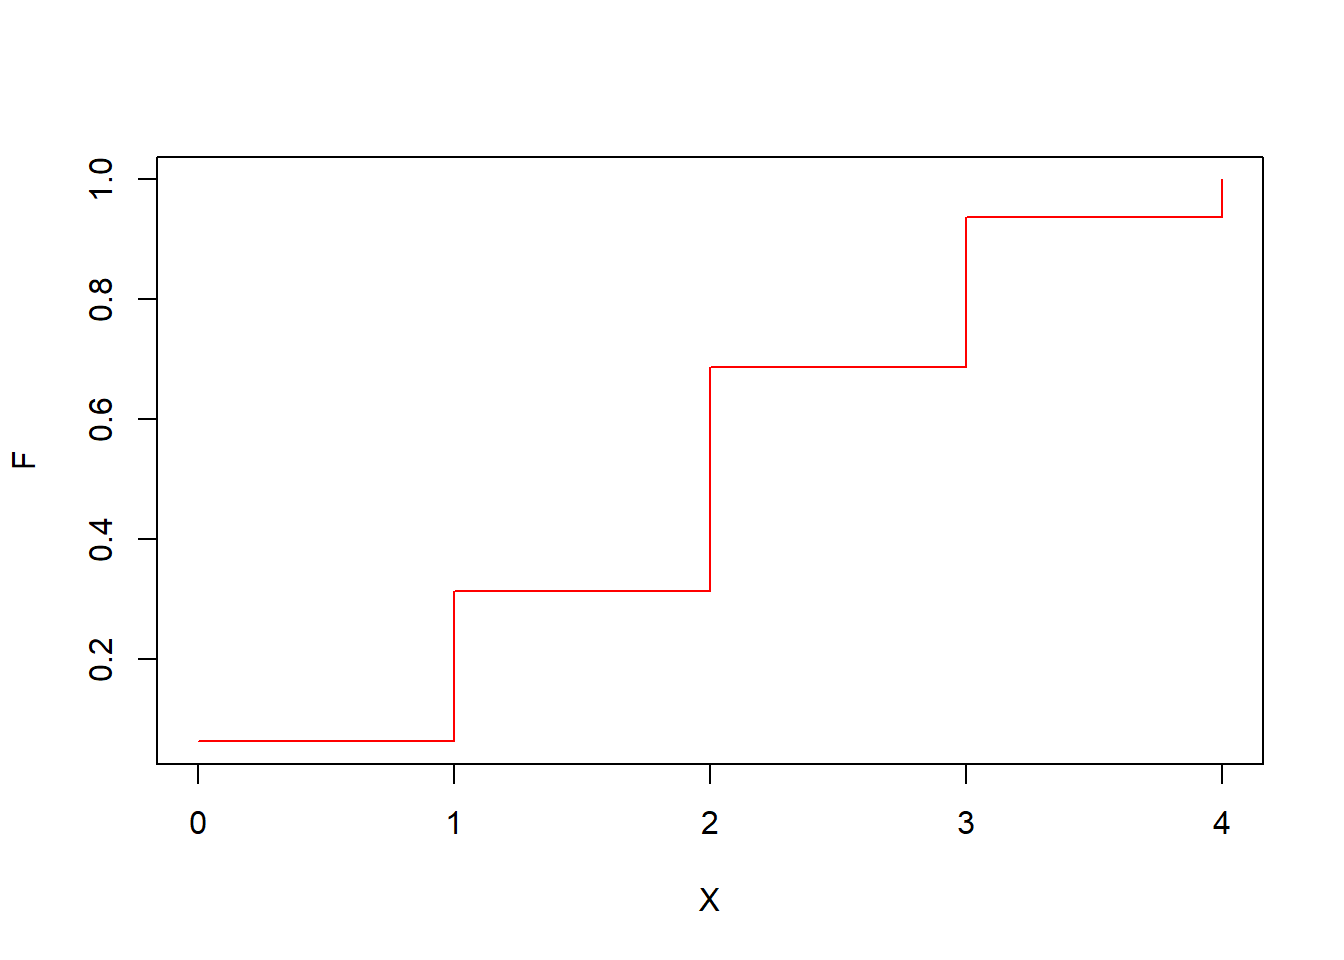
\includegraphics{_main_files/figure-latex/unnamed-chunk-39-1.pdf}

\hypertarget{funciuxf3n-de-probabilidad-y-distribuciuxf3n-de-probabilidad}{%
\section{Función de probabilidad y distribución de probabilidad}\label{funciuxf3n-de-probabilidad-y-distribuciuxf3n-de-probabilidad}}

La función de probabilidad y la distribución son equivalentes. Podemos obtener uno del otro y viceversa.

\[f(x_i)=F(x_i)-F(x_{i-1})\]

con

\[f(x_1)=F(x_1)\]

para \(X\) tomando valores en \(x_1 \leq x_2 \leq ... \leq x_n\)

\textbf{Ejemplo}

De la distribución de probabilidad:

\[
    F(x)=
\begin{cases}
    1/16,& \text{if } 0 \leq x < 1\\
    5/16,& 1\leq x < 2\\
    11/16,& 2\leq x < 3\\
    15/16,& 4\leq x < 5\\
    16/16,&  x \leq 5\\
\end{cases}
\]

Podemos obtener la función masa de probabilidad.

\(f(0)=F(0)=1/16\)
\(f(1)=F(1)-f(0)=5/32-1/32=4/16\)
\(f(2)=F(2)-f(1)-f(0)=F(2)-F(1)=6/16\)
\(f(3)=F(3)-f(2)-f(1)-f(0)=F(3)-F(2)=4/16\)
\(f(4)=F(4)-F(3)=1/16\)

\hypertarget{cuantiles}{%
\section{Cuantiles}\label{cuantiles}}

Finalmente, podemos usar la distribución de probabilidad \(F(x)\) para definir la mediana y los cuartiles de la variable aleatoria \(X\).

En general, definimos el \textbf{q-cuantil} como el valor \(x_{p}\) \textbf{bajo} el cual hemos acumulado q*100\% de la probabilidad

\[q=\sum_{i=1}^pf(x_i) = F (x_p)\]

\begin{itemize}
\tightlist
\item
  La \textbf{mediana} es valor \(x_m\) tal que \(q=0.5\)
\end{itemize}

\[F(x_{m})=0.5\]

\begin{itemize}
\tightlist
\item
  El cuantil \(0.05\) es el valor \(x_{r}\) tal que \(q=0.05\)
\end{itemize}

\[F(x_{r})=0.05\]

\begin{itemize}
\tightlist
\item
  El cuantil de \(0,25\) es el \textbf{primer cuartil} el valor \(x_{s}\) tal que \(q=0.25\)
\end{itemize}

\[F(x_{s})=0.25\]

\hypertarget{resumen}{%
\section{Resumen}\label{resumen}}

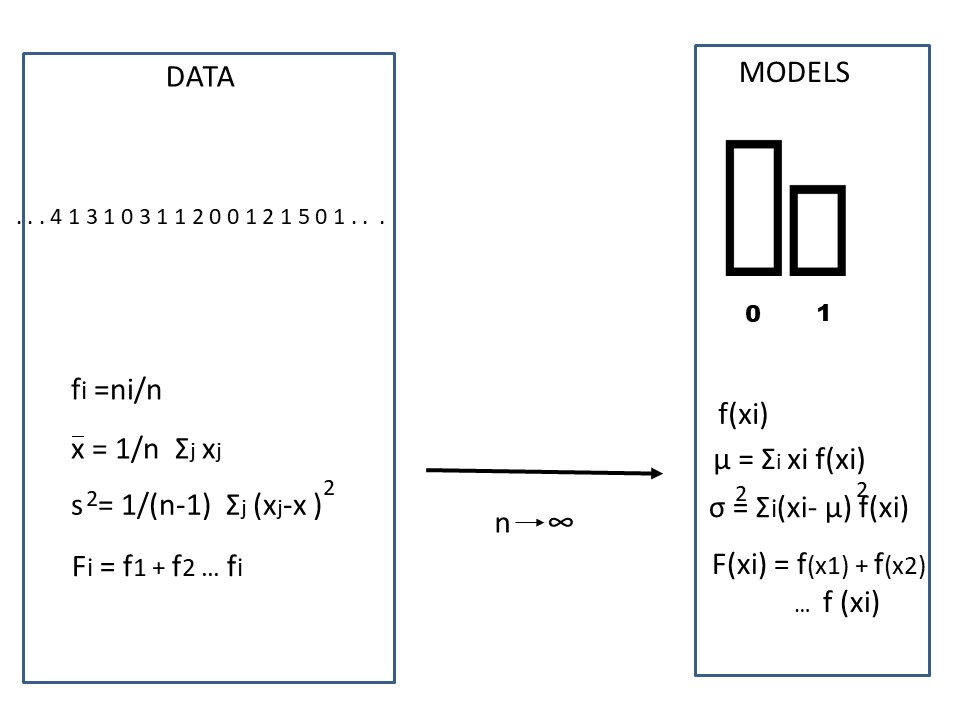
\includegraphics{./figures/randomvarsum.JPG}

\begin{longtable}[]{@{}
  >{\centering\arraybackslash}p{(\columnwidth - 4\tabcolsep) * \real{0.4348}}
  >{\centering\arraybackslash}p{(\columnwidth - 4\tabcolsep) * \real{0.3043}}
  >{\centering\arraybackslash}p{(\columnwidth - 4\tabcolsep) * \real{0.2609}}@{}}
\toprule\noalign{}
\begin{minipage}[b]{\linewidth}\centering
nombres de cantidades
\end{minipage} & \begin{minipage}[b]{\linewidth}\centering
modelo (no observado)
\end{minipage} & \begin{minipage}[b]{\linewidth}\centering
datos (observados)
\end{minipage} \\
\midrule\noalign{}
\endhead
\bottomrule\noalign{}
\endlastfoot
función de masa de probabilidad // frecuencia relativa & \(f(x_i)=P(X=x_i)\) & \(f_i=\frac{n_i}{N}\) \\
distribución de probabilidad // frecuencia relativa acumulada & \(F(x_i)=P(X \leq x_i)\) & \(F_i=\sum_{k\leq i} f_k\) \\
media // promedio & \(\mu=E(X)=\sum_{i=1}^M x_i f(x_i)\) & \(\bar{x}=\sum_{j=1}^N x_j/N\) \\
varianza // varianza de la muestra & \(\sigma^2=V(X)=\sum_{i=1}^M (x_i-\mu)^2 f(x_i)\) & \(s^2=\sum_{j=1}^N (x_j-\bar{x})^2/(N-1)\) \\
desviación estándar // muestra sd & \(\sigma=\sqrt{V(X)}\) & \(s\) \\
varianza con respecto al origen // 2º momento muestral & \(E(X^2)=\sum_{i=1}^M x_i^2 f(x_i)\) & \(m_2= \sum_{j=1}^N x_j^2/n\) \\
\end{longtable}

Ten en cuenta:

\begin{itemize}
\tightlist
\item
  \(i=1...M\) es un \textbf{resultado} de la variable aleatoria \(X\).
\item
  \(j=1...N\) es una \textbf{observación} de la variable aleatoria \(X\).
\end{itemize}

Propiedades:

\begin{itemize}
\tightlist
\item
  \(\sum_{i=1...N} f(x_i)=1\)
\item
  \(f(x_i)=F(x_i)-F(x_{i-1})\)
\item
  \(E(a\times X +b)= a\times E(X) +b\); for \(a\) and \(b\) scalars.
\item
  \(V(a\times X +b)= a^2\times V(X)\)
\item
  \(E(X^2)=V(X)+E(X)^2\)
\end{itemize}

\hypertarget{preguntas-3}{%
\section{Preguntas}\label{preguntas-3}}

\textbf{1)} Para una función de masa de probabilidad no es cierto que

\textbf{\(\qquad\)a:} la suma de los valores de su imagen es 1; \textbf{\(\qquad\)b:} sus valores pueden interpretarse como probabilidades de eventos;
\textbf{\(\qquad\)c:} siempre es positiva;
\textbf{\(\qquad\)d:} no puede tomar el valor 1;

\textbf{2)} El valor de una variable aleatoria representa

\textbf{\(\qquad\)a:} una observación de un experimento aleatorio; \textbf{\(\qquad\)b:} la frecuencia de un resultado de un experimento aleatorio;
\textbf{\(\qquad\)c:} un resultado de un experimento aleatorio;
\textbf{\(\qquad\)d:} una probabilidad de un resultado;

\textbf{3)} El valor estimado de una probabilidad \(\hat{P_i}\) es igual a la probabilidad \(P_i\) cuando el número de repeticiones del experimento aleatorio es

\textbf{\(\qquad\)a:} grande; \textbf{\(\qquad\)b:} infinito;
\textbf{\(\qquad\)c:} pequeño
\textbf{\(\qquad\)d:} cero;

\textbf{4)} Si una función de masa de probabilidad es simétrica alrededor de \(x=0\)

\textbf{\(\qquad\)a:} La media es menor que la mediana; \textbf{\(\qquad\)b:} La media es mayor que la mediana;
\textbf{\(\qquad\)c:} La media y la mediana son iguales;
\textbf{\(\qquad\)d:} La media y la mediana son diferentes de 0;

\textbf{5)} La media y la varianza

\textbf{\(\qquad\)a:} son inversamente proporcionales; \textbf{\(\qquad\)b:} son valores esperados de funciones de \(X\);
\textbf{\(\qquad\)c:} de una función lineal son la función lineal de la media y la función lineal de la varianza;
\textbf{\(\qquad\)d:} cambia cuando repetimos el experimento aleatorio;

\hypertarget{ejercicios-3}{%
\section{Ejercicios}\label{ejercicios-3}}

\hypertarget{ejercicio-1-2}{%
\subsubsection{Ejercicio 1}\label{ejercicio-1-2}}

Ponemos en una urna papeletas con letras de la a la f.~Considera el sorteo que da \(0\) euros a las dos primeras letras del abecedario, \(1.5\) euros a las dos siguientes, y \(2\) y \(3\) euros a las siguientes.

\begin{enumerate}
\def\labelenumi{\alph{enumi})}
\item
  ¿cuál es la función de masa de probabilidad y función de distribución de probabilidad de para los premios en dinero del juego?
\item
  ¿cuál es el valor esperado del premio? (R:1.3)
\item
  ¿cuál es la varianza del premio? (R:1.13)
\item
  ¿cuál es la probabilidad de ganar 2 o mas euros? (R:2/6)
\end{enumerate}

\hypertarget{ejercicio-2-2}{%
\subsubsection{Ejercicio 2}\label{ejercicio-2-2}}

Dada la función de masa de probabilidad

\begin{longtable}[]{@{}cc@{}}
\toprule\noalign{}
\(x\) & \(f(x)=P(X=x)\) \\
\midrule\noalign{}
\endhead
\bottomrule\noalign{}
\endlastfoot
10 & 0.1 \\
12 & 0.3 \\
14 & 0.25 \\
15 & 0.15 \\
17 & ? \\
20 & 0.15 \\
\end{longtable}

\begin{itemize}
\tightlist
\item
  ¿Cuál es su valor esperado y su desviación estándar? (R: 14,2; 2,95)
\end{itemize}

\hypertarget{ejercicio-3-2}{%
\subsubsection{Ejercicio 3}\label{ejercicio-3-2}}

Dada la distribución de probabilidad para una variable discreta \(X\)

\[
    F(x)= 
\begin{cases}
0, & x < -1 \\
0.2,& x \in [-1,0)\\
0.35,& x \in [0,1)\\
0.45,& x \in [1,2)\\
1,& x \geq 2\\
\end{cases}
\]

\begin{itemize}
\tightlist
\item
  encuentra \(f(x)\)
\item
  encuentra \(E(X)\) y \(V(X)\) (R:1; 1.5)
\item
  cuál es el valor esperado y la varianza de \(Y=2X+3\) (R:5, 6)
\item
  ¿Cuál es la mediana y el primer y tercer cuartil de \(X\)? (R:2,0,2)
\end{itemize}

\hypertarget{ejercicio-4-1}{%
\subsubsection{Ejercicio 4}\label{ejercicio-4-1}}

Estamos probando un sistema para transmitir imágenes digitales. Primero consideramos el experimento de enviar \(3\) píxeles y tener como resultados \textbf{posibles} eventos como \((0,1,1)\). Este es el evento de recibir el primer píxel sin error, el segundo con error y el tercero con error.

\begin{itemize}
\item
  Enumera en una columna el espacio muestral del experimento aleatorio.
\item
  En la segunda columna asigna la variable aleatoria que cuenta el número de errores transmitidos para cada resultado
\end{itemize}

Considera que tenemos un canal totalmente ruidoso, es decir, cualquier resultado de tres píxeles es igualmente probable.

\begin{itemize}
\item
  ¿Cuál es la probabilidad de recibir errores de \(0\), \(1\), \(2\) o \(3\) en la transmisión de \(3\) píxeles? (R: 1/8; 3/8; 3/8; 1/8)
\item
  Dibuja la función de masa de probabilidad para el número de errores
\item
  ¿Cuál es el valor esperado para el número de errores? (R:1.5)
\item
  ¿Cuál es su varianza? (R: 0,75)
\item
  Dibuja la distribución de probabilidad
\item
  ¿Cuál es la probabilidad de transmitir al menos 1 error? (R:7/8)
\end{itemize}

\hypertarget{variables-aleatorias-continuas}{%
\chapter{Variables aleatorias continuas}\label{variables-aleatorias-continuas}}

\hypertarget{objetivo-2}{%
\section{Objetivo}\label{objetivo-2}}

En este capítulo estudiaremos variables aleatorias continuas.

Definiremos la función de densidad de probabilidad, su media y varianza. De forma similar a las variables aleatorias discretas, definiremos la función de distribución de probabilidad.

\hypertarget{variables-aleatorias-continuas-1}{%
\section{Variables aleatorias continuas}\label{variables-aleatorias-continuas-1}}

En el capítulo pasado usamos las probabilidades de variables aleatorias discretas para definir la función de masa de probabilidad \[f(x)=P(X= x)\]

Donde la probabilidad de que la variable aleatoria tome el valor \(x\) la entendemos como el valor de su frecuencia relativa, cuando el número de repeticiones del experimiento aleatorio tiende a infinito.

Cuando hablamos de datos continous vimos que teníamos que transformarlos en variables discretas (bins) para producir tablas de frecuencias relativas o histogramas. Veamos cómo definir las probabilidades de las variables continuas teniendo en cuenta estas particiones.

\textbf{Ejemplo (misofonía)}

Reconsideremos el ángulo de convexidad de los pacientes con misofonía (Sección 2.21). El ángulo de convexidas de 123 pacientes fue medido. Entendimos cada medición como el resultado de un experimento aleatorio que repetimos 123 veces y que podíamos describir en una tabla de frecuencias o en un histograma.

Para hacer esto, redefinimos los resultados como pequeños intervalos regulares (bins) y calculamos la frecuencia relativa de cada intervalo.

\begin{verbatim}
##        outcome ni         fi
## 1 [-1.02,3.46]  8 0.06504065
## 2  (3.46,7.92] 51 0.41463415
## 3  (7.92,12.4] 26 0.21138211
## 4  (12.4,16.8] 20 0.16260163
## 5  (16.8,21.3] 18 0.14634146
\end{verbatim}

\hypertarget{frecuencias-relativas-3}{%
\section{frecuencias relativas}\label{frecuencias-relativas-3}}

Por lo tanto, definimos la probabilidad de observar un intervalo \(i\) como la frecuencia relativa del intervalo cuando \(N \rightarrow \infty\)

\[ f_i =\frac{ n_ i }{ N} \rightarrow P( x_i \leq X \leq x_i + \Delta x)\]

Esta probabilidad depende de la longitud de los bins \(\Delta x\).

Si hacemos los bins cada vez más pequeños, las frecuencias se hacen más pequeñas y, por lo tanto,

\[P(x_i \leq X \leq x_i + \Delta x) \rightarrow 0\] cuando \(\Delta x \rightarrow 0\) porque \(n_i \rightarrow 0\)

Veamos cómo las frecuencias relativas se hacen más pequeñas cuando dividimos el rango de \(X\) en \(20\) bins

\begin{verbatim}
##          outcome ni         fi
## 1  [-1.02,0.115]  2 0.01626016
## 2   (0.115,1.23]  0 0.00000000
## 3    (1.23,2.34]  3 0.02439024
## 4    (2.34,3.46]  3 0.02439024
## 5    (3.46,4.58]  2 0.01626016
## 6    (4.58,5.69]  4 0.03252033
## 7     (5.69,6.8] 11 0.08943089
## 8     (6.8,7.92] 34 0.27642276
## 9    (7.92,9.04] 12 0.09756098
## 10   (9.04,10.2]  4 0.03252033
## 11   (10.2,11.3]  3 0.02439024
## 12   (11.3,12.4]  7 0.05691057
## 13   (12.4,13.5]  2 0.01626016
## 14   (13.5,14.6]  6 0.04878049
## 15   (14.6,15.7]  4 0.03252033
## 16   (15.7,16.8]  8 0.06504065
## 17     (16.8,18]  4 0.03252033
## 18     (18,19.1]  9 0.07317073
## 19   (19.1,20.2]  3 0.02439024
## 20   (20.2,21.3]  2 0.01626016
\end{verbatim}

\hypertarget{funciuxf3n-de-densidad-de-probabilidad}{%
\section{función de densidad de probabilidad}\label{funciuxf3n-de-densidad-de-probabilidad}}

Definimos una cantidad en un punto \(x\) que es \textbf{la probabilidad por unidad de distancia} de que una observación esté en el bin \textbf{infinitesimal} entre \(x\) y \(x+dx\)

\[f(x)= \frac{ P(x\leq X \leq x+dx )}{dx}\]

\(f(x)\) se llama la \textbf{función de densidad de probabilidad}.

Por lo tanto, la probabilidad de observar \(X\) entre \(x\) y \(x+dx\)
está dada por

\[P( x\leq X \leq x+dx )= f(x) dx\]

\textbf{Definición}

Para una variable aleatoria continua \(X\), una función de \textbf{densidad de probabilidad} es tal que

\begin{enumerate}
\def\labelenumi{\arabic{enumi})}
\tightlist
\item
  Es positiva:
\end{enumerate}

\[f(x) \geq 0\]

\begin{enumerate}
\def\labelenumi{\arabic{enumi})}
\setcounter{enumi}{1}
\tightlist
\item
  La probabilidad de observar \textbf{cualquier} valor de \(x\) es 1:
\end{enumerate}

\[\int_{-\infty}^{\infty} f(x) dx = 1\]

\begin{enumerate}
\def\labelenumi{\arabic{enumi})}
\setcounter{enumi}{2}
\tightlist
\item
  La probabilidad de observar un valor dentro de un intervalo es el \textbf{área bajo la curva}:
\end{enumerate}

\[ P( a\leq X \leq b)=\int_{a}^{b} f(x) dx\]

Las propiedades aseguran que \(f(x)dx\) satisfacen las propiedades de probabilidad de Kolmogorov.

La función de densidad de probabilidad es un paso más en la abstracción de probabilidades en la que añadimos el límite continuo

\[dx \rightarrow 0\]

Todas las propiedades de las probabilidades se traducen en términos de densidades y por lo tanto cambiamos sumatorios por integrales

\[\sum \rightarrow \int\]

Las densidades de probabilidad son cantidades matemáticas que no necesariamente representan experimientos aleatorios.

Un interés fundamental en estadística es describir las densidades que describen nuestro experimento aleatorio concreto.

\hypertarget{uxe1rea-total-bajo-la-curva}{%
\section{Área total bajo la curva}\label{uxe1rea-total-bajo-la-curva}}

\textbf{Ejemplo (gotas de lluvia)}

tomemos una \textbf{densidad de probabilidad} que podría describir la variable aleatoria que mide dónde cae una gota de lluvia en una canaleta de \(100\) cm de longitud.

\[
    f(x)= 
\begin{cases}
    \frac{1}{100},& \text{si } x\in (0,100)\\
    0,& de\, otra\, forma 
\end{cases}
\]

Verifiquemos que la función satisface las tres propiedades de una densidad de probabilidad.

\begin{enumerate}
\def\labelenumi{\arabic{enumi})}
\item
  es evidente a partir de la definición que \(f(x) \geq 0\)
\item
  La probabilidad de observar \textbf{cualquier valor} de \(X\) es el \textbf{área total bajo la curva}
\end{enumerate}

\(P( -\infty \leq X \leq \infty )= \int_{-\infty }^{\infty } f(x) dx = 100*0.01= 1\)

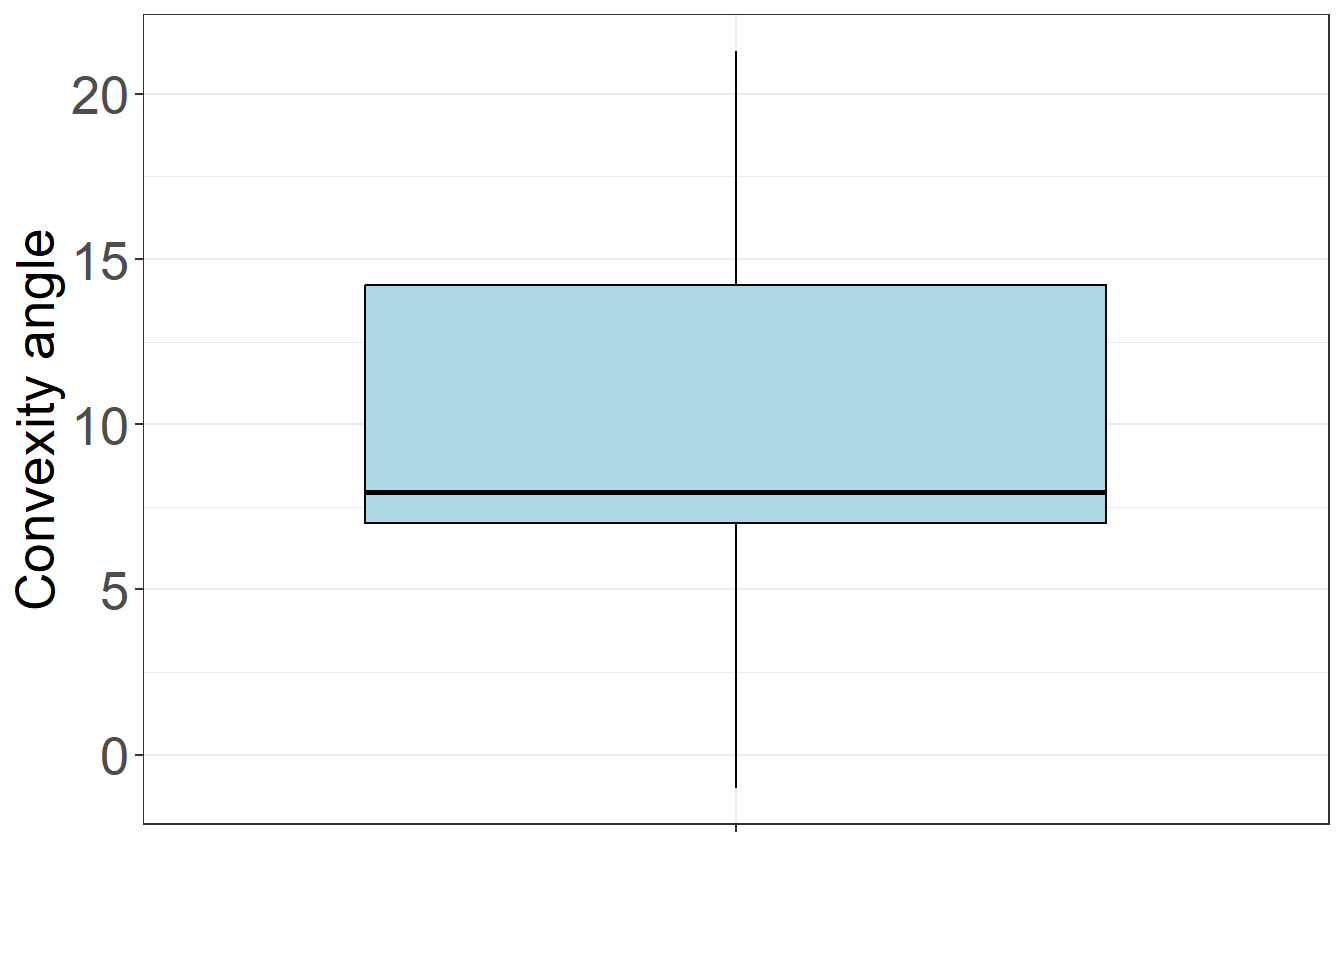
\includegraphics{_main_files/figure-latex/unnamed-chunk-42-1.pdf}

\begin{enumerate}
\def\labelenumi{\arabic{enumi})}
\setcounter{enumi}{2}
\tightlist
\item
  La probabilidad de observar \(X\) en un intervalo es el \textbf{área bajo la curva} dentro del intervalo
\end{enumerate}

\begin{itemize}
\tightlist
\item
  \(P( 20 \leq X \leq 60) = \int_{20}^{60} f(x) dx = (60-20)*0.01=0.4\)
\end{itemize}

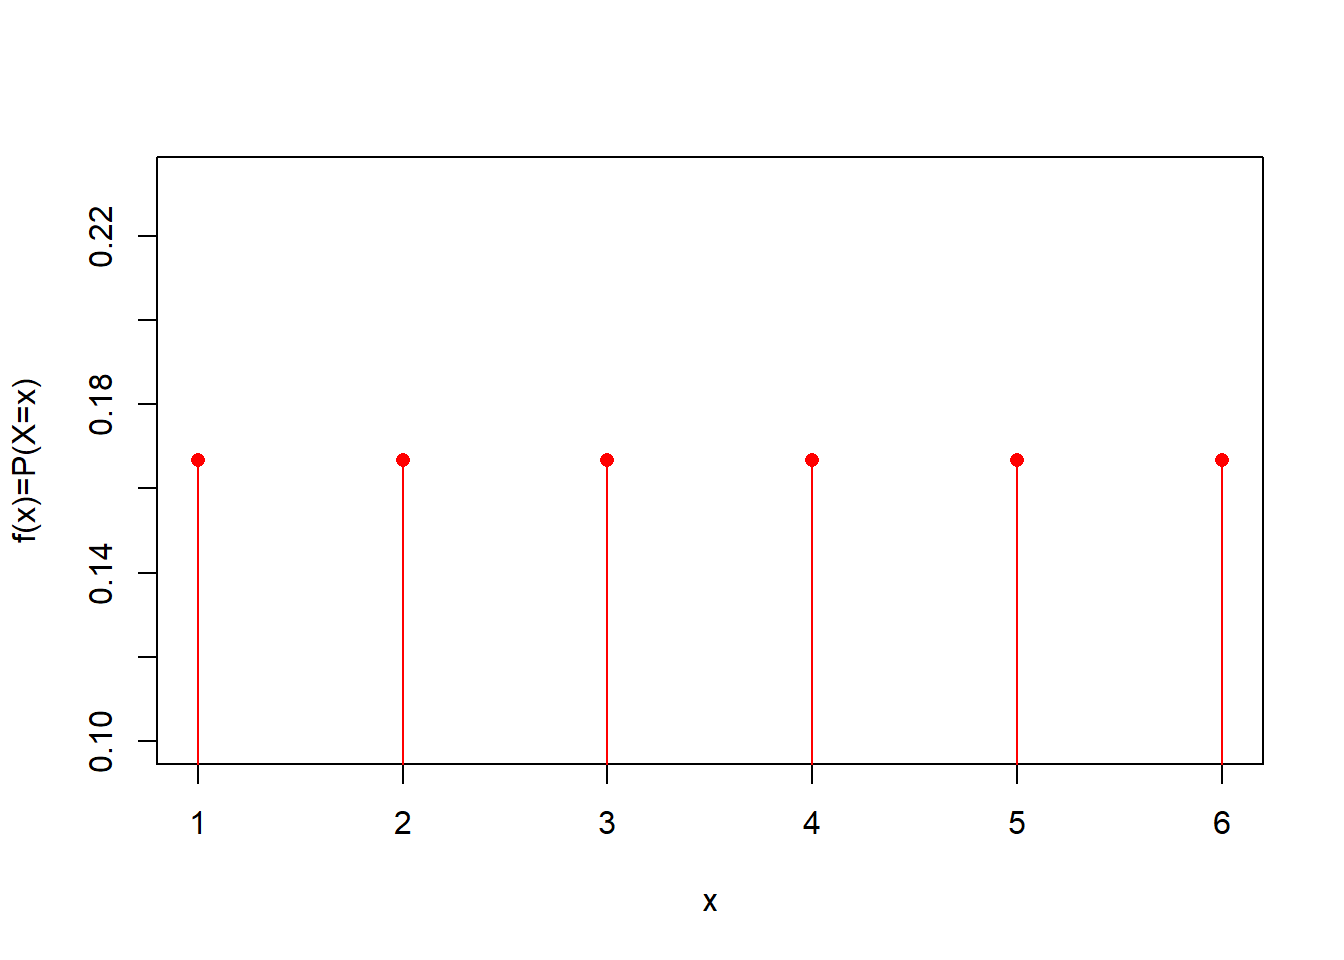
\includegraphics{_main_files/figure-latex/unnamed-chunk-43-1.pdf}

\hypertarget{probabilidades-de-variables-continuas}{%
\section{Probabilidades de variables continuas}\label{probabilidades-de-variables-continuas}}

Para variables continuas, calculamos la probabilidad de que la variable esté en un intervalo dado. Eso es

\[P( a \leq X \leq b)\]
Recordemos que para variables continuas, la probabilidad de que el experimento nos dé un número real particular es cero: \(P(X= a)= 0\)

La probabilidad \(P( a \leq X \leq b)\) es el área bajo la curva de \(f(x)\) entre \(a\) y \(b\)

\begin{itemize}
\tightlist
\item
  \(P( a \leq X \leq b) = \int_{a}^{b} f(x) dx\)
\end{itemize}

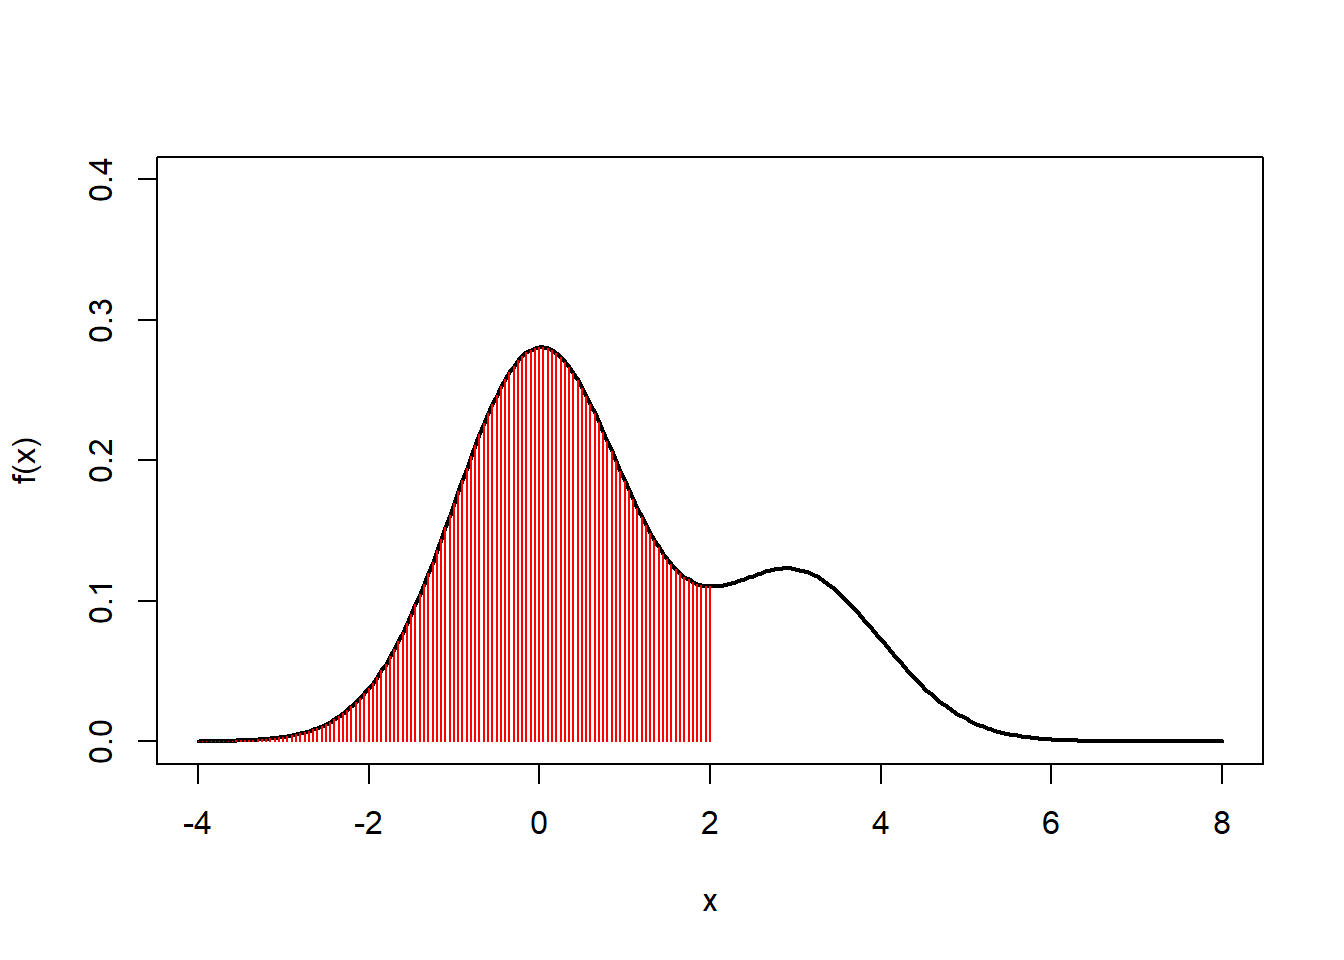
\includegraphics{_main_files/figure-latex/unnamed-chunk-44-1.pdf}

\hypertarget{distribuciuxf3n-de-probabilidad-1}{%
\section{Distribución de probabilidad}\label{distribuciuxf3n-de-probabilidad-1}}

La \textbf{distribución de probabilidad} \(F(c)\) definida como la acumulación de probabilidad hasta el resultado \(C\)

\(F(c) = P( X \leq c)\)

se puede utilizar para calcular la probabilidad \(P( a \leq X \leq b)\).

Si consideramos que:

\begin{enumerate}
\def\labelenumi{\arabic{enumi})}
\tightlist
\item
  la probabilidad acumulada hasta \(b\) está dada por
\end{enumerate}

\begin{itemize}
\tightlist
\item
  \(F(b) = P( X \leq b)=\int_{-\infty }^bf(x)dx\)
\end{itemize}

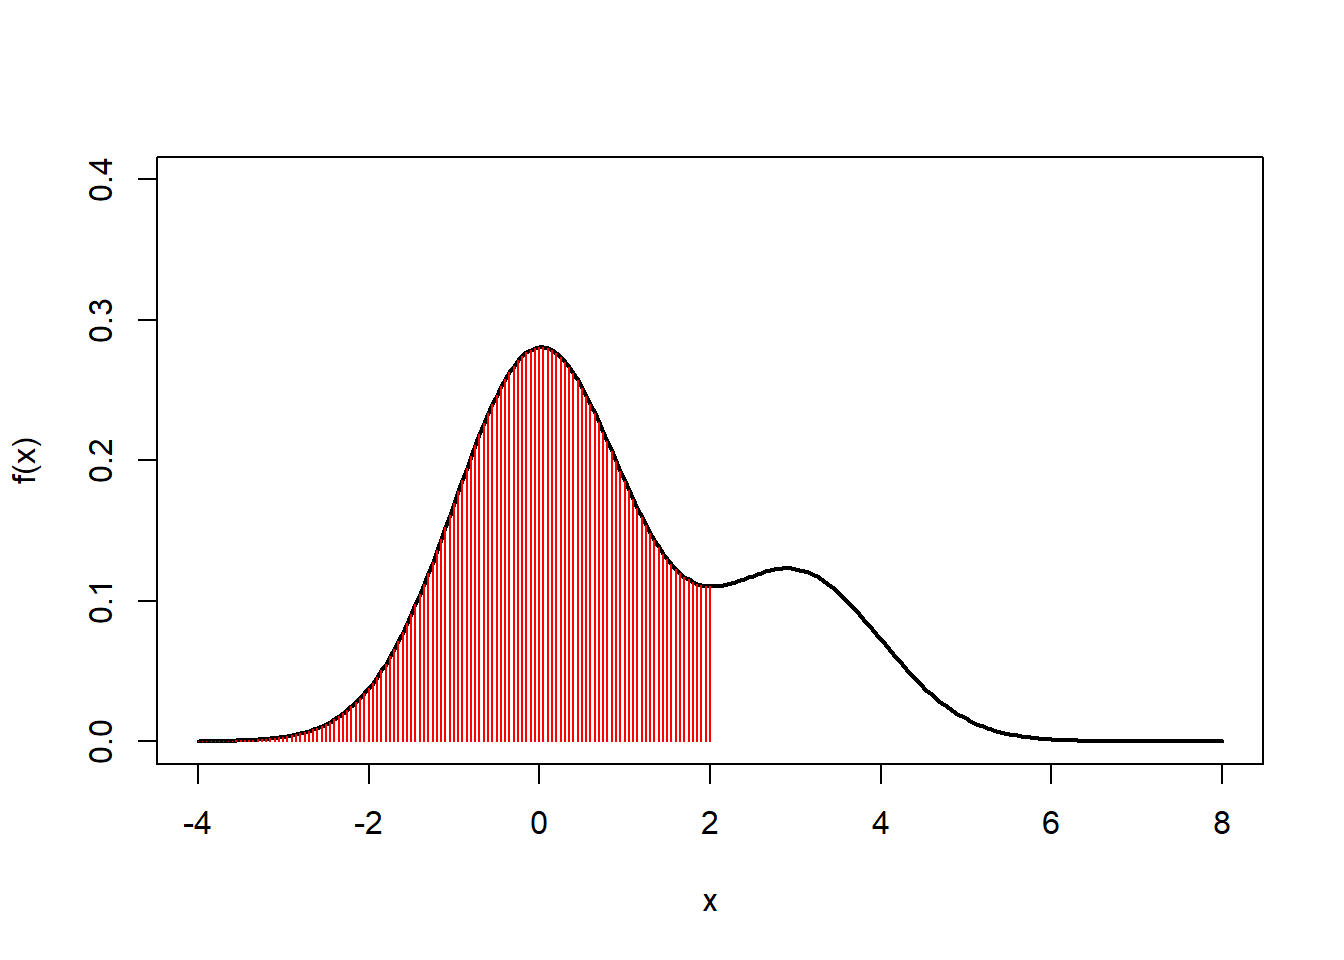
\includegraphics{_main_files/figure-latex/unnamed-chunk-45-1.pdf}

\begin{enumerate}
\def\labelenumi{\arabic{enumi})}
\setcounter{enumi}{1}
\tightlist
\item
  la probabilidad acumulada hasta \(a\) es
\end{enumerate}

\begin{itemize}
\tightlist
\item
  \(F(a) = P( X \leq a)\)
\end{itemize}

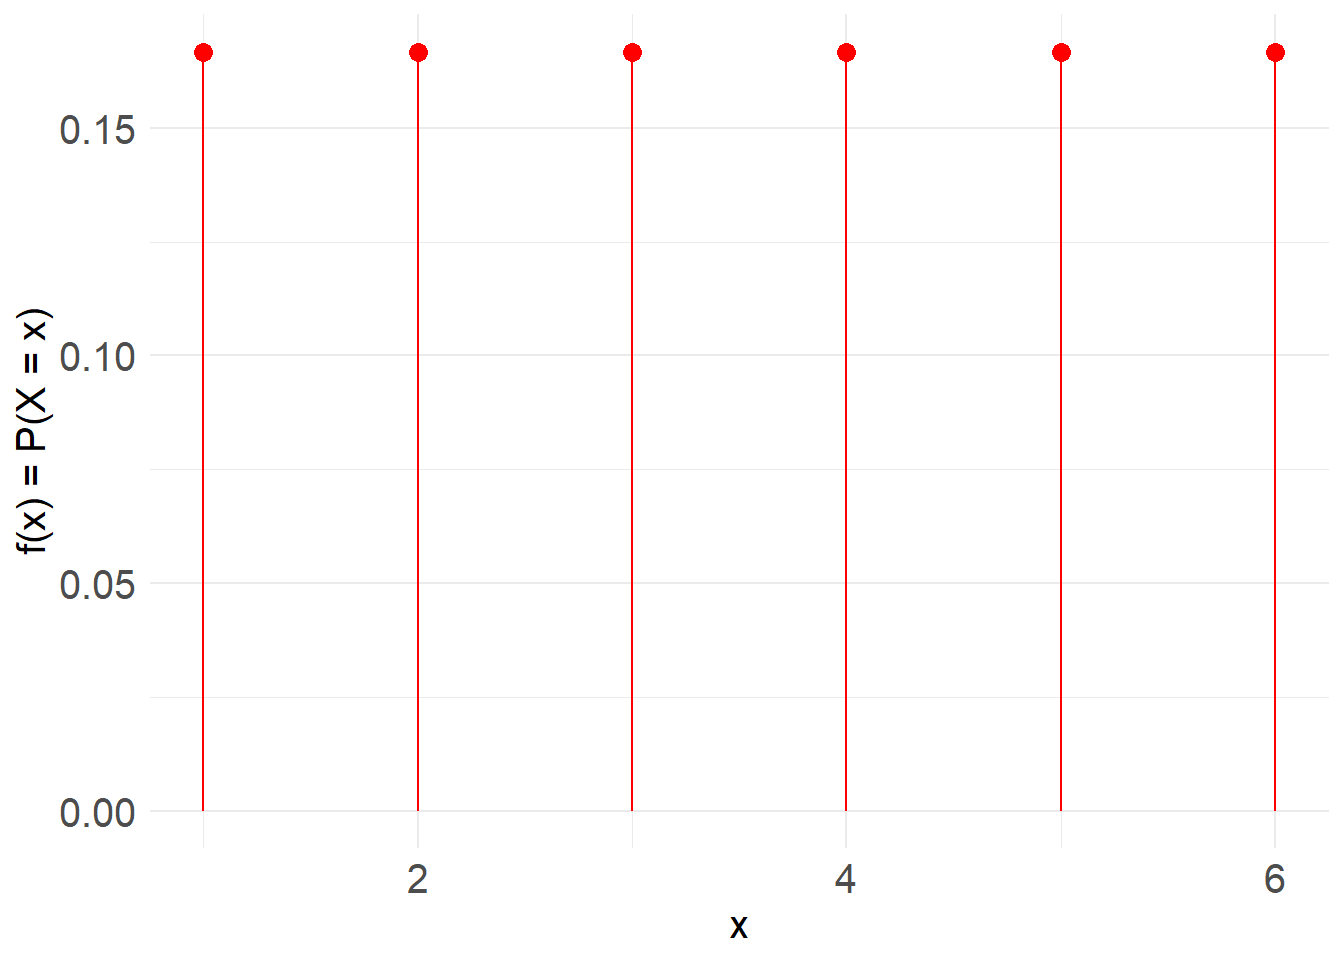
\includegraphics{_main_files/figure-latex/unnamed-chunk-46-1.pdf}

Entonces, la probabilidad entre \(a\) y \(b\) viene dada por la diferencia en el valor de la distribución de probabilidad

\begin{itemize}
\tightlist
\item
  \(P( a\leq X \leq b) = \int_a^b f(x)dx=F(b)-F(a)\)
\end{itemize}

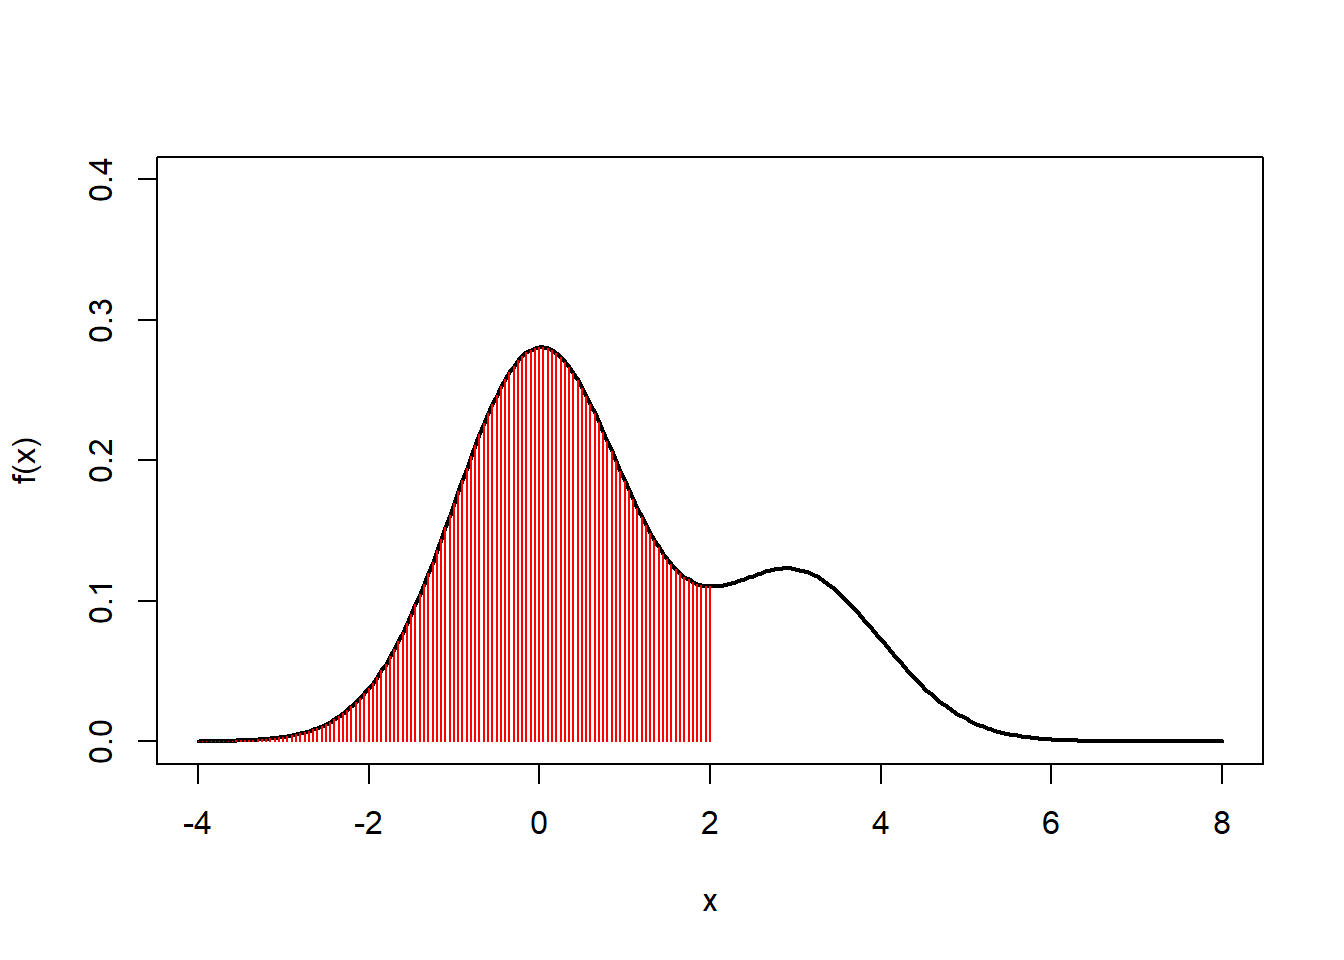
\includegraphics{_main_files/figure-latex/unnamed-chunk-47-1.pdf}

\textbf{Definición}

La \textbf{distribución de probabilidad} de una variable aleatoria continua se define como

\[F(a)= P( X\leq a) =\int_{-\infty } ^af(x)dx\]

y tiene las siguientes propiedades:

\begin{enumerate}
\def\labelenumi{\arabic{enumi})}
\tightlist
\item
  Está entre \(0\) y \(1\):
\end{enumerate}

\[F(-\infty )= 0\,\, y \,\,F(\infty )=1\]

\begin{enumerate}
\def\labelenumi{\arabic{enumi})}
\setcounter{enumi}{1}
\tightlist
\item
  Siempre aumenta:
\end{enumerate}

\[F(a)\leq F(b)\]

si \(a \leq b\)

\begin{enumerate}
\def\labelenumi{\arabic{enumi})}
\setcounter{enumi}{2}
\tightlist
\item
  Se puede utilizar para calcular probabilidades:
\end{enumerate}

\[P( a \leq X \leq b)=F(b)-F(a)\]

\begin{enumerate}
\def\labelenumi{\arabic{enumi})}
\setcounter{enumi}{3}
\tightlist
\item
  Recupera la densidad de probabilidad:
\end{enumerate}

\[f(x)=\frac{ dF (x )}{ dx}\]

Usamos \textbf{distribuciones de probabilidad} para \textbf{calcular probabilidades} de una variable aleatoria dentro de intervalos, y su derivada es la función de densidad de probabilidad.

\textbf{Ejemplo (gotas de lluvia)}

Para la función de densidad uniforme:

\[
    f(x)= 
\begin{cases}
    \frac{1}{100},& \text{si } x\in (0,100)\\
    0,& de\, otra\, forma 
\end{cases}
\]

Encontramos que la distribución de probabilidad es

\[
    F(a)= 
\begin{cases}
    0,& \text{si } a \leq 0 \\
    \frac{a}{100},& \text{si } a\in (0,100)\\
    1, & \text{si } 100 \leq a \\
    \\
\end{cases}
\]

\newpage

\hypertarget{gruxe1ficas-de-probabilidad}{%
\section{Gráficas de probabilidad}\label{gruxe1ficas-de-probabilidad}}

\begin{enumerate}
\def\labelenumi{\arabic{enumi})}
\tightlist
\item
  Podemos dibujar la probabilidad de una variable aleatoria en un intervalo como el \emph{área} bajo la curva de la \textbf{densidad}. Por ejemplo
\end{enumerate}

\[P(20<X< 60)\]

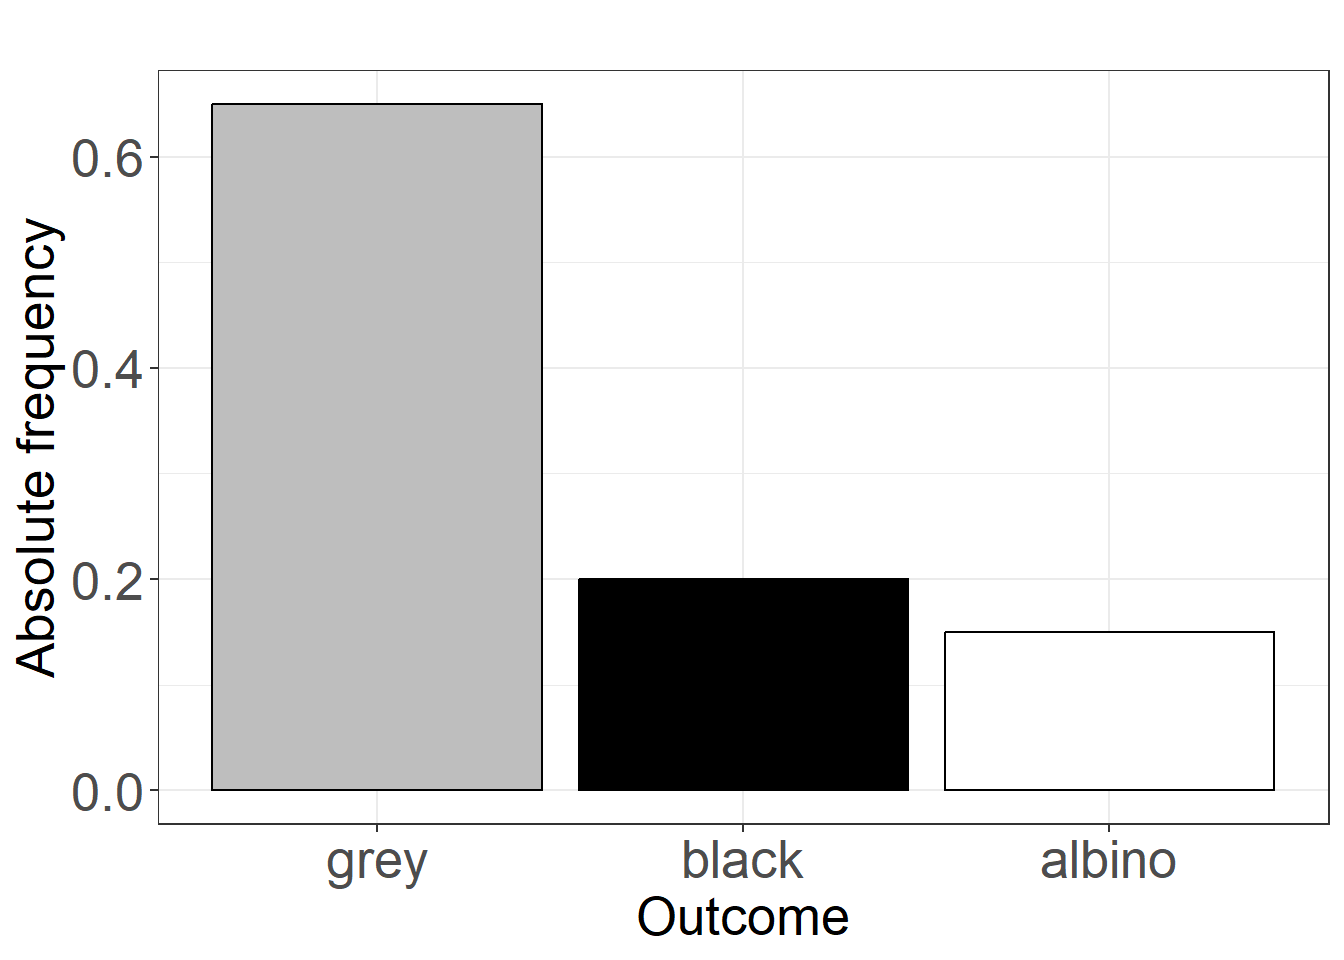
\includegraphics{_main_files/figure-latex/unnamed-chunk-48-1.pdf}

\begin{enumerate}
\def\labelenumi{\arabic{enumi})}
\setcounter{enumi}{1}
\tightlist
\item
  También podemos dibujar la probabilidad \(P(20<X< 60)\) como la \emph{diferencia} en los valores de la \textbf{distribución}
\end{enumerate}

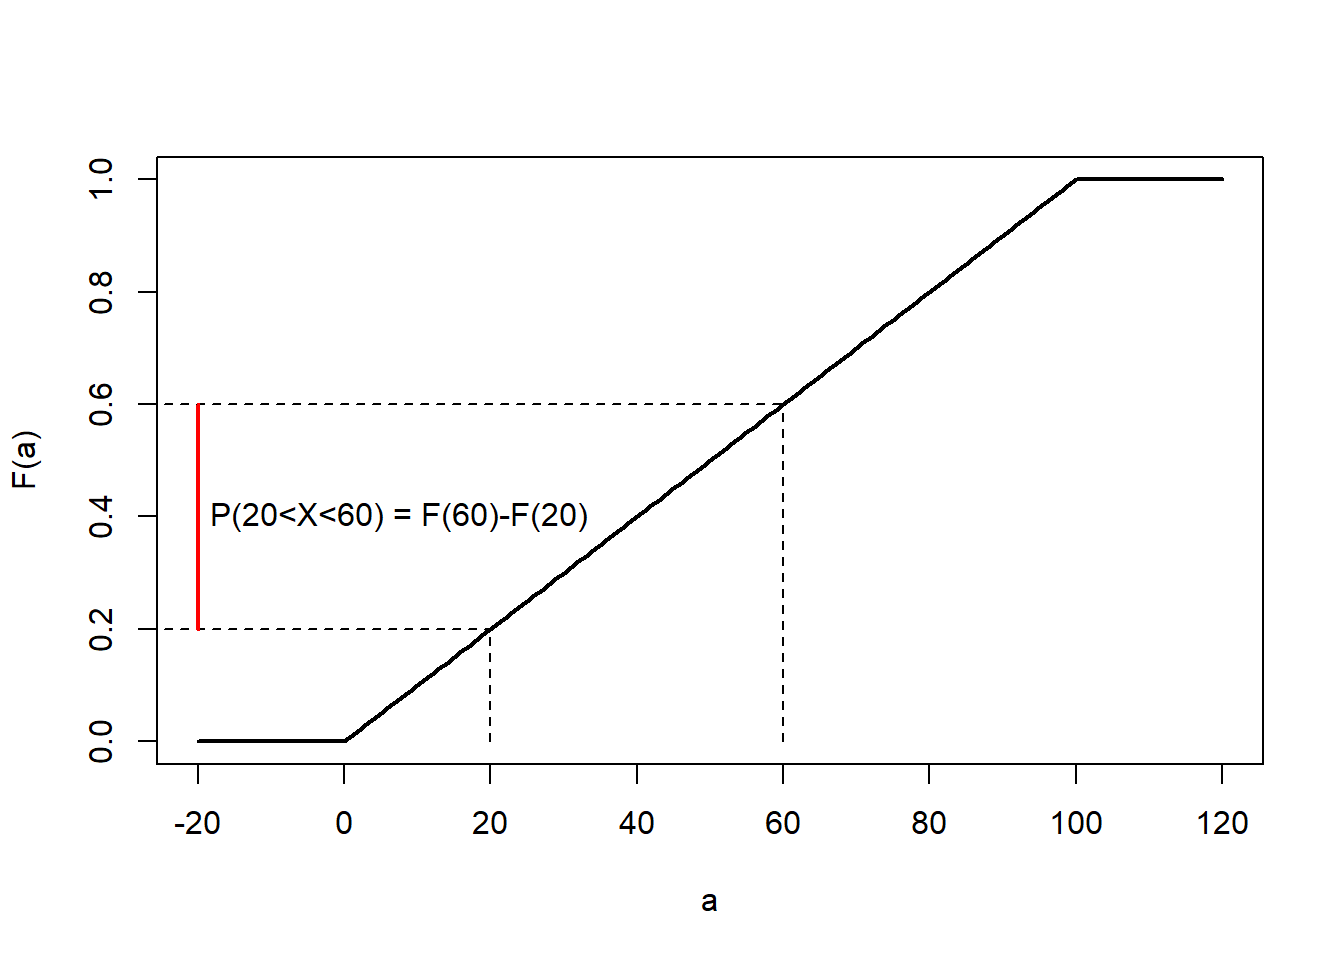
\includegraphics{_main_files/figure-latex/unnamed-chunk-49-1.pdf}

\hypertarget{media}{%
\section{Media}\label{media}}

Como en el caso discreto, la \textbf{media} mide el centro de masa de las probabilidades

\textbf{Definición}

Supongamos que \(X\) es una variable aleatoria continua con función de probabilidad \textbf{densidad} \(f(x)\). El valor medio o esperado de \(X\), denotado como \(\mu\) o \(E(X)\), es

\[\mu=E(X)=\int_{-\infty}^\infty x f(x) dx\]

Es la versión continua del centro de gravedad.

\textbf{Ejemplo (gotas de lluvia)}

La variable aleatoria con densidad de probabilidad

\[
    f(x)= 
\begin{cases}
    \frac{1}{100},& \text{si } x\in (0,100)\\
    0,& de\, otra\, forma 
\end{cases}
\]

Tiene un valor esperado en

\[E(X)=50\]

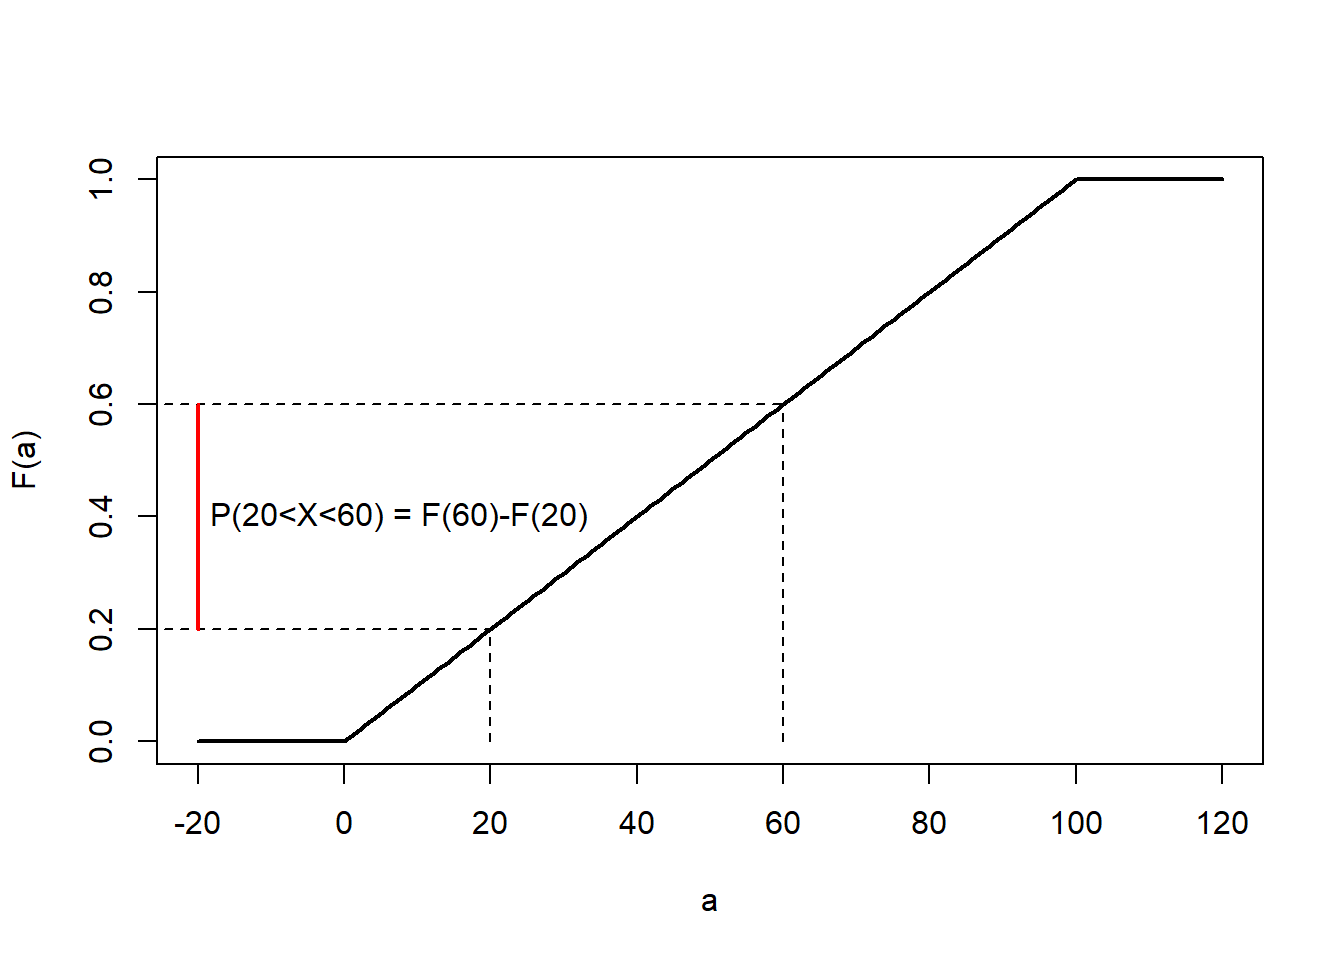
\includegraphics{_main_files/figure-latex/unnamed-chunk-50-1.pdf}

\hypertarget{varianza-1}{%
\section{Varianza}\label{varianza-1}}

Como en el caso discreto, la varianza mide la dispersión de probabilidades sobre la media

\textbf{Definición}

Supongamos que \(X\) es una variable aleatoria continua con función de densidad de probabilidad \(f(x)\). La varianza de \(X\), denotada como \(\sigma^2\) o \(V(X)\), es

\[\sigma^2=V(X)=\int_{-\infty}^\infty (x-\mu)^2 f(x) dx\]

Es la versión continua del momento de inercia.

\hypertarget{funciones-de-x}{%
\section{\texorpdfstring{Funciones de \(X\)}{Funciones de X}}\label{funciones-de-x}}

En muchas ocasiones, estaremos interesados en resultados que sean función de las variables aleatorias. Tal vez nos interese el cuadrado de la elongación de un muelle, o la raíz cuadrada de la temperatura de un motor.

\textbf{Definición}

Para cualquier función \(h\) de una variable aleatoria \(X\), con función de masa \(f(x)\), su valor esperado viene dado por

\[E[h(X)]= \int_{-\infty}^{\infty} h(x) f(x)dx\]
De esta definición recuperamos las mismas propiedades que en el caso discreto

\begin{enumerate}
\def\labelenumi{\arabic{enumi})}
\item
  La media de una función lineal es la función lineal de la media: \[ E( a\times X +b)= a\times E(X) +b\] para \(a\) y \(b\) escalares.
\item
  La varianza de una función lineal de \(X\) es:
\end{enumerate}

\[V(a\times X +b)= a^2\times V(X)\]

\begin{enumerate}
\def\labelenumi{\arabic{enumi})}
\setcounter{enumi}{2}
\tightlist
\item
  La varianza sobre el origen es la varianza sobre la media más la media al cuadrado:
\end{enumerate}

\[E(X^2)= V(X)+E(X)^2\]

\hypertarget{ejercicios-4}{%
\section{Ejercicios}\label{ejercicios-4}}

\hypertarget{ejercicio-1-3}{%
\subsubsection{Ejercicio 1}\label{ejercicio-1-3}}

Para la densidad de probabilidad

\[
    f(x)= 
\begin{cases}
    \frac{1}{100},& \text{si } x\in (0,100)\\
    0,& de\, otra\, forma 
\end{cases}
\]

\begin{itemize}
\tightlist
\item
  calcular la media (R:50)
\item
  calcular la varianza usando \(E(X^2)= V(X)+E(X)^2\) (R:100\^{}2/12)
\item
  calcula \(P( \mu-\sigma \leq X \leq \mu+\sigma)\) (R: 0.57)
\item
  ¿Cuáles son el primer y tercer cuartiles? (R: 25; 75)
\end{itemize}

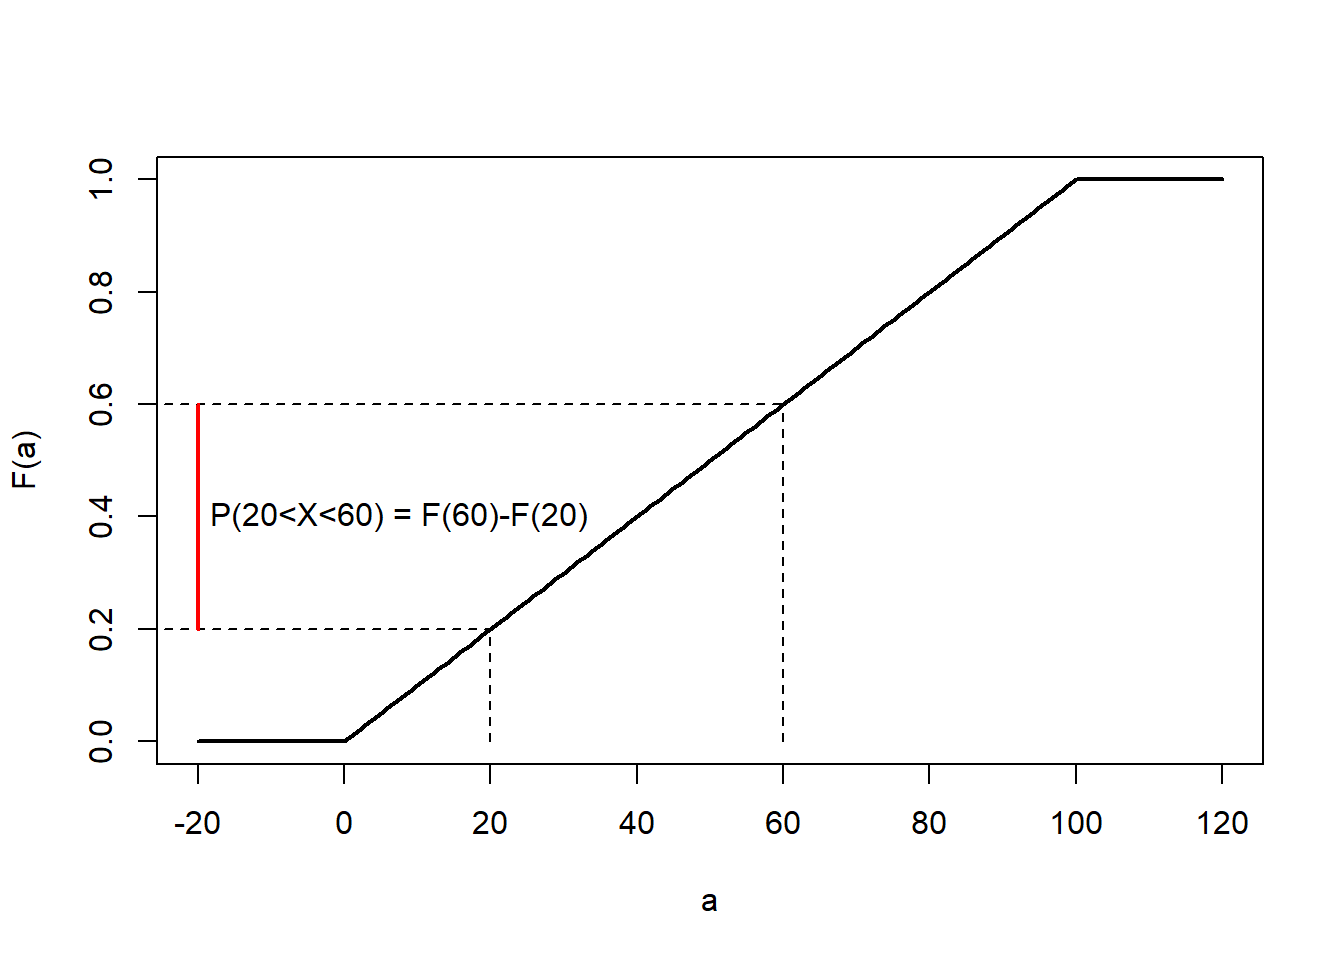
\includegraphics{_main_files/figure-latex/unnamed-chunk-51-1.pdf}

\hypertarget{ejercicio-2-3}{%
\subsubsection{Ejercicio 2}\label{ejercicio-2-3}}

Dado

\[
    f(x)= 
\begin{cases}
0, & x < 0 \\
ax, & x \in [0,3] \\
b, & x \in (3,5) \\
\frac{b}{3}(8-x),& x \in [5,8]\\
0, & x > 8 \\
\end{cases}
\]

\begin{itemize}
\item
  ¿Cuáles son los valores de \(a\) y \(b\) tales que \(f(x)\) es una función de densidad de probabilidad continua ? (R: 1/15; 1/5)
\item
  ¿Cuál es la media de \(X\)? (R:4)
\end{itemize}

\hypertarget{ejercicio-3-3}{%
\subsubsection{Ejercicio 3}\label{ejercicio-3-3}}

Para la densidad de probabilidad

\[
    f(x)= 
\begin{cases}
    \lambda e^{-\lambda x},& \text{si } x \geq 0\\
    0,& de\, otra\, forma 
\end{cases}
\]

\begin{itemize}
\tightlist
\item
  Confirmar que se trata de una densidad de probabilidad
\item
  Calcular la media (R: 1/\(\lambda\))
\item
  Calcule el valor esperado de \(X^2\) (R: 2/\(\lambda^2\))
\item
  Calcular la varianza (R: 1/\(\lambda^2\))
\item
  Hallar la distribución de probabilidad \(F(a)\) (R: \(1- exp( -\lambda a)\))
\item
  Encuentra la mediana (R: \(\log{ 2}\) /\(\lambda\))
\end{itemize}

\hypertarget{ejercicio-4-2}{%
\subsubsection{Ejercicio 4}\label{ejercicio-4-2}}

Dada la distribución acumulativa de una variable aleatoria \(X\)

\[
    F(x)= 
\begin{cases}
0, & x  < -1 \\
\frac{1}{80}(17+16x-x^2),& x \in [-1,7)\\
1,& x \geq 7\\
\end{cases}
\]

calcular:

\begin{itemize}
\tightlist
\item
  \(P(X> 0)\) (R:63/80)
\item
  \(E(X)\) (R:1.93)
\item
  \(P(X>0|X< 2)\) (R:28/45)
\end{itemize}

\hypertarget{modelos-de-probabilidad-para-variables-aletorias-discretas}{%
\chapter{Modelos de probabilidad para variables aletorias discretas}\label{modelos-de-probabilidad-para-variables-aletorias-discretas}}

\hypertarget{objetivo-3}{%
\section{Objetivo}\label{objetivo-3}}

En este capítulo veremos algunas funciones de masa de probabilidad que se utilizan para describir experimentos aleatorios comunes.

Introduciremos el concepto de parámetro y por tanto de modelos paramétricos.

En particular, discutiremos las funciones de probabilidad uniforme y de Bernoulli y cómo se usan para derivar las funciones de probabilidad binomial y binomial negativa. También hableramos del modelo hipergeométrico.

\hypertarget{funciuxf3n-de-probabilidad}{%
\section{Función de probabilidad}\label{funciuxf3n-de-probabilidad}}

Recordemos que una función de masa de probabilidad de una \textbf{variable aleatoria discreta} \(X\) con valores posibles \(x_1 , x_2 , .. , x_M\) es \textbf{cualquier función} tal que

\begin{enumerate}
\def\labelenumi{\arabic{enumi})}
\tightlist
\item
  Nos permite calcular probabilidades para todos los resultados
\end{enumerate}

\[f(x_i)=P(X=x_i)\]

\begin{enumerate}
\def\labelenumi{\arabic{enumi})}
\setcounter{enumi}{1}
\tightlist
\item
  Siempre es positiva:
\end{enumerate}

\[f(x_i)\geq 0\]

\begin{enumerate}
\def\labelenumi{\arabic{enumi})}
\setcounter{enumi}{2}
\tightlist
\item
  La probabilidad de obtener algo en el experimento aleatorio es \(1\)
\end{enumerate}

\[\sum_{i=1}^M f(x_i)=1\]

Estudiamos dos \textbf{propiedades importantes:}

\begin{enumerate}
\def\labelenumi{\arabic{enumi})}
\tightlist
\item
  La media como medida de tendencia central:
\end{enumerate}

\[E(X)= \sum_{i=1}^M x_i f(x_i)\]

\begin{enumerate}
\def\labelenumi{\arabic{enumi})}
\setcounter{enumi}{1}
\tightlist
\item
  La varianza como medida de dispersión:
\end{enumerate}

\[V(X)= \sum_{i=1}^M (x_i-\mu)^2 f(x_i)\]

\hypertarget{modelo-de-probabilidad}{%
\section{Modelo de probabilidad}\label{modelo-de-probabilidad}}

Un \textbf{modelo de probabilidad} es una función de masa de probabilidad que puede representar las probabilidades de un experimento aleatorio.

\textbf{Ejemplos:}

\begin{enumerate}
\def\labelenumi{\arabic{enumi})}
\tightlist
\item
  La función de masa de probabilidad definida por
\end{enumerate}

\begin{longtable}[]{@{}cc@{}}
\toprule\noalign{}
\(X\) & \(f(x)\) \\
\midrule\noalign{}
\endhead
\bottomrule\noalign{}
\endlastfoot
\(-2\) & \(1/8\) \\
\(-1\) & \(2/8\) \\
\(0\) & \(2/8\) \\
\(1\) & \(2/8\) \\
\(2\) & \(1/8\) \\
\end{longtable}

Representa la probabilidad de sacar \textbf{una} bola de una urna donde hay dos bolas con etiquetas: \(-1, 0, 1\) y una bola con etiquetas: \(-2, 2\).

\begin{enumerate}
\def\labelenumi{\arabic{enumi})}
\setcounter{enumi}{1}
\tightlist
\item
  \(f(x)=P(X=x)=1/6\) representa la probabilidad de los resultados de \textbf{un} lanzamiento de un dado.
\end{enumerate}

\hypertarget{modelos-paramuxe9tricos}{%
\section{Modelos paramétricos}\label{modelos-paramuxe9tricos}}

Cuando tenemos un experimento aleatorio con \(M\) resultados posibles, necesitamos encontrar \(M\) números para determinar la función de masa de probabilidad. Como en el ejemplo 1 anterior, necesitábamos \(5\) valores en la columna \(f(x)\) de la tabla de probabilidad.

Sin embargo, \textbf{en muchos casos}, podemos formular funciones de probabilidad \(f(x)\) que dependen únicamente de \textbf{muy pocos} números. Al igual que en el ejemplo 2 anterior, solo necesitábamos saber cuántos resultados posibles puede dar un dado.

\textbf{Ejemplo (probabilidad clásica):}

Un experimento aleatorio con \(M\) resultados igualmente probables tiene una función de masa de probabilidad:
\[f(x)=P(X=x)=1/M\]

Sólo necesitamos saber \(M\).

Los números que \textbf{necesitamos saber} para determinar completamente una función de probabilidad se llaman \textbf{parámetros}.

\hypertarget{distribuciuxf3n-uniforme-un-paruxe1metro}{%
\section{Distribución uniforme (un parámetro)}\label{distribuciuxf3n-uniforme-un-paruxe1metro}}

El ejemplo anterior es la interpretación clásica de la probabilidad y define nuestro primer modelo paramétrico.

\textbf{Definición}

Una variable aleatoria \(X\) con resultados \(\{1,...M\}\) tiene una \textbf{distribución uniforme} discreta si todos sus resultados \(M\) tienen la misma probabilidad

\[f(x)=\frac{1}{M}\]

\(M\) es el parámetro natural del modelo. Una vez que definimos \(M\) para un experimento, elegimos una función de masa de probabilidad particular. La función anterior es realmente una \textbf{familia} de funciones que dependen de \(M\): \(f(x; M)\).

La media y la varianza de una variable que sigue una distribución uniforme son:

\[E(X)= \frac{M+1}{2}\]

y

\[V(X)= \frac{M^2-1}{12}\]

Nota: \(E(X)\) y \(V(X)\) también son \textbf{parámetros}. Si conocemos alguno de ellos, entonces podemos determinar completamente la distribución. Por ejemplo:

\[f(x)=\frac{1}{2E(X)-1}\]

Veamos algunas funciones de masa de probabilidad en la familia de modelos paramétricos uniformes:

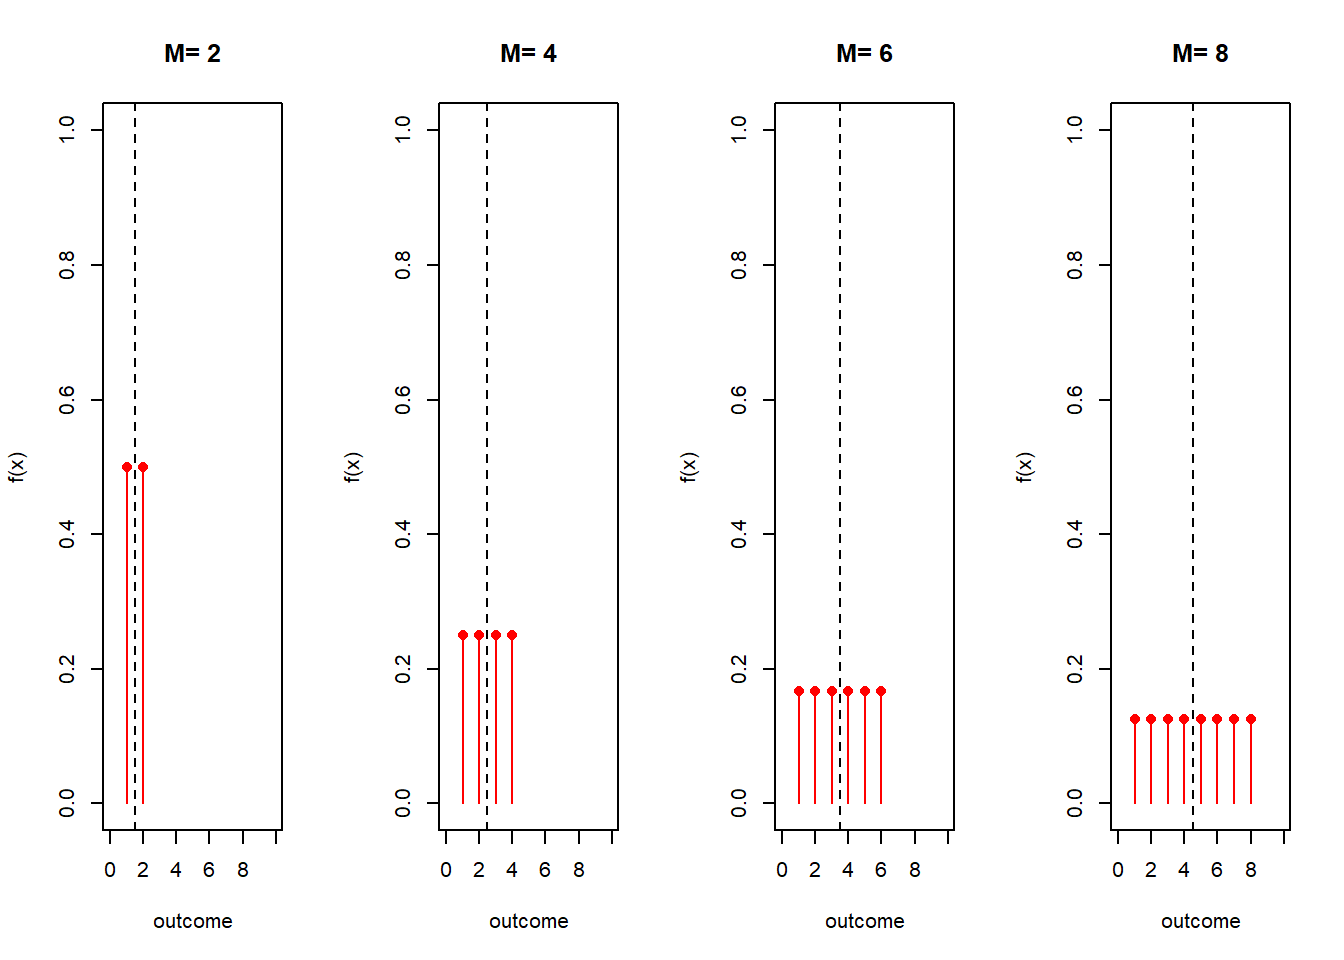
\includegraphics{_main_files/figure-latex/unnamed-chunk-52-1.pdf}

\hypertarget{distribuciuxf3n-uniforme-dos-paruxe1metros}{%
\section{Distribución uniforme (dos parámetros)}\label{distribuciuxf3n-uniforme-dos-paruxe1metros}}

Consideremos ahora un nuevo modelo de probabilidad \textbf{uniforme} con \textbf{dos parámetros}: los resultados mínimo y máximo.

Si la variable aleatoria toma valores en \(\{a, a+1, ...b\}\), donde \(a\) y \(b\) son números enteros y todos los resultados son igualmente probables, entonces

\[f(x)=\frac{1}{b-a+1}\]

porque \(M=b-a+1\).

Entonces decimos que \(X\) se distribuye uniformemente entre \(a\) y \(b\) y escribimos

\[X \rightarrow Unif(a,b)\]

\textbf{Propiedades:}

Si \(X\) se distribuye uniformemente entre \(a\) y \(b\)

\[X \rightarrow Unif(a,b)\]

\begin{enumerate}
\def\labelenumi{\arabic{enumi})}
\tightlist
\item
  Su media es
\end{enumerate}

\[E(X)= \frac{b+a}{2}\]

\begin{enumerate}
\def\labelenumi{\arabic{enumi})}
\setcounter{enumi}{1}
\tightlist
\item
  Su varianza es
\end{enumerate}

\[V(X)= \frac{(b-a+1)^2-1}{12}\]

Para probar esto cambia las variables \(X=Y+a-1\), \(y \in \{1,...M\}\).

\textbf{Funciones de masa de probabilidad}

Veamos algunas funciones de masa de probabilidad en la familia de modelos paramétricos uniformes:

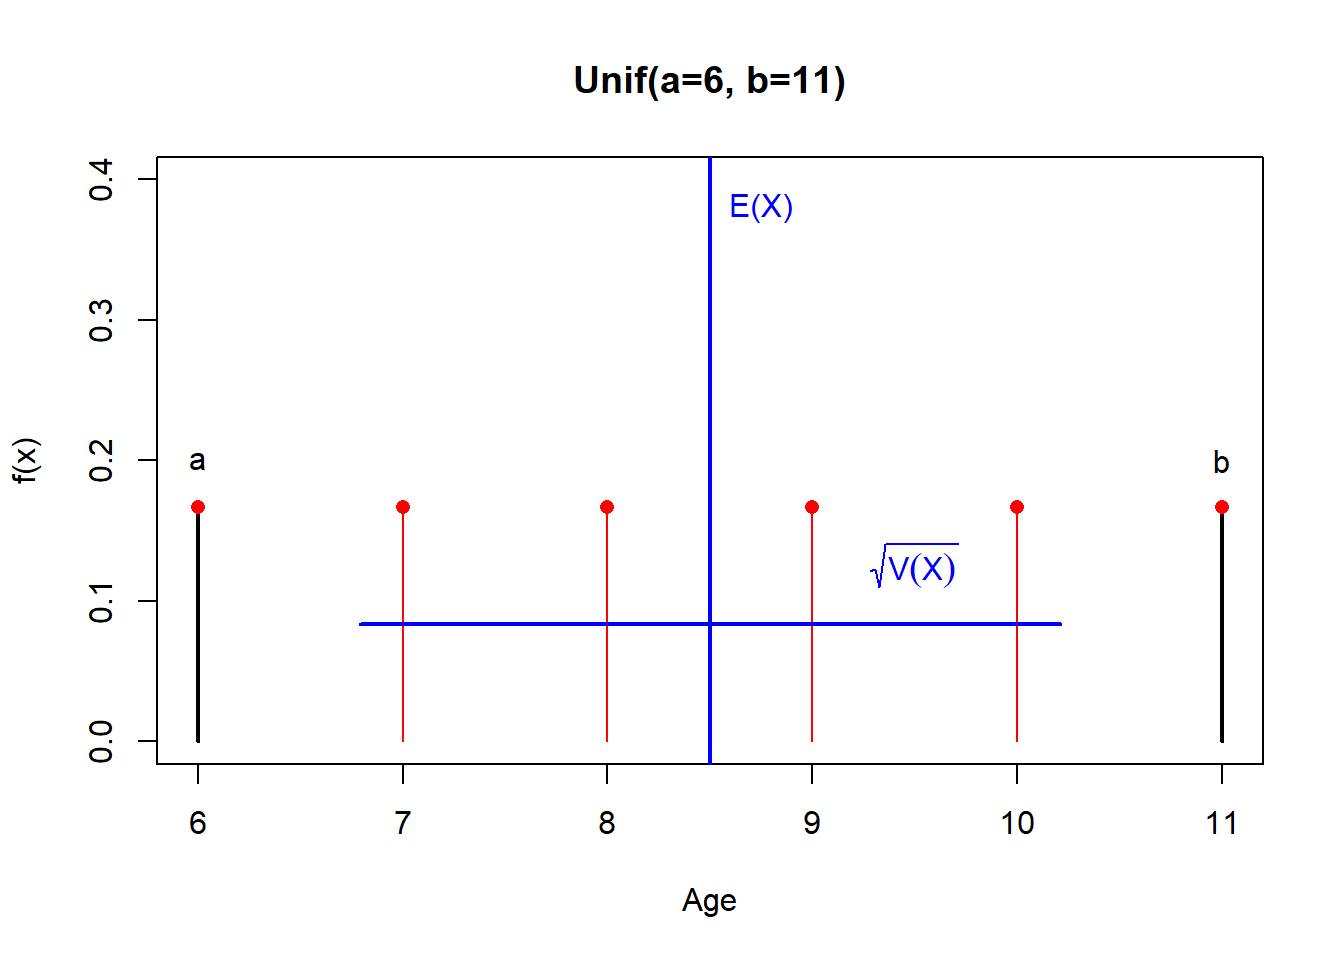
\includegraphics{_main_files/figure-latex/unnamed-chunk-53-1.pdf}

\textbf{Ejemplo (clases escolares):}

¿Cuál es la probabilidad de observar a un niño de una edad particular en una escuela primaria (si todas las clases tienen la misma cantidad de niños)?

Del diseño del experimento sabemos: \(a=6\) y \(b=11\) entonces

\[X \rightarrow Unif(a=6, b=11)\] eso es

\[f(x)=\frac{1}{6}\] para \(x\in \{6,7,8,9,10,11\}\), y \(0\) en caso contrario.

La media y la varianza de esta función de masa de probabilidad es:

\begin{itemize}
\tightlist
\item
  \(E(X)=8.5\)
\item
  \(V(X)=2.916667\)
\end{itemize}

Recuerda

\begin{itemize}
\item
  El valor esperado es la \textbf{media} \(\mu=8.5\)
\item
  La \textbf{desviación estándar} \(\sigma=1.707825\) es la distancia promedio desde la media y se calcula a partir de la raíz cuadrada de la varianza.
\end{itemize}

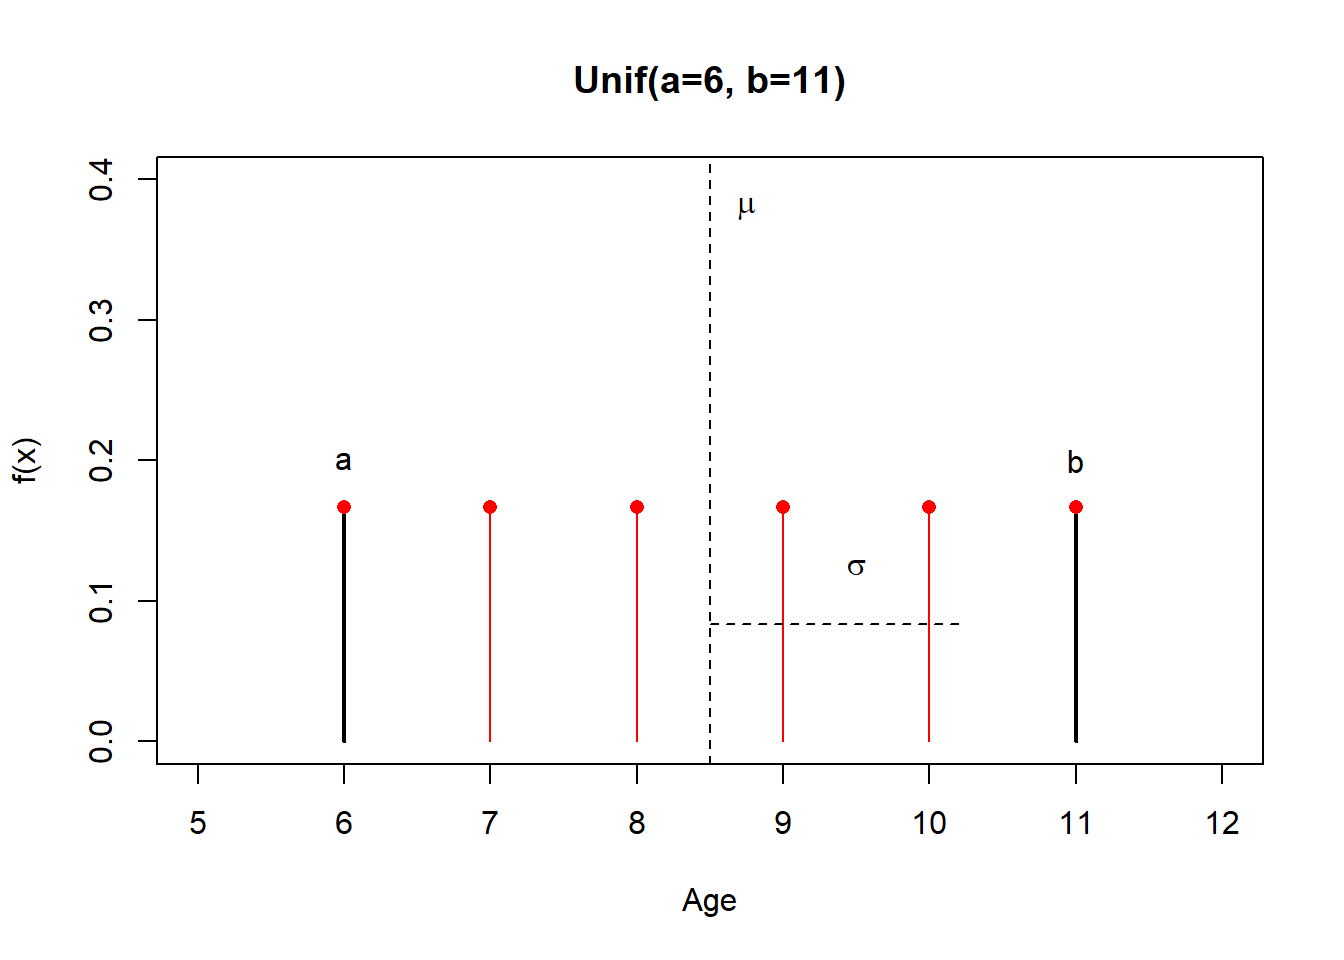
\includegraphics{_main_files/figure-latex/unnamed-chunk-54-1.pdf}

\textbf{Parámetros y Modelos:}

Un \textbf{modelo} es una función particular \(f(x)\) que \textbf{describe} nuestro experimento.

Si el modelo es una función \textbf{conocida} que depende de algunos parámetros, al cambiar el valor de los parámetros producimos una \textbf{familia de modelos}: \(f(x; a,b)\).

El conocimiento de \(f(x)\) se reduce al conocimiento del valor de los parámetros \(a\), \(b\).

Idealmente, el modelo y los parámetros son \textbf{interpretables}.

En nuestro ejemplo, \(a\) representa la edad mínima en la escuela y \(b\) la edad máxima. Pueden considerarse como las \textbf{propiedades físicas} del experimento.

\hypertarget{ensayo-de-bernoulli}{%
\section{Ensayo de Bernoulli}\label{ensayo-de-bernoulli}}

Ahora considermos un modelo con solo dos resultados posibles (\(A\) y \(B\)) que tienen probabilidades \textbf{desiguales}

\textbf{Ejemplos:}

\begin{itemize}
\item
  Anotar el sexo de un paciente que acude a urgencias de un hospital (\(A:masculino\) y \(B:femenino\)).
\item
  Registrar si una máquina fabricada es defectuosa o no (\(A:defectuosa\) y \(B:no\,\,defectuosa\)).
\item
  Dar en el blanco (\(A:éxito\) y \(B:fracaso\)).
\item
  Transmitir un píxel correctamente (\(A:sí\) y \(B:no\)).
\end{itemize}

En estos ejemplos, la probabilidad del resultado \(A\) suele ser \textbf{desconocida}.

\textbf{Modelo de probabilidad:}

Introduciremos la probabilidad de un resultado (\(A\)) como el \textbf{parámetro} del modelo. El modelo se puede escribir en diferentes formas.

\begin{enumerate}
\def\labelenumi{\arabic{enumi})}
\tightlist
\item
  Como una tabla de probabilidad:
\end{enumerate}

\begin{longtable}[]{@{}cc@{}}
\toprule\noalign{}
\(Resultado\) & \(P_i\) \\
\midrule\noalign{}
\endhead
\bottomrule\noalign{}
\endlastfoot
\(A\) & \(p\) \\
\(B\) & \(1-p\) \\
\end{longtable}

\begin{itemize}
\tightlist
\item
  \(i \in \{A,B\}\)
\item
  resultado \(A\) (éxito): tiene probabilidad \(p\) (parámetro)
\item
  resultado \(B\) (fracaso): tiene una probabilidad \(1-p\)
\end{itemize}

\begin{enumerate}
\def\labelenumi{\arabic{enumi})}
\setcounter{enumi}{1}
\tightlist
\item
  Como función de masa de probabilidad de la variable aleatoria \(K\) tomando valores \(\{0, 1\}\) para \(B\) y \(A\), respectivamente.
\end{enumerate}

\[
    f(k)= 
\begin{cases}
    1-p,&  k=0\, (event\, B)\\
    p,& k=1\, (event\, A) 
\end{cases}
\]

\begin{enumerate}
\def\labelenumi{\arabic{enumi})}
\setcounter{enumi}{2}
\tightlist
\item
  Como una función de \(k\)
\end{enumerate}

\[f(k; p)=p^k(1-p)^{1-k} \]

para \(k=(0,1)\).

Entonces decimos que \(K\) sigue una distribución de Bernoulli con parámetro \(p\)
\[K \rightarrow Bernoulli(p)\]

\textbf{Propiedades:}

Si \(K\) sigue una distribución de Bernoulli, entonces

\begin{enumerate}
\def\labelenumi{\arabic{enumi})}
\tightlist
\item
  su media es
\end{enumerate}

\[E(K)=p\]

\begin{enumerate}
\def\labelenumi{\arabic{enumi})}
\setcounter{enumi}{1}
\tightlist
\item
  su varianza es
\end{enumerate}

\[V(K)=(1-p)p\]

Ten en cuenta que la probabilidad del resultado \(A\) es el parámetro \(p\)
que es lo mismo que su valor en \(k=1\): \(f(1)=P(k=1)\). El parámetro determina completamente la función de masa de probabilidad, incluidas su media y varianza.

Veamos algunas funciones de masa de probabilidad en la familia de modelos paramétricos uniformes:

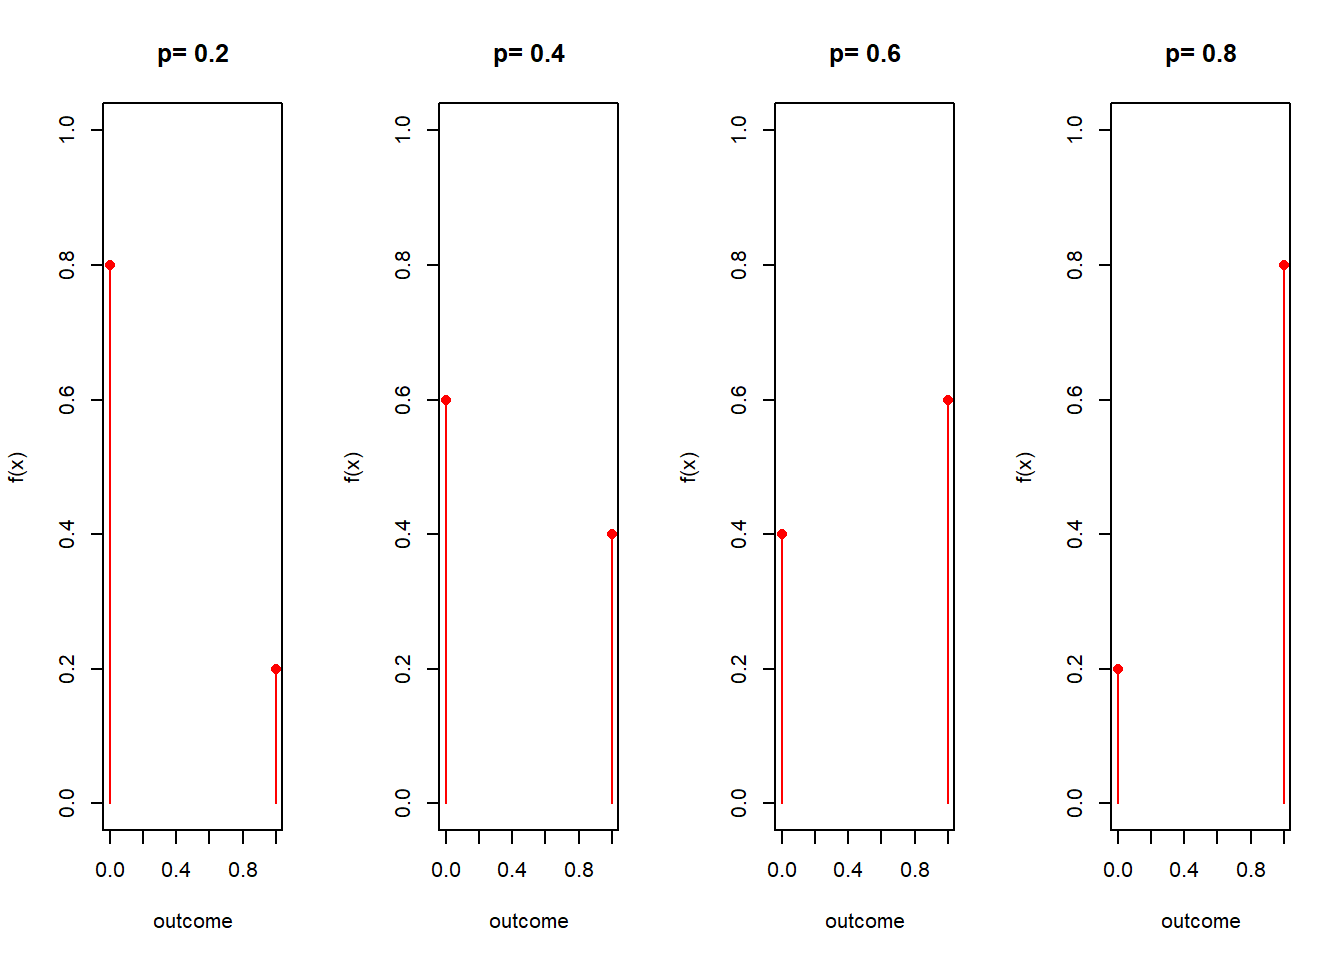
\includegraphics{_main_files/figure-latex/unnamed-chunk-55-1.pdf}

\hypertarget{experimento-binomial}{%
\section{Experimento binomial}\label{experimento-binomial}}

Si estamos interesados en predecir \textbf{frecuencias absolutas} cuando conocemos el parámetro \(p\) de un ensayo particular de Bernoulli, entonces

\begin{enumerate}
\def\labelenumi{\arabic{enumi})}
\item
  \textbf{repetimos} el ensayo de Bernoulli \(n\) veces y contamos cuantas veces obtuvimos \(A\); es decir, calculamos la frecuencia absoluta de \(A\): \(N_A\).
\item
  definimos una \textbf{variable aleatoria} \(X=N_A\) tomando valores \(x \in {0,1,...n}\)
\end{enumerate}

Cuando repetimos \(n\) veces una ensayo de Bernoulli, observamos un valor para \(n_A\). Si realizamos otros \(n\) ensayos de Bernoulli, entonces \(n_A\) cambia de valor. \(X=N_A\) es por lo tanto una variable aleatoria y \(X=n_A\) es su observación.

\textbf{Ejemplos (Algunos experimentos binomiales):}

\begin{itemize}
\item
  Anotamos el sexo de \(n=10\) pacientes que acuden a urgencias de un hospital. ¿Cuál es la probabilidad de que \(9\) (\(X=9\)) pacientes sean hombres cuando \(p=0.8\)?
\item
  Intentamos \(n=5\) veces de dar en un blanco (\(A:éxito\) y \(B:fracaso\)). ¿Cuál es la probabilidad de que alcancemos el objetivo \(5\) (\(X=5\)) veces cuando normalmente lo hacemos el \(25\%\) de las veces (\(p=0.25\))?
\item
  Transmitimos \(n=100\) píxeles correctamente (\(A:sí\) y \(B:no\)). ¿Cuál es la probabilidad de que \(2\) (\(X=2\)) píxeles sean errores, cuando la probabilidad de error es \(p=0.1\)?
\end{itemize}

\hypertarget{funciuxf3n-de-probabilidad-binomial}{%
\section{Función de probabilidad binomial}\label{funciuxf3n-de-probabilidad-binomial}}

Supongamos que \textbf{sabemos} el valor real del parámetro del ensayo de Bernoulli \(p\).

Cuando repetimos un ensayo de Bernoulli y paramos en la repetición número \(n\), ¿el valor \(x\) que obtenemos es un valor común o es raro? ¿cuál es su función de masa de probabilidad \(P(X=x)=f(x)\)?

\textbf{Ejemplo (transmisión de píxeles):}

¿Cuál es la probabilidad de observar errores \(X=x\) al transmitir \(n=4\) píxeles, si la probabilidad de error es \(p\)?

Consideremos que

\begin{enumerate}
\def\labelenumi{\arabic{enumi})}
\item
  Una variable aleatoria del \textbf{experimento de transmisión} es el vector \[(K_1, K_2, K_3, K_4)\] donde una observación puede ser \((K_1=0, K_2=1, K_3=0, K_4= 1)\) o \((0, 1, 0, 1)\).
\item
  Cada \[K_i \rightarrow Bernoulli(p)\] \(k_i \in \{0, 1\}\)
\item
  \(X=N_A\) se puede calcular como la suma \[X=\sum_{i=1}^4 K_i\] \(x\in \{0,1,2,3,4\}\). Por ejemplo \(X=2\) para el resultado \((0, 1, 0, 1)\).
\end{enumerate}

Ahora veamos las probabilidades del número de \textbf{errores} y luego las generalizaremos.

\begin{enumerate}
\def\labelenumi{\arabic{enumi})}
\tightlist
\item
  ¿Cuál es la probabilidad de observar \(4\) \textbf{errores} (\(X=4\))?
\end{enumerate}

La probabilidad de observar \(4\) errores es la probabilidad de observar un error en \(1^{er}\) \textbf{y} \(2^{o}\) \textbf{y} \(3^{o}\) \textbf{y} \(4 ^{o}\) píxel:

\[P(X=4)=P(1,1,1,1)=p*p*p*p=p^4\]

porque \(K_i\) son \textbf{independientes}.

\begin{enumerate}
\def\labelenumi{\arabic{enumi})}
\setcounter{enumi}{1}
\tightlist
\item
  ¿Cuál es la probabilidad de observar \(0\) \textbf{errores} (\(X=0\))?
\end{enumerate}

La probabilidad de errores \(0\) es la probabilidad conjunta de observar \textbf{ningún error} en \textbf{cualquier} transmisión:

\[P(X=0)=P(0,0,0,0)=(1-p)(1-p)(1-p)(1-p)=(1-p)^4\]

\begin{enumerate}
\def\labelenumi{\arabic{enumi})}
\setcounter{enumi}{2}
\tightlist
\item
  ¿Cuál es la probabilidad de observar \(3\) \textbf{errores}?
\end{enumerate}

La probabilidad de \(3\) errores es la \textbf{suma} de la probabilidad de observar \(3\) errores en \textbf{eventos diferentes}:

\[P(X=3)=P(0,1,1,1)+P(1,0,1,1)+P(1,1,0,1)+P(1,1,1, 0)=4p^3(1-p)^1\]
porque todos estos eventos son \textbf{mutuamente excluyentes}.

\begin{enumerate}
\def\labelenumi{\arabic{enumi})}
\setcounter{enumi}{3}
\tightlist
\item
  Por lo tanto, la probabilidad de \(x\) \textbf{errores} es
\end{enumerate}

\[
    f(x)= 
\begin{cases}
    1*p^0(1-p)^4,&  x=0 \\
    4*p^1(1-p)^3,&  x=1 \\
    6*p^2(1-p)^2,&  x=2 \\
    4*p^3(1-p)^1,&  x=3 \\
    1*p^4(1-p)^0,&  x=4 \\
\end{cases}
\]

o más en breve

\[f(x)=\binom 4 xp^x(1-p)^{4-x}\]
para \(x=0,1,2,3,4\)

donde \(\binom 4 x\) es el número de \textbf{posibles resultados} (transmisiones de \(4\) píxeles) con \(x\) errores.

\textbf{Definición:}

La función de \textbf{probabilidad binomial} es la función de masa de probabilidad de observar \(x\) resultados de tipo \(A\) en \(n\) ensayos independientes de Bernoulli, donde \(A\) tiene la misma probabilidad \(p\) en cada ensayo.

La función está dada por

\(f(x)=\binom nxp^x(1-p)^{nx}\), \(x=0,1,...n\)

\(\binom nx= \frac{n!}{x!(nx)!}\) se denomina \textbf{coeficiente binomial} y da el número de formas en que se pueden obtener \(x\) eventos de tipo \(A\) en un conjunto de \(n\).

Cuando una variable \(X\) tiene una función de probabilidad binomial decimos que se distribuye binomialmente y escribimos

\[X\rightarrow Bin(n,p)\]

donde \(n\) y \(p\) son parámetros.

Veamos algunas funciones de masa de probabilidad en la familia de modelos paramétricos binomiales:

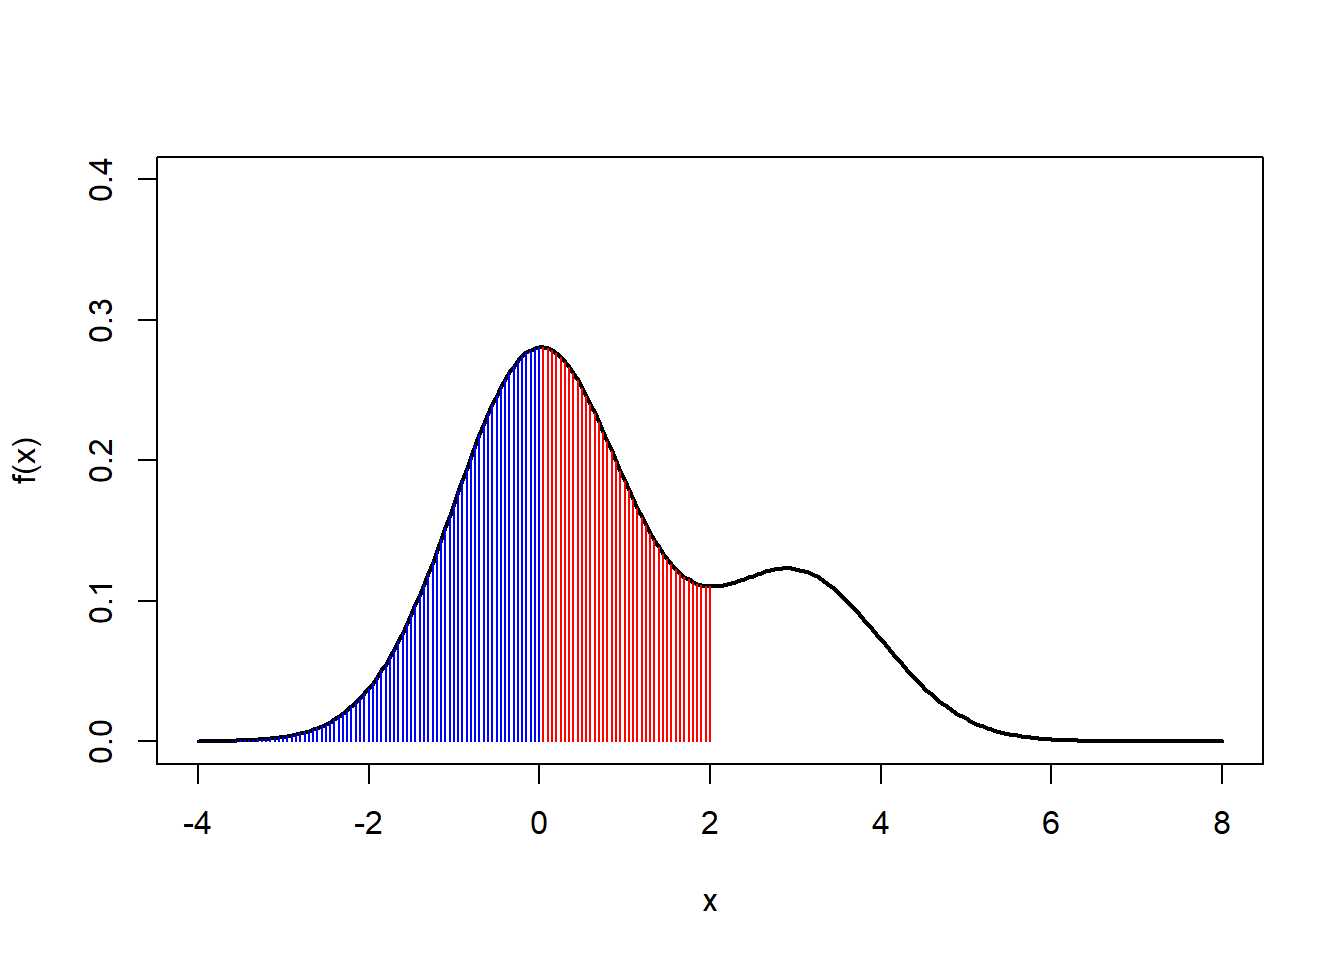
\includegraphics{_main_files/figure-latex/unnamed-chunk-56-1.pdf}

\textbf{Propiedades:}

Si una variable aleatoria \(X\rightarrow Bin(n,p)\) entonces

\begin{enumerate}
\def\labelenumi{\arabic{enumi})}
\tightlist
\item
  su media es
\end{enumerate}

\[E(X)=np\]

\begin{enumerate}
\def\labelenumi{\arabic{enumi})}
\setcounter{enumi}{1}
\tightlist
\item
  su varianza es
\end{enumerate}

\[V(X)=np(1-p)\]

Estas propiedades se pueden demostrar por el hecho de que \(X\) es la suma de \(n\) variables de Bernoulli independientes. Por lo tanto,

\(E(X)=E(\sum_{i=1}^n K_i)=np\)

y

\(V(X)=V(\sum_{i=1}^n K_i)=n(1-p)p\)

\textbf{Ejemplo (transmisión de píxeles):}

\begin{itemize}
\item
  El valor esperado para el número de errores en la transmisión de \(4\) píxeles es \(np=4*0.1=0.4\) cuando la probabilidad de error es \(0.1\).
\item
  La varianza es \(n(1-p)p=0.36\)
\item
  ¿Cuál es la probabilidad de observar \(4\) errores?
\end{itemize}

Dado que estamos repitiendo una ensayo de Bernoulli \(n=4\) veces y contando el número de eventos de tipo \(A\) (errores), cuando \(P(A)=p=0.1\) entonces

\[X \rightarrow Bin(n=4, p=0.1)\]
Eso es \[f(x)=\binom 4 x 0.1^x(1-0.1)^{4-x}\]

\(P(X=4)=f(4)=\binom 4 4 0.1^4 0.9^{0}=0.1^4=10^{-4}\)

En R dbinom(4,4,0.1)

\begin{itemize}
\tightlist
\item
  ¿Cuál es la probabilidad de observar \(2\) errores?
\end{itemize}

\(P(X=2)=\binom 4 2 0.1^2 0.9^2=0.0486\)

En R dbinom(2,4,0.1)

\textbf{Ejemplo (encuestas de opinión):}

\begin{itemize}
\tightlist
\item
  ¿Cuál es la probabilidad de observar \textbf{como máximo} \(8\) votantes del partido de gobierno en una encuesta electoral de tamaño \(10\), si la probabilidad de un voto para el partido es de \(0.9\)?
\end{itemize}

Para este caso

\[X \rightarrow Bin(n=10, p=0.9)\]

Eso es \[f(x)=\binom {10} x 0.9^x(0.1)^{4-x}\]

Queremos calcular:
\(P(X\le 8)=F(8)= \sum_{i=1..8} f(x_i)=0.2639011\)

en R pbinom(8,10, 0.9)

\hypertarget{funciuxf3n-de-probabilidad-binomial-negativa}{%
\section{Función de probabilidad binomial negativa}\label{funciuxf3n-de-probabilidad-binomial-negativa}}

Ahora imaginemos que estamos interesados en contar los píxeles bien transmitidos antes de que ocurra un \textbf{número dado} de errores. Digamos que podemos \textbf{tolerar} \(r\) errores en la transmisión.

Nuestro experimento aleatorio ahora es: Repetir las pruebas de Bernoulli hasta que observemos que el resultado \(A\) aparece \(r\) veces.

El resultado del experimento es el número de eventos \(B\) es decir \(n_B=y\).

Estamos interesados en encontrar la probabilidad de observar un número particular de eventos \(B\), \(P(Y=y)\), donde \(Y=N_B\) es la variable aleatoria.

\textbf{Ejemplo (transmisión de píxeles):}

¿Cuál es la probabilidad de observar \(y\) píxeles bien transmitidos (\(B\)) antes de \(r\) errores (\(A\))?

Primero encontremos la probabilidad de \textbf{un} evento de transmisión \textbf{en particular} con \(y\) número de píxeles correctos (\(B\)) y \(r\) número de errores (\(A\)).

\[(0,0,1,., 0,1,...0,1)\]

donde consideramos que hay \(y\) ceros y \(r\) unos. Por lo tanto, observamos \(y\) píxeles correctos en un total de \(y + r\) píxeles.

La probabilidad de este evento es:

\[P(0,0,1,., 0,1,...0,1)=p^r(1-p)^y\]

Recuerda que \(p\) es la probabilidad de error (\(A\)).

¿Cuántos \textbf{eventos de transmisión} pueden tener \(y\) píxeles correctos (0) antes de \(r\) errores (1)?

Ten en cuenta que

\begin{enumerate}
\def\labelenumi{\arabic{enumi})}
\item
  El último pixel es fijo (marca el final de la transmisión)
\item
  El número total de formas en que \(y\) el número de ceros se puede asignar en \(y + r-1\) píxeles es: \(\binom {y + r-1} y\)
\end{enumerate}

Por lo tanto, la probabilidad de observar \(y\) 1 antes de \(r\) 0 (cada 1 con probabilidad \(p\)) es

\[P(Y=y)=f(y)=\binom {y+r-1} yp^r(1-p)^y\]

para \(y=0,1,...\)

Entonces decimos que \(Y\) sigue una distribución binomial negativa y escribimos

\[Y\rightarrow NB(r,p)\]

donde \(r\) y \(p\) son parámetros que representan la tolerancia y la probabilidad de un solo error (evento \(A\)).

\textbf{Propiedades:}

Una variable aleatoria \(Y\rightarrow NB(r,p)\) tiene

\begin{enumerate}
\def\labelenumi{\arabic{enumi})}
\item
  media \[E(Y)= r\frac{1-p}{p}\]
\item
  y varianza \[V(Y)= r\frac{1-p}{p^2}\]
\end{enumerate}

Veamos algunas funciones de masa de probabilidad en la familia de modelos paramétricos binomiales negativos:

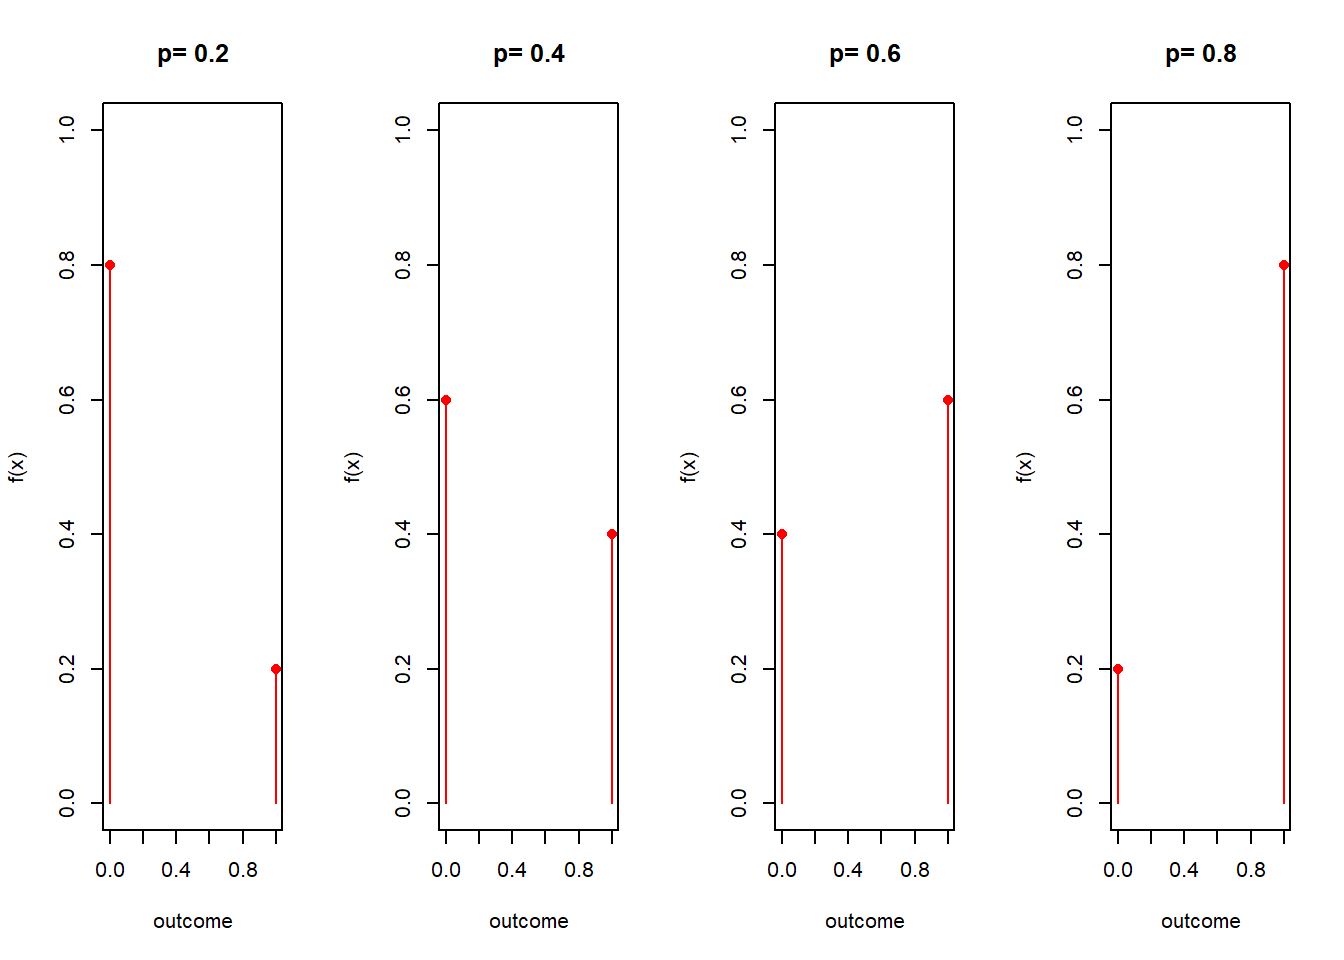
\includegraphics{_main_files/figure-latex/unnamed-chunk-57-1.pdf}

\textbf{Ejemplo (sitio web)}

Un sitio web tiene tres servidores. Un servidor opera a la vez y solo cuando falla una solicitud se usa otro servidor.

Si se sabe que la probabilidad de que falle una solicitud es \(p=0.0005\), entonces

\begin{itemize}
\tightlist
\item
  ¿Cuál es el número esperado de solicitudes exitosas antes de que las tres computadoras fallen?
\end{itemize}

Ya que estamos repitiendo un ensayo de Bernoulli hasta \(r=3\) se observan eventos de tipo \(A\) (fallo) (cada uno con \(P(A)=p=0.0005\)) y estamos contando el número de eventos de tipo \(B\) (solicitudes exitosas) entonces

\[Y \rightarrow NB(r=3, p=0.0005)\]

Por lo tanto, el número esperado de solicitudes antes de que el sistema falle es:

\(E(Y)=r\frac{1-p}{p}=3\frac{1-0.0005}{0.0005}=5997\)

Ten en cuenta que en realidad hay pruebas de \(6000\).

\begin{itemize}
\tightlist
\item
  ¿Cuál es la probabilidad de observar \(5\) solicitudes exitosas antes de que el sistema falle?
\end{itemize}

\(f(5)=\binom {7} 5 0.0005^3 0.9995^5=2.618444 \times 10^{-9}\)

\begin{itemize}
\tightlist
\item
  ¿Cuál es la probabilidad de tratar con un máximo de \(5\) solicitudes exitosas antes de que el sistema falle?
\end{itemize}

En R esto se calcula con dnbinom(5,3,0.0005)

Por lo tanto, queremos calcular la distribución de probabilidad en \(5\):

\(F(5)=P(Y\leq 5)=\Sigma_{y=0}^5 f(y)\)

\(=\sum_{y=0}^5\binom {y+2} y 0.0005^r0.9995^y\)

\(=\binom{2} 0 0.0005^3 0.9995^0 +\binom{3} 1 0.0005^3 0.9995^1\)

\(+\binom {4} 2 0.0005^3 0.9995^2 +\binom {5} 3 0.0005^3 0.9995^3\)

\(+\binom {6} 4 0.0005^3 0.9995^4 +\binom {7} 5 0.0005^3 0.9995^5\)

\(= 6.9\times 10^{-9}\)

En R esto se calcula con pnbinom(5,3,0.0005)

\textbf{Ejemplos}

\begin{itemize}
\tightlist
\item
  ¿Cuál es la probabilidad de observar \(10\) píxeles correctos antes de \(2\) errores, si la probabilidad de error es \(0.1\)?
\end{itemize}

\(f(10; r=2, p=0.1)=0.03835463\)

en R dnbinom(10, 2, 0.1)

\begin{itemize}
\tightlist
\item
  ¿Cuál es la probabilidad de que entren \(2\) chicas antes que \(4\) chicos entren a clase si la probabilidad de que entre un chico es de \(0.55\)?
\end{itemize}

\(f(2; r=4, p=0.55)=0.1853\)

en R dnbinom(2, 4, 0.55)

\hypertarget{distribuciuxf3n-geomuxe9trica}{%
\section{Distribución geométrica}\label{distribuciuxf3n-geomuxe9trica}}

Llamamos \textbf{distribución geométrica} a la distribución \textbf{binomial negativa} con \(r=1\)

La probabilidad de observar \(B\) eventos antes de observar el \textbf{primer} evento de tipo \(A\) es

\[P(Y=y)=f(y)= p(1-p)^y\]

\[Y\rightarrow Geom(p)\]
que tiene

\begin{enumerate}
\def\labelenumi{\arabic{enumi})}
\item
  media \[E(Y)= \frac{1-p}{p}\]
\item
  y varianza \[V(Y)= \frac{1-p}{p^2}\]
\end{enumerate}

\hypertarget{modelo-hipergeomuxe9trico}{%
\section{Modelo hipergeométrico}\label{modelo-hipergeomuxe9trico}}

El \textbf{modelo hipergeométrico} surge cuando queremos contar el número de eventos de tipo \(A\) que se extraen de una población finita.

El modelo general es considerar \(N\) bolas totales en una urna. Marquemos \(K\) con la etiqueta \(A\) y \(NK\) con la etiqueta \(B\). Saquemos \(n\) bolas una por una sin reemplazo en la urna y luego contemos cuántos \(A\) obtuvimos.

El modelo \textbf{Binomial} se puede derivar del modelo \textbf{Hipergeométrico} cuando consideramos que \(N\) es infinito, o que cada vez que sacamos una bola la volvemos a colocar en la urna.

\textbf{Ejemplo (varicela):}

Una escuela de \(N=600\) niños tiene una epidemia de varicela. Testamos a \(n=200\) niños y observamos que \(x=17\) dieron positivo. Si supiéramos que un total de \(K=64\) estaban realmente infectados en la escuela, ¿cuál es la probabilidad de nuestra observación?

\textbf{Definición:}

La probabilidad de obtener \(x\) casos (tipo \(A\)) en una muestra de \(n\) extraída de una población de \(N\) donde \(K\) son casos (tipo \(A\)).

\(P(X=x)=P(una\,muestra) \times (Número\, de\, formas\, de\, obteniendo\, x)\)

\[=\frac{1}{\binom N n}\binom K x \binom {NK} {nx}\]

donde \(k \in \{\max(0, n+KN), ... \min(K, n) \}\)

Entonces decimos que \(X\) sigue una distribución hipergeométrica y escribimos

\[X \rightarrow Hipergeom(N,K,n)\]
El modelo hipergeométrico tiene tres parámetros.

\textbf{Propiedades:}

Si \(X \rightarrow Hypergeometric(N,K,n)\) entonces tiene

\begin{enumerate}
\def\labelenumi{\arabic{enumi})}
\item
  media \[E(X) = n \frac{K}{N} = np\]
\item
  y varianza \[V(X) = np(1-p)\frac{Nn}{N-1}\]
\end{enumerate}

cuando \(p=\frac{K}{N}\) es la proporción de casos (\(A\)) en una población de tamaño \(N\). Ten en cuenta que cuando \(N \rightarrow \infty\) recuperamos las propiedades binomiales.

Veamos algunas funciones de masa de probabilidad en la familia de modelos paramétricos hipergeométricos:

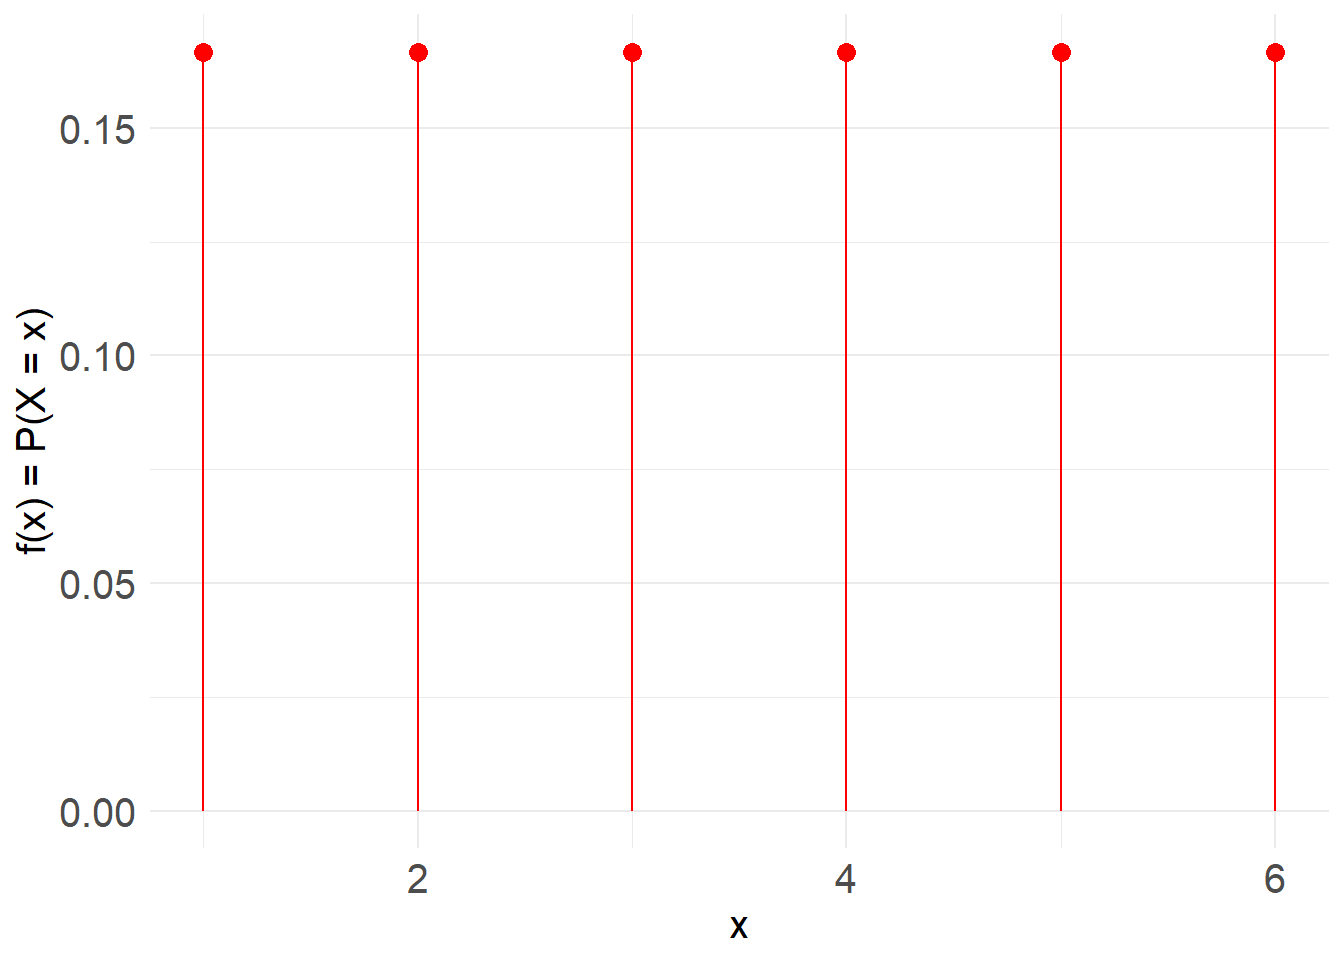
\includegraphics{_main_files/figure-latex/unnamed-chunk-58-1.pdf}

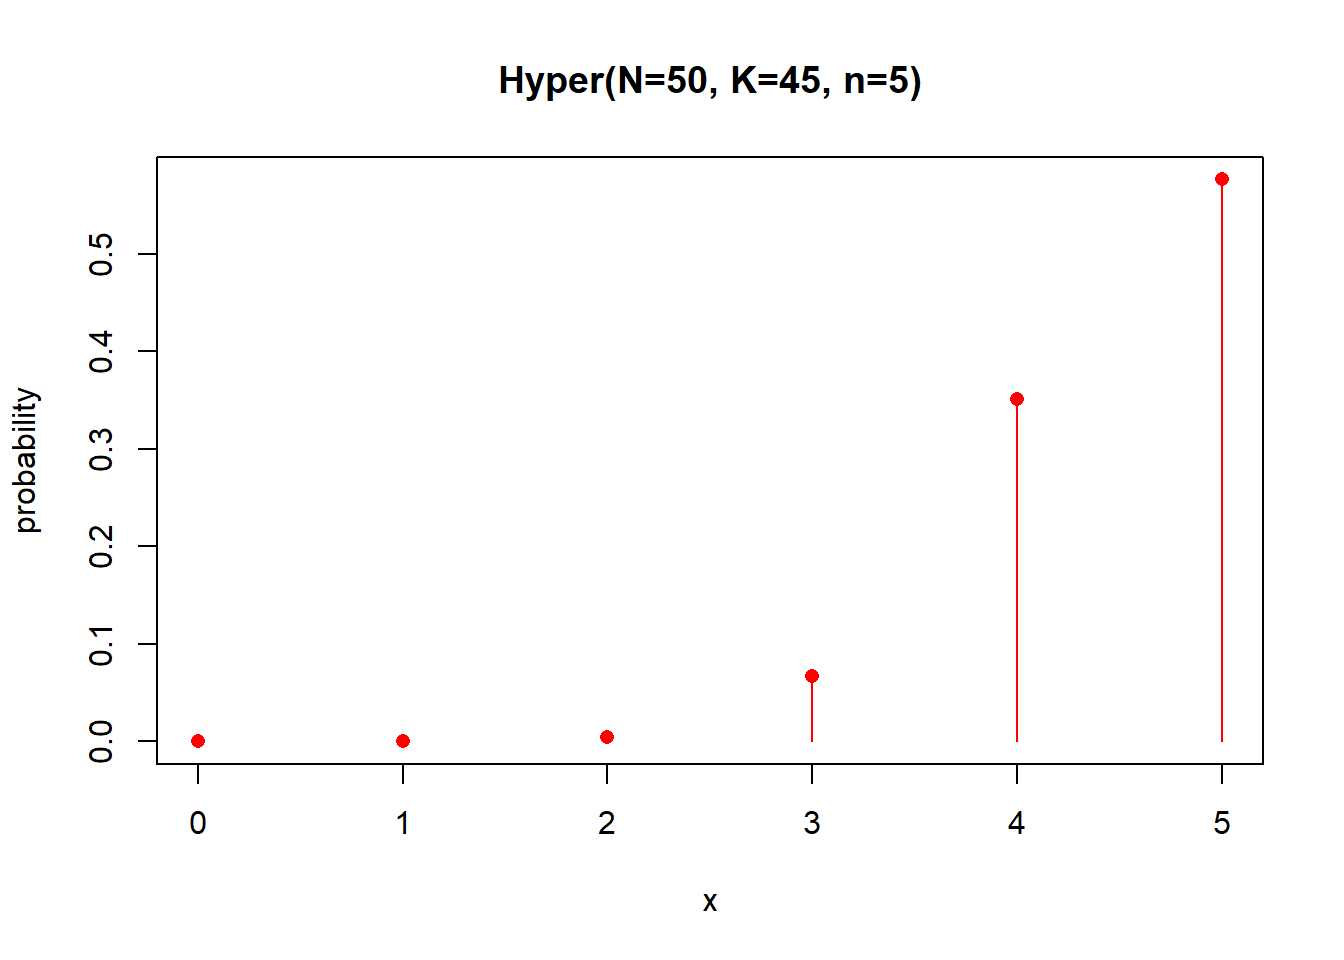
\includegraphics{_main_files/figure-latex/unnamed-chunk-59-1.pdf}

\textbf{Ejemplo (varicela):}

\begin{itemize}
\tightlist
\item
  ¿Cuál es la probabilidad ver como mucho \(17\) casos de varicela en una muestra de \(200\) alumnos de una ecuela de \(600\) alumnos donde \(64\) están infectados?
\end{itemize}

La probabilidad que necesitamos calcular es
\(P(X \leq 17)=F(17)\)

donde \(X \rightarrow Hypergeometric(N=600,K=64,n=200)\)

en R phyper(17, 64, 600-64, 200)=0.140565

La solución es la adición de las agujas azules en el gráfico.

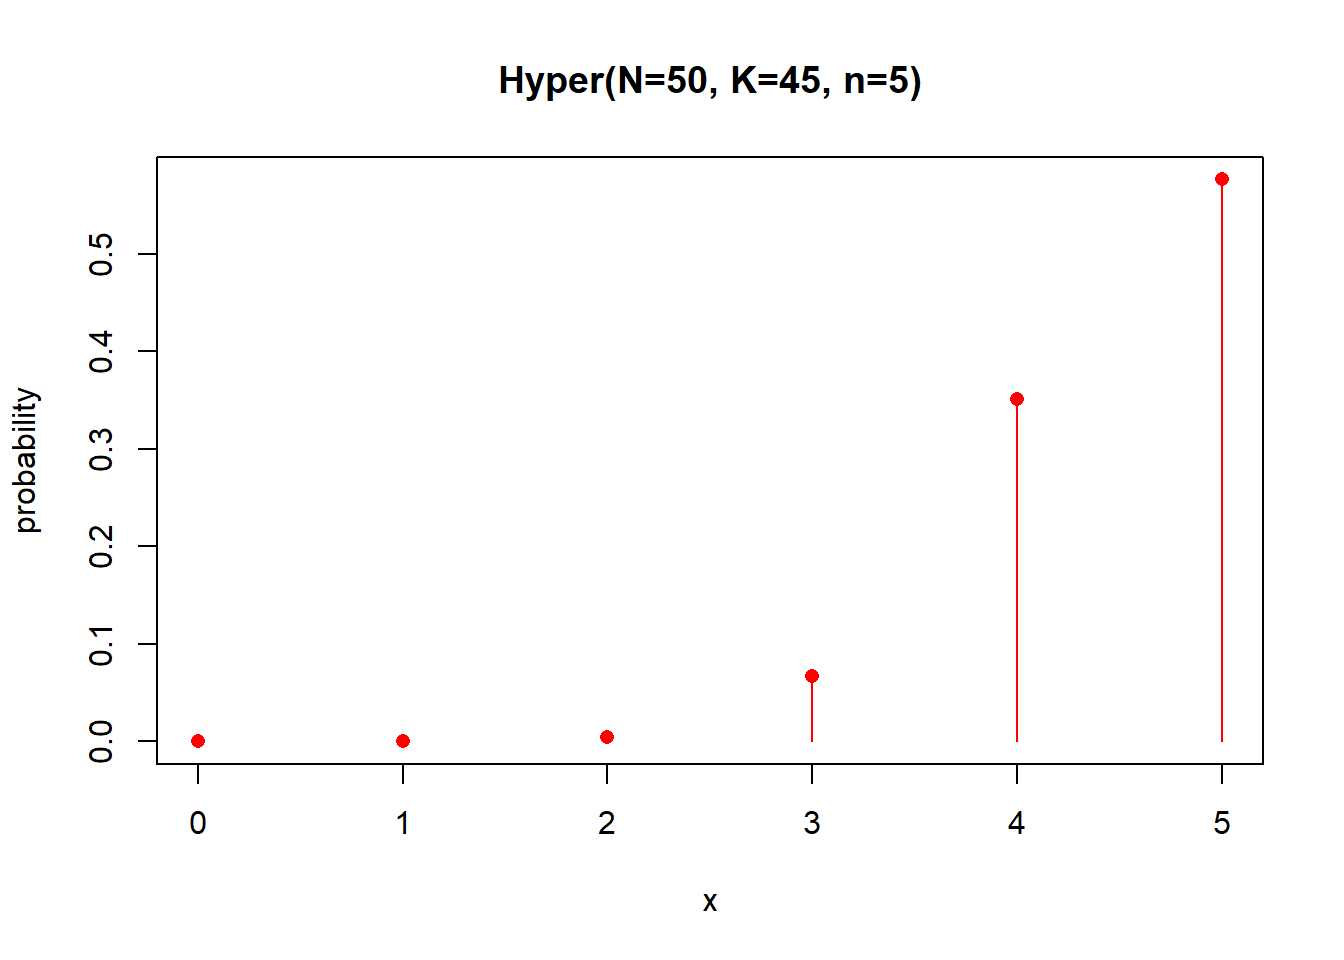
\includegraphics{_main_files/figure-latex/unnamed-chunk-60-1.pdf}

\hypertarget{preguntas-4}{%
\section{Preguntas}\label{preguntas-4}}

\textbf{1)} ¿Cuál es el valor esperado y la varianza del número de fallos en \(100\) prototipos, cuando la probabilidad de un fallo es de \(0.25\)?

\textbf{\(\qquad\)a:} \(0.25\), \(0.1875\);
\textbf{\(\qquad\)b:} \(25\), \(0.1875\);
\textbf{\(\qquad\)c:} \(0.25\), \(18.75\);
\textbf{\(\qquad\)d:} \(25\), \(18.75\)

\textbf{2)} ¿Qué modelo de probabilidad describe mejor el número de mesas disponibles a la hora de la cena en un restaurante?

\textbf{\(\qquad\)a:} Binomial;
\textbf{\(\qquad\)b:} Uniforme;
\textbf{\(\qquad\)c:} Binomial negativo;
\textbf{\(\qquad\)d:} Hipergeométrico

\textbf{3)} El valor esperado de una distribución Binomial no es

\textbf{\(\qquad\)a:} \(n\) veces el valor esperado de un Bernoulli;
\textbf{\(\qquad\)b:} el valor esperado de un Hipergeométrico, cuando la población es muy grande;
\textbf{\(\qquad\)c:} \(np\);
\textbf{\(\qquad\)d:} el límite de la frecuencia relativa cuando el número de repeticiones es grande

\textbf{4)} Las encuestas de opinión para las elecciones de EE. UU. dan una probabilidad de \(0.55\) de que un votante esté a favor del partido republicano. Si realizamos nuestra propia encuesta y preguntamos a 100 personas al azar en la calle, ¿cómo calcularías la probabilidad de que en nuestra encuesta los demócratas ganen las elecciones?

\textbf{\(\qquad\)a:}pbinom(x=49, n=100, p=0.55)=0.13;
\textbf{\(\qquad\)b:}1-pbinom(x=49, n=100, p=0.55)=0.86;
\textbf{\(\qquad\)c:}pbinom(x=51, n=100, p=0.45)=0.90; \textbf{\(\qquad\)d:}1-pbinom(x=51, n=100, p=0.45)=0.095

\textbf{5)} En un examen un alumno cuando no sabe la respuesta elige al azar una de las cuatro respuestas en una pregunta de selección múltiple. Si no sabe \(10\) preguntas, ¿cuál es la probabilidad de que al mas de \(5\) preguntas (\(>5\)) sean correctas?

\textbf{\(\qquad\)a:}dbinom(x=4, n=10, p=0.25); \textbf{\(\qquad\)b:}pbinom(x=4, n=10, p=0.75); \textbf{\(\qquad\)c:}dbinom(x=4, n=10, p=0.75); \textbf{\(\qquad\)d:}1-pbinom(x=4, n=10, p=0.25)

\hypertarget{ejercicios-5}{%
\section{Ejercicios}\label{ejercicios-5}}

\hypertarget{ejercicio-1-4}{%
\subsubsection{Ejercicio 1}\label{ejercicio-1-4}}

Si el 25\% de los tornillo producidos por una máquina son defectuosos, determina la probabilidad de que, de
5 tornillos elegidos al azar

\begin{itemize}
\tightlist
\item
  ningún tornillo sea defectuoso (R:0.2373)
\item
  1 tornillo sea defectuoso (R:0.3955)
\item
  2 tornillos sean defectuosos (R:0.2636)
\item
  como máximo 2 tornillos sean defectuosos (R:0.8964)
\end{itemize}

\hypertarget{ejercicio-2-4}{%
\subsubsection{Ejercicio 2}\label{ejercicio-2-4}}

En una población, la probabilidad de que nazca un niño es \(p=0.51\). Considera una familia de 4 hijos.

\begin{itemize}
\tightlist
\item
  ¿Cuál es la probabilidad de que una familia tenga un solo niño? (R: 0.240)
\item
  ¿Cuál es la probabilidad de que una familia tenga una sola niña? (R: 0.259)
\item
  ¿Cuál es la probabilidad de que una familia tenga solo un niño o solo una niña? (R: 0.4999)
\item
  ¿Cuál es la probabilidad de que la familia tenga por mucho dos niños? (R: 0.6723)
\item
  ¿Cuál es la probabilidad de que la familia tenga al menos dos niños? (R: 0.7023)
\item
  ¿Cuál es el mínimo número de hijos que debe tener una familia para que la probabilidad de tener al menos una niña sea mayor a \(0.75\)?(R:\(n=3 \geq\log(0.25)/\log(0.51)=2.05\))
\end{itemize}

\hypertarget{ejercicio-3-4}{%
\subsubsection{Ejercicio 3}\label{ejercicio-3-4}}

Un motor de búsqueda falla al recuperar información con una probabilidad de \(0.1\)

\begin{itemize}
\item
  Si nuestro sistema recibe \(50\) solicitudes de búsqueda, ¿cuál es la probabilidad de que el sistema no responda a tres de ellas? (R: 0.1385651)
\item
  ¿Cuál es la probabilidad de que el motor complete con éxito \(15\) búsquedas antes del primer fallo? (R:0.020)
\item
  Consideramos que un motor de búsqueda funciona suficientemente bien cuando es capaz de encontrar información como mínimo para \(10\) solicitudes por cada \(2\) fallos. ¿Cuál es la probabilidad de que en un ensayo de fiabilidad nuestro buscador sea satisfactorio? (R: 0.659)
\end{itemize}

\hypertarget{modelos-de-poisson-y-exponencial}{%
\chapter{Modelos de Poisson y Exponencial}\label{modelos-de-poisson-y-exponencial}}

\hypertarget{objetivo-4}{%
\section{Objetivo}\label{objetivo-4}}

En este capítulo veremos dos modelos de probabilidad estrechamente relacionados: los modelos \textbf{Poisson} y \textbf{exponencial}.

El modelo de Poisson es para variables aleatorias discretas, mientras que la función exponencial es para variables aleatorias \textbf{continuas}

\hypertarget{modelos-de-probabilidad-para-variables-discretas}{%
\section{Modelos de probabilidad para variables discretas}\label{modelos-de-probabilidad-para-variables-discretas}}

En el capítulo anterior construimos modelos complejos a partir de modelos simples. En cada etapa, introdujimos algún concepto novedoso:

\textbf{Uniforme}: interpretación clásica de la probabilidad
\(\downarrow\)
\textbf{Bernoulli}: Introducción de un \textbf{parámetro} \(p\) (familia de modelos)
\(\downarrow\)
\textbf{Binomial}: Introducción a la \textbf{Repetición} de un experimento aleatorio (\(n\) ensayos de Bernoulli)
\(\downarrow\)
\textbf{Poisson}: Repetición de un experimento aleatorio dentro de un intervalo continuo, sin \textbf{control} sobre cuándo/dónde ocurre el ensayo de Bernoulli.

El último modelo es para procesos de Poisson que describen la repetición de un experimento aleatorio con la aleatoriedad adicional del momento en que la repeticiones se producen.

\hypertarget{experimento-de-poissson}{%
\section{Experimento de Poissson}\label{experimento-de-poissson}}

Imagina que estamos observando eventos que \textbf{dependen} de \textbf{intervalos} de tiempo o distancia.

Por ejemplo:

\begin{itemize}
\tightlist
\item
  coches que llegan a un semáforo
\item
  mensajes que recibimos en el teléfono móvil
\item
  impurezas que ocurren al azar en un alambre de cobre
\end{itemize}

Supongamos que los eventos son resultados de ensayos de Bernoulli \textbf{independientes}, cada uno de los cuales aparece aleatoriamente en un intervalo continuo, y queremos \textbf{contarlos}.

¿Cuál es la probabilidad de observar \(X\) eventos en una unidad de intervalo (tiempo o distancia)?

\textbf{Ejemplo (Impurezas en un alambre):}

Imaginemos que algunas impurezas se depositan al azar a lo largo de un cable de cobre. Quieremos contar el número de impurezas en un centímetro de alambre (\(X\)).

Considera que sabemos que en promedio hay \(10\) impurezas por centímetro \(\lambda=10/cm\).

¿Cuál es la probabilidad de observar \(X=5\) impurezas en una muestra de un centímetro en particular?

\hypertarget{funciuxf3n-de-masa-de-probabilidad-de-poisson}{%
\section{Función de masa de probabilidad de Poisson}\label{funciuxf3n-de-masa-de-probabilidad-de-poisson}}

Para calcular la función masa de probabilidad \(f(x)=P(X=x)\) del ejemplo anterior dividimos el centímetro en micrómetros (\(0.0001cm\)).

Los micrómetros son lo suficientemente pequeños como para

\begin{enumerate}
\def\labelenumi{\arabic{enumi})}
\item
  que hay ao no haya una impureza en cada micrómetro
\item
  cada micrómetro se pueda considerar como un \textbf{ensayo de Bernoulli}
\end{enumerate}

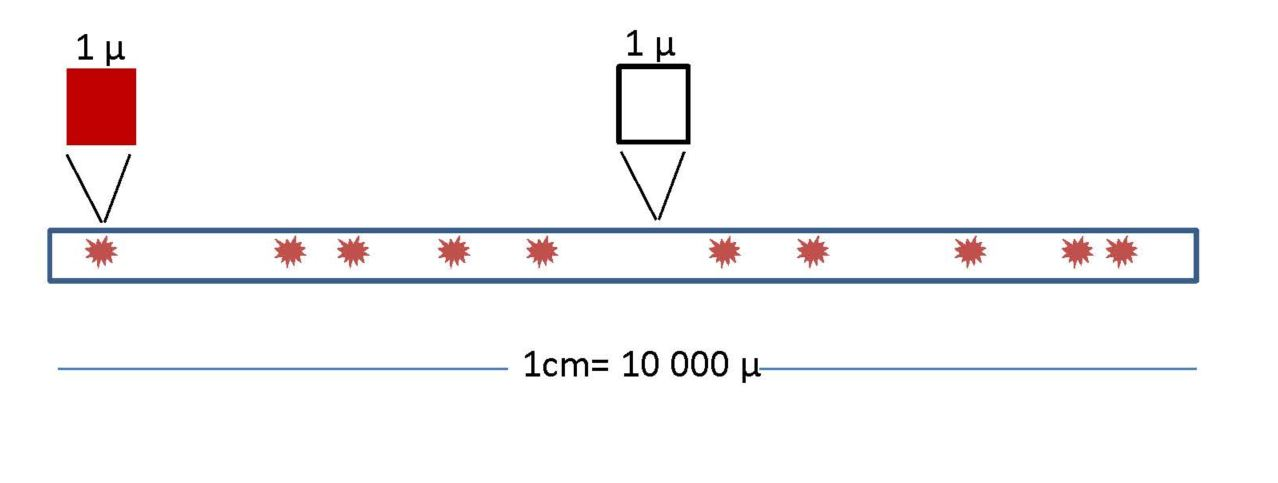
\includegraphics{./figures/Pois.JPG}

\textbf{De la función binomial a la función de probabilidad de Poisson}

La probabilidad de observar \(X\) impurezas en \(n=10,000\mu\) (1cm) sigue aproximadamente una distribución binomial

\[f(x) \sim \binom nxp^x(1-p)^{nx}\]

donde \(p\) es la probabilidad de encontrar una impureza en un micrómetro.

Dado que el valor esperado de una variable Binomial es \(E(X)=np\). Este es el número promedio de impurezas por 1 cm o \(\lambda=np\). Por lo tanto, sustituimos \(p=\lambda/n\)

\[f(x) \sim \binom nx \big(\frac{\lambda}{n}\big)^x(1-\frac{\lambda}{n})^{nx}\]

Dado que \textbf{podría} haber todavía dos impurezas en un micrómetro, necesitamos aumentar la partición del alambre y \(n \rightarrow \infty\).

Luego en el límite:

\[f(x)= \frac{e^{-\lambda}\lambda^x}{x!}\]

Donde \(\lambda\) es constante porque es la densidad de impurezas por centímetro, una \textbf{propiedad física} del sistema. \(\lambda\) es por lo tanto el \textbf{parámetro} del modelo de probabilidad.

\textbf{Detalles de la derivación:}

Para \(f(x) \sim \binom nx \big(\frac{\lambda}{n}\big)^x(1-\frac{\lambda}{n})^{nx}\)

en el límite (\(n \rightarrow \infty\))

\begin{enumerate}
\def\labelenumi{\arabic{enumi})}
\tightlist
\item
  \(\frac{1}{n^x}\binom n x =\frac{1}{n^x}\frac{n!}{x! (n-x)!}=\frac{(n-x)!(n-x+1)...(n-1)n}{n^x x! (n-x)!}=\frac{n(n-1)..(n-x+1)}{n^x x!} \rightarrow \frac{1}{x!}\)
\item
  \((1-\frac{\lambda}{n})^{n} \rightarrow e^{-\lambda}\) (definition of exponential)
\item
  \((1-\frac{\lambda}{n})^{-x} \rightarrow 1\)
\end{enumerate}

Poniendo todo junto entonces:

\(f(x)= \frac{e^{-\lambda}\lambda^x}{x!}\)

\textbf{Definición}

Dado

\begin{enumerate}
\def\labelenumi{\arabic{enumi})}
\tightlist
\item
  un intervalo en los números reales
\item
  hay eventos que ocurren al azar en el intervalo
\item
  se conoce el número promedio de eventos en el intervalo (\(\lambda\))
\item
  si se puede encontrar una pequeña partición regular del intervalo tal que en cada partición la podamos considerar como un ensayo de Bernoulli.
\end{enumerate}

Entonces, la variable aleatoria \(X\) que cuenta eventos a lo largo del intervalo es una variable \textbf{Poisson} con función de masa de probabilidad
\[f(x)= \frac{e^{-\lambda}\lambda^x}{x!}, \lambda>0\]

\textbf{Propiedades:}
Cuando \(X \rightarrow Poiss(\lambda)\) tiene

\begin{enumerate}
\def\labelenumi{\arabic{enumi})}
\tightlist
\item
  media \[E(X)= \lambda\]
\item
  y varianza \[V(X)= \lambda\]
\end{enumerate}

\textbf{Ejemplos}

\begin{enumerate}
\def\labelenumi{\arabic{enumi})}
\tightlist
\item
  ¿Cuál es la probabilidad de recibir 4 correos electrónicos en una hora, cuando el promedio de correos electrónicos en una hora es de \(1\)?
\end{enumerate}

Tenemos que la varible es de Poisson: \(X \rightarrow Poiss(\lambda)\) con \(\lambda=1\) y su función de masa de probabilidad es:

\[f(x)= \frac{e^{-1}1^x}{x!}\]
Por lo tanto la probabilidad de que la variable tome valor 4 es \(P(X=4)\):

\(f(4; \lambda=1)= \frac{e^{-1}1^4}{4!}=0.01532831\)

in R dpois(4,1)

\begin{enumerate}
\def\labelenumi{\arabic{enumi})}
\setcounter{enumi}{1}
\tightlist
\item
  ¿Cuál es la probabilidad de recibir 4 correos electrónicos en \textbf{tres horas}, cuando el promedio de correos electrónicos en una hora es de \(1\)?
\end{enumerate}

La unidad sobre la cual hacemos los conteos ha cambiado de 1 hora a 2 horas, por lo tanto tenemos que \textbf{re-escalar} \(\lambda\). Si antes el promedio de correos era \(\lambda=1\) en una hora, el promedio de correos en tres horas es ahora 3: \(\lambda_{3h}=3\lambda_{1h}=3*1=3\)

Tenemos que la varible es de Poisson: \(X \rightarrow Poiss(\lambda_{3h})\) con \(\lambda_{3h}=3\) y su función de masa de probabilidad es:

\[f(x)= \frac{e^{-3}3^x}{x!}\]
Por lo tanto la probabilidad de que la variable tome valor 4 es \(P(X=4)\):

\(f(4; \lambda=3)= \frac{e^{-3}3^4}{4!}=0.1680314\)

in R dpois(4,3)

\begin{enumerate}
\def\labelenumi{\arabic{enumi})}
\setcounter{enumi}{2}
\tightlist
\item
  ¿Cuál es la probabilidad de contar \textbf{al menos} \(10\) automóviles que llegan a un peaje en un minuto, cuando el promedio de automóviles que llegan a un peaje en un minuto es de \(5\);
\end{enumerate}

Tenemos que la varible es de Poisson: \(X \rightarrow Poiss(\lambda)\) con \(\lambda=5\) y su función de masa de probabilidad es:

\[f(x)= \frac{e^{-5}5^x}{x!}\]

\(P(X\geq 10)=1-P(X < 10)=1-P(X \leq 9)=1-F(9; \lambda=5)=1-\sum_{x=0, ...10}f(x; \lambda=5)=0.03182806\)

en R 1-ppois(9,5)

Veamos algunas funciones de masa de probabilidad en la familia de modelos paramétricos de Poisson:

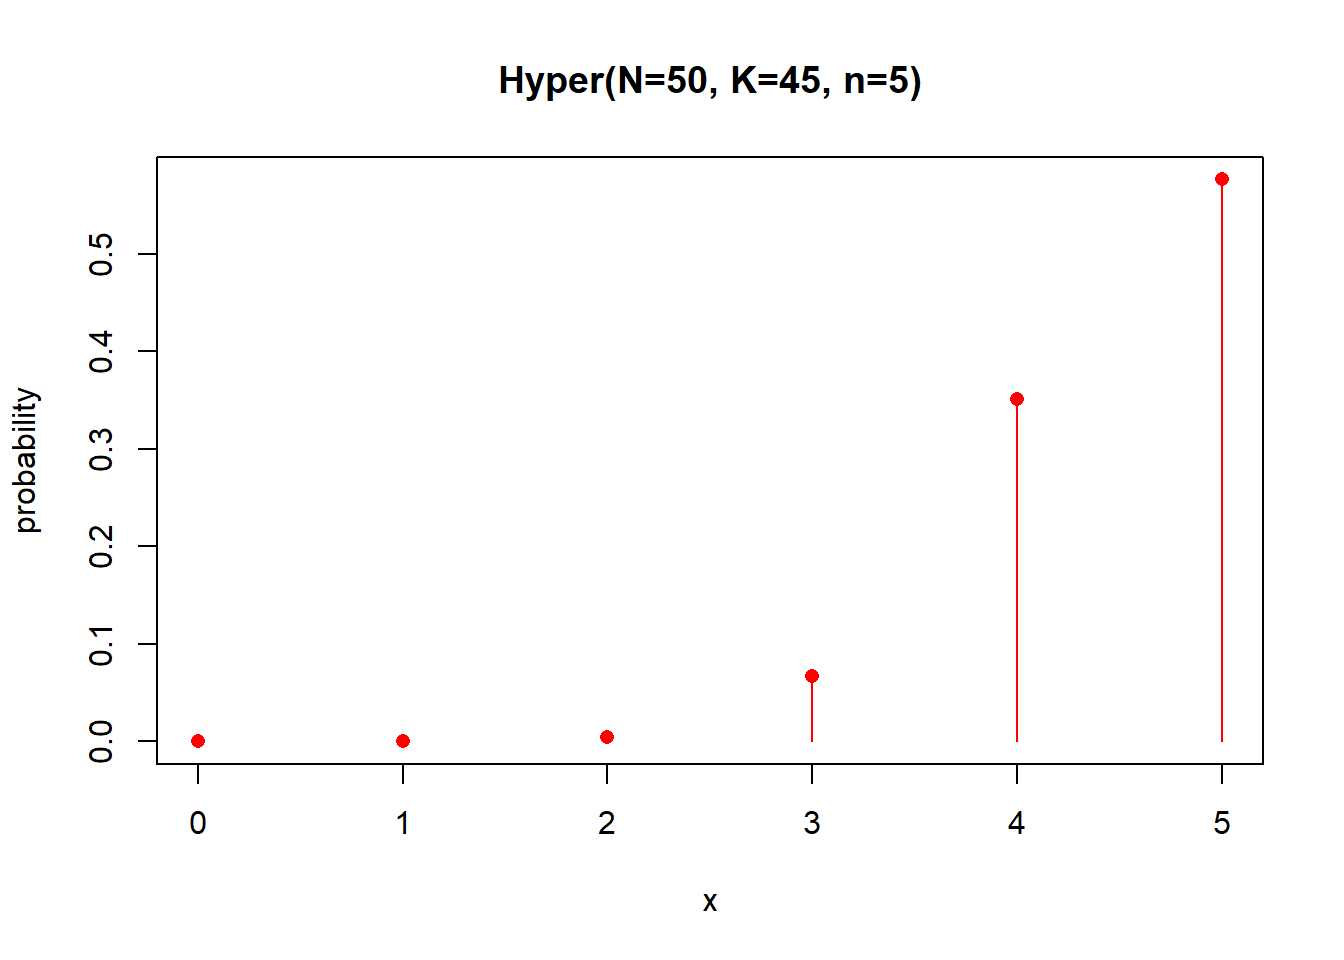
\includegraphics{_main_files/figure-latex/unnamed-chunk-61-1.pdf}

\hypertarget{modelos-de-probabilidad-para-variables-continuas}{%
\section{Modelos de probabilidad para variables continuas}\label{modelos-de-probabilidad-para-variables-continuas}}

Los modelos de probabilidad para variables continuas son \textbf{funciones de densidad} de probabilidad \(f(x)\) que \textbf{creemos} describen experimentos aleatorios reales.

La función de densidad de probabilidad \(f(x)\)

\begin{enumerate}
\def\labelenumi{\arabic{enumi})}
\tightlist
\item
  es positiva
\end{enumerate}

\[f(x) \geq 0\]

\begin{enumerate}
\def\labelenumi{\arabic{enumi})}
\setcounter{enumi}{1}
\tightlist
\item
  nos permite calcular probabilidades usando el área bajo la curva:
\end{enumerate}

\[P(a\leq X \leq b)=\int_{a}^{b} f(x) dx\]

\begin{enumerate}
\def\labelenumi{\arabic{enumi})}
\setcounter{enumi}{2}
\tightlist
\item
  es tal que la probabilidad de que obtengamos cualquier resultado es \(1\):
\end{enumerate}

\[\int_{-\infty}^{\infty} f(x) dx = 1\]

\hypertarget{experimento-exponencial}{%
\section{Experimento exponencial}\label{experimento-exponencial}}

Volvamos a un \textbf{proceso de Poisson} definido por la probabilidad

\[f(k)=\frac{e^{-\lambda}\lambda^k}{k!}, \lambda>0\]

para el número de eventos (\(k\)) en un intervalo.

Consideremos ahora que estamos interesados en la duración/tiempo que debemos esperar hasta que ocurra el \textbf{primer} conteo.

Podemos preguntarnos por la probabilidad de que el primer evento ocurra después de la duración/tiempo \(X\).

Por lo tanto, dado que \(X\) es una variable aleatoria \textbf{continua}, buscamos su función de densidad de probabilidad \(f(x)\).

\hypertarget{densidad-de-probabilidad-exponencial}{%
\section{Densidad de probabilidad exponencial}\label{densidad-de-probabilidad-exponencial}}

La probabilidad de \(0\) eventos \textbf{si} un intervalo tiene unidad \(x\) (rescalando como en el ejemplo 2) es

\[f(0|x)=\frac{e^{-x\lambda}(x\lambda)^0}{0!}\]

o

\[f(0|x)=e^{-x\lambda}\]

Podemos tratar esto como la probabilidad condicional de \(0\) eventos dada una distancia \(x\): \(f(K=0|X=x)\) y aplicar el teorema de Bayes para invertirlo:

\[f(x|0)=C f(0|x)=C e^{-x\lambda}\]

Esta es la \textbf{probabilidad de observar una distancia} \(x\) para \(0\) eventos. Esta es la distancia hasta el primer evento.

\textbf{Definición}

En un proceso de Poisson con parámetro \(\lambda\) la probabilidad de esperar una distancia/tiempo \(X\) entre dos conteos viene dada por la \textbf{densidad de probabilidad}

\[f(x)= C e^{-x\lambda}\]

\begin{itemize}
\item
  \(C\) es una constante que asegura: \(\int_{-\infty}^{\infty} f(x) dx =1\)
\item
  por integración \(C=\lambda\)
\end{itemize}

Por lo tanto:

\[f(x)=\lambda e^{-\lambda x}, x\geq 0\]

\(\lambda\) es el parámetro del modelo, también conocido como \textbf{tasa de decaimiento}.

\textbf{Propiedades:}

Cuando \(X \rightarrow Exp(\lambda)\) entonces

\begin{enumerate}
\def\labelenumi{\arabic{enumi})}
\tightlist
\item
  tiene media
\end{enumerate}

\[E(X)=\frac{1}{\lambda}\]

\begin{enumerate}
\def\labelenumi{\arabic{enumi})}
\setcounter{enumi}{1}
\tightlist
\item
  y varianza
  \[V(Y)=\frac{1}{\lambda^2}\]
\end{enumerate}

Veamos un par de densidades de probabilidad en la familia exponencial

\includegraphics{_main_files/figure-latex/unnamed-chunk-62-1.pdf}

\hypertarget{distribuciuxf3n-exponencial}{%
\section{Distribución exponencial}\label{distribuciuxf3n-exponencial}}

Consideremos las siguientes preguntas:

\begin{enumerate}
\def\labelenumi{\arabic{enumi})}
\tightlist
\item
  En un proceso de Poisson ¿Cuál es la probabilidad de observar un intervalo \textbf{menor} que \(a\) hasta el primer evento?
\end{enumerate}

Recuerda que esta probabilidad \(F(a)=P(X \leq a)\) es la densidad de probabilidad

\[F(a)=\lambda\int_\infty^ae^{-x\lambda}dx=1-e^{-a\lambda}\]
2) En un proceso de Poisson ¿Cuál es la probabilidad de observar un intervalo \textbf{mayor} que \(a\) hasta el primer evento?

\[P(X > a)=1- P(X \leq a)= 1- F(a) = e^{-a\lambda}\]

Veamos un par de distribuciones exponenciales de la familia exponencial

\includegraphics{_main_files/figure-latex/unnamed-chunk-63-1.pdf}

La mediana \(x_m\) es tal que \(F(x_m)=0.5\). Eso es \(x_m=\frac{\log(2)}{\lambda}\)

\textbf{Ejemplos}

\begin{enumerate}
\def\labelenumi{\arabic{enumi})}
\tightlist
\item
  ¿Cuál es la probabilidad de que tengamos que esperar un bus por más de \(1\) hora cuando en promedio hay dos buses por hora?
\end{enumerate}

\[P(X > 1)=1-P(X \le 1) = 1-F(1,\lambda=2)=0.1353353\]

En R 1-pexp(1,2)

\begin{enumerate}
\def\labelenumi{\arabic{enumi})}
\setcounter{enumi}{1}
\tightlist
\item
  ¿Cuál es la probabilidad de tener que esperar menos de \(2\) segundos para detectar una partícula cuando la tasa de desintegración radiactiva es de \(2\) partículas por segundo; \(F(2,\lambda=2)\)
\end{enumerate}

\[P(X\le 2)=F(2,\lambda=2)=0.9816844\]

En R pexp(2,2)

\hypertarget{preguntas-5}{%
\section{Preguntas}\label{preguntas-5}}

\textbf{1)} Durante la Segunda Guerra Mundial, en un día de bombardeo sobre Londres, el valor eperado de que cayera una bomba en \(1.5km^2\) era de \(0.92\). La probabilidad de que en Hyde Park, de área aproximadamente \(1.5km^2\), cayeran como mucho dos bombas era de

\textbf{\(\qquad\)a:}1-ppois(x=2, lambda=0.92);
\textbf{\(\qquad\)b:}ppois(x=2, lambda=0.92); \textbf{\(\qquad\)c:}1-dpois(x=2, lambda=0.92); \textbf{\(\qquad\)d:}dpois(x=2, lambda=0.92)

\textbf{2)} La probabilidad de que un pasajero tenga que esperar menos de 20 minutos hasta que llegue el próximo taxi a su parada está mejor descrita por

\textbf{\(\qquad\)a:} Un modelo de Poisson sobre el número de taxis que pasan cada 20 minutos;
\textbf{\(\qquad\)b:} Una distribución exponencial con \(\lambda=1/20\) ;
\textbf{\(\qquad\)c:} Un modelo binomial que cuenta el número de taxis cada 20 minutos
\textbf{\(\qquad\)d:} Una distribución uniforme entre 0 y 20 minutos;

\textbf{3)} A partir de la distribución de probabilidad exponencial de la siguiente figura, ¿cuál es el valor más posible de la mediana?

\textbf{\(\qquad\)a:} \(2\); \textbf{\(\qquad\)b:} \(3\); \textbf{\(\qquad\)c:} \(4\); \textbf{\(\qquad\)d:} \(5\)

\includegraphics{./figures/exp.png}

\hypertarget{ejercicios-6}{%
\section{Ejercicios}\label{ejercicios-6}}

\hypertarget{ejercicio-1-5}{%
\subsubsection{Ejercicio 1}\label{ejercicio-1-5}}

El promedio de llamadas telefónicas por hora que ingresan a la centralita de una empresa es de \(150\). Encuentra la probabilidad de que durante un minuto en particular haya

\begin{itemize}
\tightlist
\item
  0 llamadas telefónicas (R:0.082)
\item
  1 llamada telefónica (R:0.205)
\item
  4 o menos llamadas (R:0.891)
\item
  más de 6 llamadas telefónicas (R:0.0141)
\end{itemize}

\hypertarget{ejercicio-2-5}{%
\subsubsection{Ejercicio 2}\label{ejercicio-2-5}}

La cantidad promedio de partículas radiactivas que golpean un contador Geiger en una planta de energía nuclear bajo control es de \(2.3\) por minuto.

\begin{itemize}
\item
  ¿Cuál es la probabilidad de contar exactamente \(2\) partículas en un minuto? (R:0.265)
\item
  ¿Cuál es la probabilidad de detectar exactamente \(10\) partículas en \(5\) minutos? (R:0.112)
\item
  ¿Cuál es la probabilidad de al menos un conteo en dos minutos? (R:0.9899)
\item
  ¿Cuál es la probabilidad de tener que esperar menos de \(1\) segundo para detectar una partícula radiactiva, después de encender el detector? (R:0.037)
\item
  Sospechamos que una planta nuclear tiene una fuga radiactiva si esperamos menos de \(1\) segundo para detectar una partícula radiactiva, después de encender el detector. ¿Cuál es la probabilidad de que cuando visitemos \(5\) plantas que están bajo control, sospechemos que al menos una tiene una fuga? (R:0.1744).
\end{itemize}

\hypertarget{distribuciuxf3n-normal}{%
\chapter{Distribución normal}\label{distribuciuxf3n-normal}}

\hypertarget{objetivo-5}{%
\section{Objetivo}\label{objetivo-5}}

En este capítulo introduciremos la distribución de probabilidad normal.

Hablaremos de su origen y de sus principales propiedades.

\hypertarget{historia}{%
\section{Historia}\label{historia}}

En 1801, Gauss analizó los datos obtenidos sobre la posición de Ceres, un gran asteroide entre Marte y Júpiter.

En ese momento, la gente sospechaba que era un nuevo planeta, ya que se movía día a día contra las estrellas fijas. En enero, se podía ver en el horizonte justo antes del amanecer. Sin embargo, a medida que pasaban los días, Ceres salía cada vez más tarde hasta que ya no se pudo ver más debido a la salida del Sol.

Gauss entendió que las medidas para la posición de Ceres tenían errores.

Por lo tanto, estaba interesado en descubrir cómo se \textbf{distribuían} las observaciones para poder encontrar la órbita más \textbf{probable}. Con la órbita, podía derivar la masa del objeto y luego decidir si era un planeta o sólo un gran asteroide.

Los datos estaban disponibles sólo para el mes de enero. Después de lo cual Ceres desaparecería. Quería \textbf{predecir} hacia dónde deberían apuntar los astrónomos sus telescopios para encontrarlo seis meses después al anochecer, una vez que hubiera pasado por detrás del Sol.

Gauss tuvo que dar cuenta de los errores en la posición de ceres en un día determinado debido a la medición

\includegraphics{./figures/ceres.JPG}

Gauss supuso que

\begin{enumerate}
\def\labelenumi{\arabic{enumi})}
\item
  los errores pequeños eran más probables que los errores grandes
\item
  el error a una distancia \(-\epsilon\) del varlor en la posición de Ceres era igualmente probable que una distancia \(\epsilon\)
\item
  la pisición más \textbf{verosimil} (que nos creemos más) de Ceres en un momento dado en el cielo era el \textbf{promedio} de múltiples mediciones de altitud en esa latitud.
\end{enumerate}

Eso fue suficiente para mostrar que las desviaciones de las observaciones \(y\) \textbf{de la órbita} satisfacian la ecuación

\[\frac{df(y)}{dy}=-Cyf(y)\]
con \(C\) una costante positiva. La solución de esta ecuación diferencial es:

\[f(y)=\frac{\sqrt{C}}{\sqrt{2\pi}}e^{-\frac{Cy^2}{2}}\]

*The evolution of the normal distribution, Saul Stahl, Mathemetics Magazine, 2006.

\hypertarget{densidad-normal}{%
\section{Densidad normal}\label{densidad-normal}}

Densidad de probabilidad de Gauss da la distribución de los errores de medición desde la posición \textbf{real} pero \textbf{desconocida} de Ceres en el cielo. Hagamos un par de cambios en la función.

1- Escribamos la densidad de errores desde el horizonte usando la variable aleatoria \(X\), o sea \(y=x-\mu\). \(\mu\) es la posición \textbf{real} pero \textbf{desconocida} de Ceres desde el horizonte. Después de un cambio de variable encontramos la función de densidad de probabilidad:

\[f(x)=\frac{\sqrt{C}}{\sqrt{2\pi}}e^{-C(x-\mu)^2}\]

\begin{enumerate}
\def\labelenumi{\arabic{enumi})}
\setcounter{enumi}{1}
\tightlist
\item
  Cambiemos de nombre la variable \(C\) por \(\frac{1}{\sigma^2}\)
\end{enumerate}

Entonces, llegamos a la siguente definición.

\hypertarget{definiciuxf3n}{%
\section{Definición}\label{definiciuxf3n}}

Una variable aleatoria \(X\) definida en los números reales tiene una densidad \textbf{Normal} si toma la forma

\[f(x; \mu, \sigma^2)=\frac{1}{\sqrt{2\pi}\sigma}e^{-\frac{(x-\mu)^2}{2\sigma^2}}, x \in {\mathbb R}\]

La variable tiene

\begin{enumerate}
\def\labelenumi{\arabic{enumi})}
\tightlist
\item
  media
\end{enumerate}

\[E(X) = \mu\]

que para Gauss representaba la posición real de Ceres.

\begin{enumerate}
\def\labelenumi{\arabic{enumi})}
\setcounter{enumi}{1}
\tightlist
\item
  y varianza
  \[V (X) = \sigma^2\]
\end{enumerate}

que representaba la dispersión del error en las observaciones, que depende de la calidad del telescopio.

\(\mu\) y \(\sigma\) son los \textbf{dos parámetros} que describen completamente la función de densidad normal y su \textbf{interpretación} depende del experimento aleatorio.

Cuando \(X\) sigue una densidad Normal, es decir, se distribuye normalmente, escribimos

\[X\rightarrow N(\mu,\sigma^2)\]

Veamos algunas densidades de probabilidad en el modelo paramétrico normal

\includegraphics{_main_files/figure-latex/unnamed-chunk-64-1.pdf}

\hypertarget{distribuciuxf3n-de-probabilidad-2}{%
\section{Distribución de probabilidad}\label{distribuciuxf3n-de-probabilidad-2}}

La distribución de probabilidad de la densidad Normal:

\[F(a)=P(Z \leq a)\]

es la función de \textbf{error} definida por el área bajo la curva de \(-\infty\) a \(a\)

\[F(a)=\int_{-\infty}^{a}\frac{1}{\sqrt{2\pi}\sigma}e^{-\frac{(x-\mu) ^2}{2\sigma^2}} dx\]
La función se encuentra en la mayoría de los programas de computadora y no tiene una forma cerrada de funciones conocidas.

\textbf{Ejemplo (altura de mujeres)}

\begin{enumerate}
\def\labelenumi{\arabic{enumi})}
\tightlist
\item
  ¿Cuál es la probabilidad de que una mujer de la población tenga una altura máxima de \(150 cm\) si las mujeres tienen una altura media de \(165 cm\) con una desviación estándar de \(8 cm\)?
\end{enumerate}

\(P(X\le 150)=F(150, \mu=165, \sigma=8)=0.03039636\)

en R pnorm(150, 165, 8)

\begin{enumerate}
\def\labelenumi{\arabic{enumi})}
\setcounter{enumi}{1}
\tightlist
\item
  ¿Cuál es la probabilidad de que la altura de una mujer en la población esté entre \(165cm\) y \(170cm\)?
\end{enumerate}

\(P(165 \le X \le 170)=F(170, \mu=165, \sigma=8)-F(165, \mu=165, \sigma=8)=0.2340145\)

en R pnorm(170, 165, 8)-pnorm(165, 165, 8)

Veamos la función de distribución de probabilidad

\includegraphics{_main_files/figure-latex/unnamed-chunk-65-1.pdf}

\begin{enumerate}
\def\labelenumi{\arabic{enumi})}
\setcounter{enumi}{2}
\tightlist
\item
  ¿Cuál es el primer cuartíl para altura de las mujeres?
\end{enumerate}

El primer cuartíl se define como:

\(F(x_{0.25}, \mu=165, \sigma=8)=0.25\)

o

\(x_{0.25}=F^{-1}(0.25, \mu=165, \sigma=8)=159.6041\)

en R qnorm(0.25, 165, 8)

\textbf{Propiedades de la distribución Normal}

\begin{enumerate}
\def\labelenumi{\arabic{enumi})}
\item
  la media \(\mu\) es también la mediana ya que divide las medidas en dos
\item
  Los valores de \(x\) que caen más allá de 2\(\sigma\) se consideran \textbf{raros} \(5\%\)
\item
  Los valores de \(x\) que caen más allá de 3\(\sigma\) se consideran \textbf{extremadamente raros} \(0.2\%\)
\end{enumerate}

\includegraphics{./figures/probs.png}

\textbf{Ejemplo (altura de mujeres)}

Podemos definir los límites de \textbf{observaciones comunes} para la distribución de la altura de las mujeres en la población.

\begin{enumerate}
\def\labelenumi{\arabic{enumi})}
\tightlist
\item
  a una distancia de una desviación estándar de la media, encontramos \(68\%\) de la población
\end{enumerate}

\[P(165-8 \leq X \leq 165+8)=P(157 \leq X \leq 173)=F(173)-F(157)=0.68\]

\begin{enumerate}
\def\labelenumi{\arabic{enumi})}
\setcounter{enumi}{1}
\tightlist
\item
  a una distancia de dos desviaciones estándar de la media, encontramos \(95\%\) de la población
\end{enumerate}

\[P(165-2 \times 8 \leq X \leq 165+2\times 8)=F(181)-F(149)=0.95\]

\begin{enumerate}
\def\labelenumi{\arabic{enumi})}
\setcounter{enumi}{2}
\tightlist
\item
  a una distancia de tres desviaciones estándar de la media, encontramos \(99.7\%\) de la población
\end{enumerate}

\[P(165-3 \times 8 \leq X \leq 165+3\times 8)=F(189)-F(141)=0.997\]

\includegraphics{_main_files/figure-latex/unnamed-chunk-66-1.pdf}

\hypertarget{densidad-normal-estuxe1ndar}{%
\section{Densidad normal estándar}\label{densidad-normal-estuxe1ndar}}

La densidad normal estándar es la densidad particular de la familia normal

\[f(x; \mu, \sigma^2)=\frac{1}{\sqrt{2\pi}\sigma}e^{-\frac{(x-\mu)^2}{2\sigma^2}}, x \in {\mathbb R}\]

Por lo tanto, es la densidad con

\begin{enumerate}
\def\labelenumi{\arabic{enumi})}
\tightlist
\item
  media
\end{enumerate}

\[E(X)= \mu = 0\]

\begin{enumerate}
\def\labelenumi{\arabic{enumi})}
\setcounter{enumi}{1}
\tightlist
\item
  y varianza
\end{enumerate}

\[V (X)= \sigma^2 =1\]

Cuando una variable aleatoria sigue una densidad de probabilidad normal, decimos que se distribuye normalmente y escribimos

\[X \rightarrow N(0,1)\]

\hypertarget{distribuciuxf3n-estuxe1ndar}{%
\section{Distribución estándar}\label{distribuciuxf3n-estuxe1ndar}}

La distribución estándar es:

\[\phi(a)=F_{N(0,1)}(a)=P(Z \leq a)\]

es la función \textbf{error} definida por

\[\phi(a)=\int_{-\infty}^{a} \frac{1}{\sqrt{2\pi}}e^{-\frac{z^2}{2}} dz\]

Debido a que la distribución estándar es especial y aparecerá con frecuencia, usamos la letra \(\phi\) para ello.

\includegraphics{./figures/st.png}

Puedes encontrarla en la mayoría de los programas de computadora. En R es pnorm(x) con los parámetros predeterminados, 0 y 1.

Normalmente definimos los límites de las \textbf{observaciones más comunes} para la variable estándar

\includegraphics{./figures/phi.JPG}

\begin{enumerate}
\def\labelenumi{\arabic{enumi})}
\tightlist
\item
  El rango intercuartílico \[P(-0.67 \leq X \leq 0.67)=0.50\]
\end{enumerate}

en R: c(qnorm(0.25), qnorm(0.75))

\begin{enumerate}
\def\labelenumi{\arabic{enumi})}
\setcounter{enumi}{1}
\tightlist
\item
  El rango del \(95\%\) \[P(-1.96 \leq X \leq 1.96)=0.95\]
\end{enumerate}

en R: c(qnorm(0.025), qnorm(0.975))

\begin{enumerate}
\def\labelenumi{\arabic{enumi})}
\setcounter{enumi}{2}
\tightlist
\item
  El rango del \(99\%\) \[P(-2.58 \leq X \leq 2.58)=0.99\]
\end{enumerate}

en R: c(qnorm(0.005), qnorm(0.995))

\includegraphics{_main_files/figure-latex/unnamed-chunk-67-1.pdf}

\hypertarget{estandarizaciuxf3n}{%
\section{Estandarización}\label{estandarizaciuxf3n}}

Todas las variables normales se pueden \textbf{estandarizar}. Esto significa que si \(X \rightarrow N(\mu, \sigma^2)\), entonces podemos transformar la variable a
una \textbf{variable estandarizada}

\[Z=\frac{X-\mu}{\sigma}\]

que tendrá densidad:

\[f(z)=\frac{1}{ \sqrt{2\pi}}e^{-\frac{z^2}{2}}\]
Por lo tanto, para cualquier \(X \rightarrow N(\mu, \sigma^2)\)

\[Z=\frac{X-\mu}{\sigma} \rightarrow N(0, 1) \]

\includegraphics{./figures/stand.png}

Puedes demostrar esto reemplazando \(x=\sigma z+\mu\) y \(dx=\sigma dz\) en la expresión de probabilidad que tenemos

\(P(x\leq X \leq x +dx)=P(z\leq Z \leq z +dz)\)
\[=\frac{1}{\sqrt{2\pi}\sigma}e^{-\frac{(x-\mu)^2}{2\sigma^2}}dx\] \[=\frac{1}{ \sqrt{2\pi}}e^{-\frac{z^2}{2}} dz\]

La probabilidad de \textbf{cualquier variable normal} \(X\rightarrow N(\mu, \sigma^2)\) se puede calcular usando la distribución estándar

\(F(a)=P(X<a)=P(\frac{X-\mu}{\sigma}<\frac{a-\mu}{\sigma})\)
\[=P(Z < \frac{a-\mu}{\sigma})= \phi \big(\frac{a-\mu}{\sigma}\big)\]

Para calcular \(P(a\leq X \leq b)\), usamos la propiedad de las distribuciones de probabilidad

\(F(b)-F(a)=P(X\leq b)-P(X\leq a)\)

\[=\phi \big(\frac{b-\mu}{\sigma}\big)-\phi \big(\frac{a-\mu}{\sigma}\big)\]

\hypertarget{resumen-de-modelos-de-probabilidad}{%
\section{Resumen de modelos de probabilidad}\label{resumen-de-modelos-de-probabilidad}}

\begin{longtable}[]{@{}
  >{\centering\arraybackslash}p{(\columnwidth - 10\tabcolsep) * \real{0.1667}}
  >{\centering\arraybackslash}p{(\columnwidth - 10\tabcolsep) * \real{0.1905}}
  >{\centering\arraybackslash}p{(\columnwidth - 10\tabcolsep) * \real{0.1905}}
  >{\centering\arraybackslash}p{(\columnwidth - 10\tabcolsep) * \real{0.1667}}
  >{\centering\arraybackslash}p{(\columnwidth - 10\tabcolsep) * \real{0.1429}}
  >{\centering\arraybackslash}p{(\columnwidth - 10\tabcolsep) * \real{0.1429}}@{}}
\toprule\noalign{}
\begin{minipage}[b]{\linewidth}\centering
Modelo
\end{minipage} & \begin{minipage}[b]{\linewidth}\centering
X
\end{minipage} & \begin{minipage}[b]{\linewidth}\centering
rango de x
\end{minipage} & \begin{minipage}[b]{\linewidth}\centering
f(x)
\end{minipage} & \begin{minipage}[b]{\linewidth}\centering
E(X)
\end{minipage} & \begin{minipage}[b]{\linewidth}\centering
V(X)
\end{minipage} \\
\midrule\noalign{}
\endhead
\bottomrule\noalign{}
\endlastfoot
Uniforme & número entero o real & \([a,b]\) & \(\frac{1}{n}\) & \(\frac{b+a}{2}\) & \(\frac{(b-a+1)^2-1}{12}\) \\
Bernoulli & evento A (1) & 0,1 & \((1-p)^{1-x}p^x\) & \(p\) & \(p(1-p)\) \\
Binomial & \# de eventos A en \(n\) repeticiones de ensayos de Bernoulli & 0,1,\ldots{} & \(\binom nx (1-p)^{nx}p^x\) & \(np\) & \(np(1-p)\) \\
Binomial negativo para eventos & \# de eventos B (0) en repeticiones de Bernoulli antes de \(r\) eventos A (1) & 0,1,.. & \(\binom {x+r-1} x (1-p)^xp^r\) & \(\frac{r(1-p)}{p}\) & \(\frac{r(1-p)}{p^2}\) \\
Hipergeométrico & \# de eventos A en una muestra \(n\) de la población \(N\) con \(K\) numero de As & \(\max(0, n+KN)\), \ldots{} \(\min(K, n)\) & \(\frac{1}{\binom N n}\binom K x \binom {N-K} {n-x}\) & \(n*\frac{N}{K}\) & \(n \frac{N}{K} (1-\frac{N}{K})\frac{Nn}{N-1}\) \\
Poisson & \# de eventos A en un intervalo & 0,1, .. & \(\frac{e^{-\lambda}\lambda^x}{x!}\) & \(\lambda\) & \(\lambda\) \\
Exponencial & Intervalo entre dos eventos A & \([0,\infty)\) & \(\lambda e^{-\lambda x}\) & \(\frac{1}{\lambda}\) & \(\frac{1}{\lambda^2}\) \\
Normal & medida con errores simétricos cuyo valor más probable es la media & \((-\infty, \infty)\) & \(\frac{1}{\sqrt{2\pi}\sigma}e^{-\frac{(x-\mu)^2}{2\sigma^2 }}\) & \(\mu\) & \(\sigma^2\) \\
\end{longtable}

\hypertarget{funciones-r-de-modelos-de-probabilidad}{%
\section{Funciones R de modelos de probabilidad}\label{funciones-r-de-modelos-de-probabilidad}}

\begin{longtable}[]{@{}
  >{\raggedright\arraybackslash}p{(\columnwidth - 4\tabcolsep) * \real{0.3333}}
  >{\centering\arraybackslash}p{(\columnwidth - 4\tabcolsep) * \real{0.3333}}
  >{\centering\arraybackslash}p{(\columnwidth - 4\tabcolsep) * \real{0.3333}}@{}}
\toprule\noalign{}
\begin{minipage}[b]{\linewidth}\raggedright
modelo
\end{minipage} & \begin{minipage}[b]{\linewidth}\centering
R f(x)
\end{minipage} & \begin{minipage}[b]{\linewidth}\centering
R F(x)
\end{minipage} \\
\midrule\noalign{}
\endhead
\bottomrule\noalign{}
\endlastfoot
Uniforme (continuo) & dunif(x, a, b) & punif(x, a, b) \\
Binomial & dbinom(x,n,p) & pbimon(x,n,p) \\
Binomial negativo para eventos & dnbinom(x,r,p) & pnbinom(x,r,p) \\
Hipergeométrico & dhyper(x, K, N-K, n) & phyper(x, K, N-K, n) \\
Poisson & dpois(x, lambda) & ppois(x, lambda) \\
Exponencial & dexp(x, lambda) & pexp(x, lambda) \\
normales & dnorm(x, mu, sigma) & pnomr(x, mu, sigma) \\
\end{longtable}

\hypertarget{preguntas-6}{%
\section{Preguntas}\label{preguntas-6}}

\textbf{1)} Para una variable normal estándar

\textbf{\(\qquad\)a:} \(50\%\) de sus observaciones están entre \((-0.67,0.67)\);
\textbf{\(\qquad\)b:} \(2\%\) de sus observaciones son inferiores a \(-2.58\);
\textbf{\(\qquad\)c:} \(5\%\) de sus observaciones son superiores a \(1.96\);
\textbf{\(\qquad\)d:} \(25\%\) de sus observaciones están entre \((-1.96,-0.67)\)

\textbf{2)} si sabemos que \(\phi(-0.8416212)=0.2\) entonces que es \(\phi(0.8416212)\)

\textbf{\(\qquad\)a:} \(0.1\);
\textbf{\(\qquad\)b:} \(0.2\);
\textbf{\(\qquad\)c:} \(0.8\);
\textbf{\(\qquad\)d:} \(0.9\)

\textbf{3)} el tercer cuartil de una variable normal con media \(10\) y desviación estándar \(2\) es

\textbf{\(\qquad\)a:} qnorm(1/3, 10, 2)=9.138545;
\textbf{\(\qquad\)b:} qnorm(1-0.75, 10, 2)=8.65102 ;
\textbf{\(\qquad\)c:} qnorm(1-1/3, 10, 2)=10.86145 ;
\textbf{\(\qquad\)d:} qnorm(0.75, 10, 2)= 11.34898

\textbf{4)} la probabilidad de que una variable normal con media \(10\) y desviación estándar \(2\) esté en \((-\infty,10)\) es

\textbf{\(\qquad\)a:} 0.25;
\textbf{\(\qquad\)b:} 0.5;
\textbf{\(\qquad\)c:} 0.75;
\textbf{\(\qquad\)d:} 1:

\textbf{5)} No es cierto que para una variable normal estándar

\textbf{\(\qquad\)a:} su media y mediana son iguales; \textbf{\(\qquad\)b:} la distribución de probabilidad estándar se puede utilizar para calcular sus probabilidades; \textbf{\(\qquad\)c:} su rango intercuartílico es el doble de su desviación estándar; \textbf{\(\qquad\)d:} \(5\%\) de sus observaciones están a una distancia desde \(0\) mas grande que su desviación estándar

\hypertarget{ejercicios-7}{%
\section{Ejercicios}\label{ejercicios-7}}

\hypertarget{ejercicio-1-6}{%
\subsubsection{Ejercicio 1}\label{ejercicio-1-6}}

Encuentra el área bajo la curva normal estándar en los siguientes casos:

\begin{itemize}
\tightlist
\item
  Entre \(z=0.81\) y \(z=1.94\) (R:0.182)
\item
  A la derecha de \(z=-1.28\) (R:0.899)
\item
  A la derecha de \(z=2.05\) o a la izquierda de \(z=-1.44\) (R:0.0951)
\end{itemize}

\hypertarget{ejercicio-2-6}{%
\subsubsection{Ejercicio 2}\label{ejercicio-2-6}}

\begin{itemize}
\item
  ¿Cuál es la probabilidad de que la altura de un hombre sea al menos
  \(165\)cm si la media poblacional es \(175\)cm y la desviación estándar es \(10\)cm? (R:0.841)
\item
  ¿Cuál es la probabilidad de que la altura de un hombre esté entre
  \(165\)cm y \(185\)cm? (R:0.682)
\item
  ¿Cuál es la altura que define el \(5\%\) de los hombres más pequeños? (R:158.55)
\end{itemize}

  \bibliography{book.bib,packages.bib}

\end{document}
